\documentclass[12pt]{article}
\usepackage{ifpdf}
\ifpdf
\usepackage{cmap}
\pdfcompresslevel=9
\usepackage{graphicx}
\graphicspath{{image/}{image/Chapter_4/}{image/Chapter_6/}}
\usepackage{epstopdf}
\usepackage[pdftex, colorlinks=false, pdfstartview=FitH, hypertexnames=false, unicode, bookmarks=false]{hyperref} 
\else

\usepackage[hypertex, colorlinks=false, unicode]{hyperref}
\fi

\usepackage{amssymb, amsmath, amsxtra}
\usepackage{cite}

\usepackage{indentfirst}

%Цветной текст
\usepackage[usenames]{color}
\usepackage{colortbl}

\usepackage[cp1251]{inputenc}
\usepackage[T2A]{fontenc}
\usepackage{textcomp}
\usepackage[english,russian]{babel}



\usepackage{bm}
\usepackage{amsmath,amssymb,amsbsy} 
\usepackage{comment}
\def\mprp{\mbox{\tiny $\bot$}}
\def\mprl{\mbox{\tiny $\|$}}
\def\th{\mbox{th}}

\def\beq{\begin{eqnarray}}
\def\eeq{\end{eqnarray}}
\def\ee{\varepsilon}
\def\lm{\lambda}
\def\ff{\Lambda}
\def\tff{\widetilde \Lambda}
\def\1{1 \to 1 \, 2}
\def\2{1 \to 2 \, 2}

\def\beq{\begin{eqnarray}}
\def\eeq{\end{eqnarray}}
\def\ee{\varepsilon}
\def\lm{\lambda}

\newcommand{\bs}{\boldsymbol} 
\newcommand{\prp}[1]{#1_{\mbox{\tiny $\bot$}}}
\newcommand{\prl}[1]{#1_{\mbox{\tiny $\|$}}}



\newcommand{\ii}{\mathrm{i}}
\newcommand{\dd}{\mathrm{d}}
\newcommand{\eee}{\mathrm{e}} 
% Номера страниц сверху и по центру
%\def\headfont{\small}
%\pagestyle{headcenter}
%\chapterpagestyle{empty}

% Использовать полужирное начертание для векторов
\let\vec=\mathbf

\textheight 230mm  
\textwidth 170mm
\topmargin -5mm
\oddsidemargin 5mm

\pagestyle{plain}

\title{Резонансные процессы в активной среде}
\author{Д.А.~Румянцев$^{*}$, Д.М.~Шленев$^{**}$
А.А.~Ярков$^{***}$
\\
{\it Ярославский государственный университет им. П.Г. Демидова, Россия}}

\date{}

\begin{document}
\large
\maketitle
\def\abstractname{\empty}
\baselineskip=22pt

\begin{abstract}

\baselineskip=20pt

{\large В работе рассмотрены различные квантовые процессы с учетом резонанса на виртуальном фермионе.}
\end{abstract}

{\def\thefootnote{*}
\footnotetext{E-mail:  rda@uniyar.ac.ru}
\def\thefootnote{**}
\footnotetext{E-mail: allen\_caleb@rambler.com}
\def\thefootnote{***}
\footnotetext{E-mail: a12l@mail.ru}}

\newpage
\unitlength 1mm

%%%%%%%%%%%%%%%%%%%%%%%%%%%%%%%%%%%%%%%%%%%%%%%%%%%%%%%%%%%%%%%%%%%


\section{Введение}
Резонансные явления в нашей жизни встречаются повсеместно. Большинство этих явлений так или иначе связано с колебательными процессами. Так, резонанс в колебательном контуре даeт возможность получать или передавать информацию 
на определенной частоте с минимально затраченной энергией. При этом, в 
классическом подходе резонанс -- это резкое возрастание амплитуды колебаний при 
приближении частоты внешнего воздействия к собственной частоте системы. С 
другой стороны, в квантовом подходе в силу существования дискретных уровней 
энергии резонанс означает резкое увеличение вероятностей процессов, связанных с 
переходами между этими уровнями, таких как, например, поглощение фотона с 
энергией, равной разнице энергий между двумя состояниями электрона. Одним из 
условий, при которых учет квантовых эффектов при движении частиц становится 
необходимым, является присутствие сильных магнитных полей, чья индукция 
приближается к характерному значению, называемому критическим, $B_e = m^2 / e 
\simeq 4.41 \times 10^{13}$ Гс \footnote{В работе используется естественная 
система единиц: $\hbar = c = k = 1$, $m$ -- масса электрона, $e > 0$ --  
элементарный заряд.}. В природе такими экстремально большими магнитными полями, 
согласно современным моделям~\cite{Duncan:1995,Thompson:1996,Thompson:2002}, 
обладают разновидности нейтронных звезд, называемые радиопульсарами (с 
магнитными полями порядка $10^{12}$ Гс) и магнитарами (до $10^{15}$ 
Гс)~\cite{McGill:Cite}.

Кроме сильных магнитных полей в магнитосфере как радиопульсаров, так и магнитаров присутствует относительно горячая и плотная электрон-позитронная плазма~\cite{Duncan:1995}. Магнитное поле и плазма составляют 
две компоненты внешней активной среды, присутствие которой значительно изменяет характеристики протекающих в ней микропроцессов. Во-первых, активная среда может изменять закон дисперсии 
находящихся в ней частиц, что приводит к изменению кинематики процессов и вследствие чего могут открываться  каналы реакций, которые запрещены или сильно подавлены в вакууме. Во-вторых, активная среда 
влияет на амплитуды процессов, в результате чего они могут приобретать резонансный характер. Именно эта составляющая влияния внешней активной среды рассматривается в данном обзоре. 
Вследствие резонанса вклад микропроцессов в макроскопические характеристики астрофизических процессов, такие как светимость и скорость изменения количества частиц, может 
многократно увеличиваться.

\textcolor{red}{Радиопульсары -- это быстровращающиеся одиночные нейтронные 
звезды, которые демонстрируют периодические пульсации в радиочастотном 
диапазоне электромагнитного спектра со стабильным периодом. Согласно 
современным моделям~\cite{Gunn:1969,Pacini:1970}, основным механизмом потери 
энергии вращения для радиопульсаров с периодами вращения $P<2$ c является 
магнито-дипольное излучение. Исходя из этого, была получена оценка магнитных 
полей на поверхности радиопульсаров~\cite{Kim:2023}: $B\sim 10^{10}-10^{14}$ Гс 
для среднепериодических ($0.1\text{ с}<P<2$~с) пульсаров и 
$B\sim10^8-10^{14}$~Гс для короткопериодических ($P<0.1$ с). Около 110 из 1468 
представленных в работе~\cite{Kim:2023} объектов обладают магнитными полями 
порядка критического значения, достигая для одного из них максимального 
значения напряженности магнитного поля $B\simeq7.56 \times 10^{14}$~Гс. Вблизи 
полярных шапок радиопульсаров сильное магнитное поле отклоняет и ускоряет 
заряженные частицы, что приводит к генерации электромагнитного излучения.    
Несмотря на достаточно долгие наблюдения радиопульсаров, их радиоизлучение 
остается загадочным явлением, один из возможных механизмов которого 
исследовался, например, в работе~\cite{Philippov_2020}.}
	
\textcolor{red}{Другими объектами с полями масштаба критического значения 
являются рентгеновские пульсары -- сильно замагниченные нейтронные звезды, 
находящиеся в тесной двойной системе с обычной звездой. Достаточно сильное 
магнитное поле $B\gtrsim10^{12}$ Гс в этом случае существенно влияет на путь 
аккреционного потока. Вещество в виде плазмы, аккрецирующееся на нейтронную 
звезду, следует линиям магнитного поля и сосредотачивается в относительно малых 
областях на поверхности звезды, близких к магнитным полюсам (т.н.~полярным 
шапкам). В данной горячей области $T\sim10^9-10^{10}$ К кинетическая энергия 
выделяется преимущественно в виде рентгеновских лучей. В спектре этих объектов 
присутствуют циклотронные особенности, которые впервые были открыты в 1977 
году~\cite{Trumper:1977}, в области энергий от $10$ кэВ до $100$ кэВ 
приблизительно. Наличие данных циклотронных линий позволило прямо измерить 
значения магнитного поля $B\sim10^{12}$ Гс~\cite{Staubert:2019}.}
 
%Обзор состава поверхностного слоя нейтронной звезды в сильном магнитном поле представлен в работе~\cite{DongLai:2001}.

Наконец, существуют так называемые магнитары -- отдельный класс 
изолированных нейтронных звезд, значение магнитных полей которых достигает 
$10^{14} - 10^{15}$ 
Гс~\cite{Mitrofanov:1982,Duncan:1992,Thompson:1995,Thompson:1996,DongLai:2001,Lyutikov:2002}.
 Исторически сложилось, что магнитары подразделяют на источники мягких 
повторяющихся гамма-всплесков (SGR -- Soft Gamma-Repeater) и аномальные 
рентгеновские пульсары (AXP -- Anomalous \linebreak X-ray 
pulsar)~\cite{Kouveliotou:1998ze,Kouveliotou:1998fd,Gavriil:2002mc,Ibrahim:2002zw,Ibrahim:2002zy,Olausen:2014,vanParad:1995}.
 Первыми были открыты SGR при наблюдении повторяющихся интенсивных вспышек в 
жестком и мягком рентгеновском диапазоне~\cite{Mazets:1979}. В свою очередь, 
AXP были впервые замечены в области мягкого гамма-излучения ($<10$~кэВ), и 
изначально предполагалось, что они принадлежат двойным аккрецирующим 
системам~\cite{Mereghetti:1995}. Для магнитаров характерны пульсации с 
достаточно большим периодом от $2$ до $12$ секунд, а также рентгеновское 
излучение в области $0.5 - 10$~кэВ и $20 - 100$~кэВ. При этом температура 
поверхности имеет порядок $T\sim 10^6$ К~\cite{Yakovlev:2004}. Помимо их 
основных характеристик, в магнитарах также проявляется вспышечная активность. 
Как для SGR, так и для AXP характерны короткие вспышки продолжительностью от 
$0.1$  до $1$ секунды, которые могут наблюдаться также в области низких энергий 
($\sim 10$~кэВ), однако пиковое значение находится в области высоких энергий 
(до $100$~кэВ)~\cite{Younes:2021}. Наиболее редкими явлениями, которые 
наблюдались только в SGR, являются гигантские 
вспышки~\cite{Mazets:1979,Hurley:1999,Hurley:1999b,Hurley:2005}. Данные явления 
наблюдались у источников, магнитные поля которых являются одними из самых 
больших (от $10^{14}$ Гс до $10^{15}$ Гс).  В результате гигантских вспышек из 
SGR высвобождается огромное количество энергии, что приводит к наблюдаемому 
излучению в области очень высоких энергий до $2$ МэВ. Некоторые спектральные 
модели гигантских вспышек предполагают температуры в области \mbox{$2-3\times 
10^9$} К, однако в пиковом значении могут достигать и выше\linebreak $T\sim 
10^{10}$ К~\cite{Hurley:1999}. Наиболее подробный обзор наблюдательных данных и 
физических процессов, происходящих в магнитарах, можно найти, например, в 
работе~\cite{Kaspi:2017}.

Как известно, в сильном магнитном поле поперечная составляющая импульса электрона квантуется. В таком случае энергия электрона определяется так называемым уровнем Ландау $n$ и проекцией импульса вдоль магнитного поля $p_z$ и в пренебрежении аномальным магнитным моментом электрона выражается следующим образом~\cite{Sokolov:1968}: 
\begin{equation}
E_n = \sqrt{m^2+p_z^2+2 e B n}.
\end{equation}
%
При этом интерпретация состояния с $n=0$ (т.н. основной уровень Ландау) имеет 
различную трактовку. Так, в классическом представлении этому состоянию будет 
соответствовать движение электрона вдоль силовой линии магнитного поля 
[\textcolor{red}{Блохинцев?}]. В квантовом подходе состоянию с $n=0$, например, 
соответствует ненаблюдаемость поперечного движения электрона по отношению к 
направлению магнитного поля~\cite{KM_Book_2013}. В частности для полей $B\gg 
B_e$ электроны будут преимущественно занимать основной уровень Ландау. 

Учет влияния макроскопических коллективных состояний электронов (позитронов), например, плазмы температуры $T$ и химическом потенциале $\mu$ приводит к модификации этого условия \cite{Borisov:1997}: $eB \gg \mu^2, T^2, E^2$, где $E$ -- энергия электронов среды. Более строгое соотношение между параметрами, при выполнении которого можно говорить о пределе сильного поля, получается из условия того, что в этом случае плотность энергии магнитного поля во много раз превосходит плотность энергии электрон-позитронного газа~\cite{KuzMih:2000}: 
%
\beq
\label{bigB}
\frac{B^2}{8\pi} \gg \frac{\pi^2 (n_{e^{-}} - n_{e^{+}})^2}{e B} + \frac{eBT^2}{12}\,,
\eeq 
%
\noindent где $n_{e^{-}}$ и $n_{e^{+}}$ -- концентрации электронов и позитронов плазмы. Такие условия могут, в частности, реализовываться в моделях вспышечной активности источников мягких повторяющихся гамма-всплесков 
(SGR)~\cite{Duncan:1995, Bisnovatyi:1979}, которые, как показывают недавние наблюдения, можно отождествить с магнитарами~\cite{Kouveliotou:1998ze,Kouveliotou:1998fd,Gavriil:2002mc,Ibrahim:2002zw,Ibrahim:2002zy,Olausen:2014}.

С другой стороны, даже в магнитарных полях условие~(\ref{bigB}), при котором 
магнитное поле является доминирующим параметром, перестает выполняться при 
высоких значениях плотности плазмы $\rho \gtrsim 10^8$ г/см$^3$. Такая 
плотность может достигаться в  границе между внешней и внутренней корой 
магнитара. В этом случае электроны (реальные и виртуальные), начинают 
эффективно заполнять следующие уровни Ландау, что приводит к возможности 
возникновения резонансов в реакциях.
 В результате резонанса виртуальные частицы выходят на массовую поверхность, т.е. становятся реальными с определенным законом дисперсии. 
Однако в этом состоянии они являются нестабильными и могут распадаться за время, обратно пропорциональное вероятности их перехода на низшие уровни Ландау. Эффективность реакций при этом заметно увеличивается, что 
может иметь наблюдаемые астрофизические следствия, такие как появление линий 
поглощения в спектре излучения рентгеновских пульсаров~\cite{Truemper1978} или 
смещение спектра излучения магнитаров в области более низких 
энергии~\cite{Lyutikov:2002}.

%\textcolor{red}{Одним из ярких представителей реакций, эффективность которых 
%значительно увеличивается при резонансных энергиях фотона, является процесс 
%комптоновского  рассеяния фотонов на электронах (позитронах) $\gamma e \to 
%\gamma e$ 
%замагниченной среды, который играет ключевую роль в формировании спектров 
%нейтронных 
%звезд~\cite{Miller:1995,Bulik:1997,Suleimanov:2007it,Nobili:2008,Taverna:2014}.
%Под влиянием сильного магнитного поля становятся возможны резонансы, связанные 
%с переходами электронов между уровнями Ландау. В~результате сечение 
%комптоновского рассеяния на резонансных частотах, которые называются 
%циклотронными резонансами, становится много больше томсоновского значения 
%$\sigma_T$. Таким образом комптоновский процесс приводит к появлению 
%циклотронных особенностей замагниченных нейтронных звезд, а также влияет на 
%взаимодействие теплового излучения аккрецирующего вещества и поверхностного 
%излучения в SGR. Проявление циклотронного резонанса на частоте 
%$\omega_B=eB/mc$ 
%позволило дать оценку величине магнитного поля нейтронных 
%звезд~\cite{Mitrofanov:1982}.  На данный момент известно около 36 пульсаров с 
%циклотронными особенностями в их рентгеновском спектре~\cite{Staubert:2019}. 
%Для магнитаров резонансный комптоновский процесс является частью механизма 
%генерации низкоэнергетического спектра~\cite{Lyutikov:2002,Rea:2008}. В 
%частности, в работе~\cite{Rea:2008} модель резонансного комптоновского 
%рассеяния используется для моделирования спектра, который с достаточно хорошей 
%точностью удовлетворяет наблюдаемым спектрам магнитаров в мягком рентгеновском 
%диапазоне. Таким образом исследование комптоновского процесса в экстремальных 
%условиях является интересной научной задачей.}

Резонанс на фотоне наблюдается аналогичным образом: во внешней активной среде его поляризационный оператор приобретает реальную часть, которую можно рассматривать как эффективную массу фотона. В кинематической 
области, в которой квадрат 4-импульса виртуального фотона равен реальной части 
его поляризационного оператора, виртуальный фотон становится реальным и 
нестабильным\textcolor{red}{~\cite{Rum_Q2012}}.

Настоящая статья организована следующим образом. В разделе 2 описывается влияние внешнего магнитного поля на движение электронов, обсуждаются различные методы представления решения уравнения Дирака во внешнем магнитном поле и получается выражение для пропагатора. В разделе 3 рассматривается распространение радиации в магнитном поле и представлен поляризационный оператор фотона. Раздел 4 посвящен различным двухвершинным процессам, в которых может 
реализовываться резонанс на виртуальном фермионе и/или фотоне. В разделе 5 описываются сингулярности в фазовых объемах одновершинных процессов и методы их устранения.
\section{Движение электронов во внешнем магнитном поле}\label{Ch:Fermion}
\subsection{Волновые функции электронов во внешнем магнитном поле}
Для полноты изложения в этом разделе обсудим влияние внешней активной среды на 
волновые функции электронов~\cite{KM_Book_2013}, которые являются решением 
уравнения Дирака в присутствии внешнего постоянного однородного магнитного 
поля, направленного вдоль оси $z$:
\begin{equation}\label{eq:Dirac}
	(i\partial_\mu \gamma^\mu -e A_\mu \gamma^\mu - m) \Psi^s_{p,n}(X)=0\, ,
\end{equation}
где  $A^\mu=\left(0,0,xB,0\right)$ -- 
4-вектор потенциала электромагнитного поля в калибровке 
Ландау, $X^\mu=\left(t,x,y,z\right)$. Решением этого уравнения является набор собственных функций любого оператора, который 
коммутирует с гамильтонианом Дирака во внешнем магнитном поле: $H = \gamma_0 
\left( {\bs \gamma} {\bs P} \right) + m \, \gamma_0 -e A_0$, где $\vec{P} 
= -i \vec{\nabla} +e \vec{A}$. Существует несколько представлений решений 
уравнения Дирака, из них можно выделить два наиболее распространенных подхода, 
подробное описание которых имеется в 
работах~\cite{Melrose:1983,Sokolov:1986,Kuznetsov:2003,Bhattacharya:2004,Balantsev:2011,KM_Book_2013}.
 При первом из них, предложенным Джонсоном и Липпманом~\cite{Johnson:1949}, 
решения выбираются как собственные функции оператора обобщенной спиральности, 
$T_0 = \frac{1}{m} (\bs\Sigma \vec{P})$, где $\bs\Sigma = - \gamma_0 
\bs\gamma \gamma_5$  -- трехмерный оператор спина. При этом две верхние 
компоненты биспиноров соответствуют состояниям электрона с проекцией спина на 
направление магнитного поля, равной $1/2$ и   $-1/2$.

Другой подход предложен Соколовым и Терновым~\cite{Sokolov:1968}. Он состоит в выборе волновых функций как собственных функций ковариантного оператора~$\mu_z$, который строится следующим образом: 
\begin{equation}\label{eq:muz}
	\mu_z=m \Sigma_z - i \gamma_0\gamma_5\left[\vec{\Sigma}\times 
	\vec{P}\right]_z\, .
\end{equation}

Его можно получить непосредственно 
из введенного в~\cite{Sokolov:1968} обобщенного оператора спина, 
являющегося тензором третьего ранга, который можно записать в координатном представлении следующим образом:
%
\begin{eqnarray}
	{\rm F}_{\mu \nu \lambda} = - \frac{\ii}{2} \left( P_\lambda \gamma_0 \sigma_{\mu \nu} 
	+ \gamma_0 \sigma_{\mu \nu} P_\lambda \right),
	\label{eq:Fgen}
\end{eqnarray}
%
\noindent где $\sigma_{\mu \nu} = (\gamma_\mu \gamma_\nu - \gamma_\nu \gamma_\mu)/2$, и  
$P_\lambda = \ii \partial_\lambda +e \, A_\lambda = \left( \ii \partial_0 +e \, A_0 \,, 
- \ii {\bs \nabla} +e {\bf A} \right)$ -- оператор обобщенного 4-импульса. 
Заметим, что в работе~\cite{Sokolov:1968} ковариантные билинейные формы были построены из матриц Дирака в обкладках  биспиноров 
$\psi^{\dagger}$ и $\psi$, тогда как в современной литературе (см., например~\cite{Peskin:1995}) билинейные формы строятся из матриц 
Дирака в обкладках биспиноров $\bar\psi$ и~$\psi$. Из пространственных компонент ${\rm F}_{\mu \nu 0}$ 
оператора~(\ref{eq:Fgen}) можно построить следующий векторный оператор:
%
\begin{eqnarray}
	\mu_i = - \frac{1}{2} \, \varepsilon_{ijk} \, {\rm F}_{jk0} \,, 
	\label{eq:mu_i}
\end{eqnarray}
%
где $\varepsilon_{ijk}$ -- тензор Леви-Чивита.  
Построенный таким образом объект~(\ref{eq:mu_i})  имеет смысл 
оператора поляризации~\cite{Sokolov:1968,Melrose:1983}.
Его можно представить в виде:
%
\begin{eqnarray}
	{\bs \mu} = m {\bs \Sigma} + \ii \gamma_0 \gamma_5 [{\bs \Sigma} \times 
	{\bs P}] \, .
	\label{eq:mu_vec}
\end{eqnarray}

В нерелятивистском пределе оператор~(\ref{eq:mu_vec}), 
отнесенный к квадрату массы электрона:  ${\bs \mu}/m^2$,  
переходит в обычный оператор Паули для магнитного момента~\cite{Landau:1989}, 
который имеет явную физическую интерпретацию оператора спина.

Решения уравнения Дирака в представлении Джонсона и Липпмана широко используются в литературе (см., например,~\cite{Canuto:1975,Harding:1991,Suh:1999,Gonthier:2000,Jones:2010,Melrose:2020}). Однако эти функции обладают рядом недостатков, которые проявляются при расчете конкретных характеристик процессов с двумя и более вершинами. Так, лоренц-инвариантностью будет обладать только квадрат модуля амплитуды, просуммированный по всем поляризациям электрона, а не парциальные вклады в него. Более того, как было показано в работах~\cite{Graziani:1993,Gonthier:2014}, в области резонанса использование функций Джонсона и Липпмана приводит к относительной ошибке в расчетах физических величин порядка $O(B / B_{e})$ в древесном приближении и $O[(B / B_{e})^2]$ в следующих порядках разложения, что становится существенным при магнитарных магнитных полях.

С другой стороны, использование функций, предложенных Соколовом и Терновым, правильно описывает сечение процессов вблизи резонанса, а также позволяет найти парциальные вклады в амплитуду каждого поляризационного состояния частиц в отдельности, которые будут иметь лоренц-инвариантную структуру. По этой причине далее в этом разделе приведем подробное их описание. 

Уравнение для собственных функций оператора~(\ref{eq:muz}) имеет следующий вид:
\begin{equation}
	{\mu}_z \Psi^s_{p,n}(X)=s M_n \Psi^s_{p,n}(X)\, ,
\end{equation}
где квантовое число $s=\pm 1$ определяет поляризационные состояния электрона в постоянном однородном магнитном поле.

Как уже упоминалось во Введении, состояния электрона квантуются по энергетическим состояниям, которые называются уровнями Ландау:
\begin{equation}\label{eq:Energy_n}
	E_n = \sqrt{p_z^2+M_n^2}\, ,\,\,\, n=0,1\dots \, .
\end{equation}

Здесь введено обозначение для эффективной массы электрона в магнитном поле 
$M_n=\sqrt{2 \beta n + m^2}$, где $\beta=eB$. Каждое состояние является 
бесконечно вырожденным по $p_z$ и дважды вырожденным по $s$, кроме состояния 
$n=0$, где возможно лишь состояние с $s=-1$. Решения уравнения 
Дирака~(\ref{eq:Dirac}) могут быть представлены следующим образом:
\begin{eqnarray}
\label{eq:psie}
\Psi^s_{p,n}(X) = \frac{e^{-\ii(E_{n} X_0 - p_y X_2 - p_z X_3)}\; U^s_{n} (\xi)}
{\sqrt{4E_{n}M_n (E_{n} + M_n)(M_n + m) L_y L_z}} \, ,  
\end{eqnarray}
где 
\begin{equation}
	\xi(X_1)=\sqrt{\beta}\left(X_1+ \frac{p_y}{\beta}\right)\, .
\end{equation}

Для электрона биспиноры  $U^s_{n} (\xi)$ имеют следующий вид:

\beq
\label{eq:U--}
&&U^{-}_{n} (\xi) = \left ( 
\begin{array}{c}
	-\ii\sqrt{2\beta n} \, p_z V_{n-1} (\xi)\\[2mm]
	(E_n + M_n)(M_n + m) V_n (\xi)\\[2mm]
	-\ii\sqrt{2\beta n} (E_n + M_n) V_{n-1} (\xi)\\[2mm]
	-p_z (M_n + m) V_n (\xi)
\end{array}
\right )  ,   
%
\\ [3mm]
\label{eq:U+-}
&&U^{+}_{n} (\xi) = \left ( 
\begin{array}{c}
	(E_n + M_n) (M_n + m) V_{n-1} (\xi)\\[2mm]
	-\ii\sqrt{2\beta n} \, p_z V_n (\xi)\\[2mm]
	p_z (M_n + m) V_{n-1} (\xi)\\[2mm]
	\ii \sqrt{2 \beta n} (E_n + M_n) V_n (\xi)
\end{array}
\right )\! .
\eeq

Для позитрона биспиноры  $U^s_{n} (\xi)$ имеют следующий вид:
%
\beq
\label{eq:U-+}
&&U^{-}_{n} (\xi) = \left ( 
\begin{array}{c}
	\ii\sqrt{2\beta n} \, p_z V_{n} (\xi)\\[2mm]
	(E_n + M_n)(M_n + m) V_{n-1} (\xi)\\[2mm]
	\ii\sqrt{2\beta n} (E_n + M_n) V_{n} (\xi)\\[2mm]
	-p_z (M_n + m) V_{n-1} (\xi)
\end{array}
\right ) \!\! ,   
%
\\ [3mm]
\label{eq:U++}
&&U^{+}_{n} (\xi) = \left ( 
\begin{array}{c}
	(E_n + M_n) (M_n + m) V_{n} (\xi)\\[2mm]
	\ii\sqrt{2\beta n} \, p_z V_{n-1} (\xi)\\[2mm]
	p_z (M_n + m) V_{n} (\xi)\\[2mm]
	-\ii \sqrt{2 \beta n} (E_n + M_n) V_{n-1} (\xi)
\end{array}
\right ) , 
\eeq
%
$V_n(\xi)$ -- нормированные функции гармонического осциллятора, которые 
следующим образом выражаются через полиномы Эрмита $H_n(\xi)$ \cite{Gradstein:1963}:
%
\begin{eqnarray}
\label{eq:V_n}
V_n (\xi) = \frac{\beta^{1/4}\eee^{-\xi^2/2}}{\sqrt{2^n n! \sqrt{\pi}}} \, H_n(\xi)\, .
\end{eqnarray}
\label{Ch:WaveF}
\subsection{Пропагатор фермиона во внешнем магнитном поле}
При рассмотрении любого взаимодействия в квантовой теории поля предполагается, что между начальными и конечными состояниями существует обмен виртуальными частицами. "Виртуальность" частицы означает, что ее энергия и импульс не связаны релятивистским соотношением~(\ref{eq:Energy_n}). Промежуточное состояние в формализме собственного времени Фока~\cite{Schwinger:1951} описывается уравнением Дирака с $\delta$-функцией в правой части:
%
\begin{equation}\label{eq:Green}
(\ii\partial_\mu \gamma^\mu -e A_\mu \gamma^\mu - m_e) S(X,X')=\delta\left(X-X'\right)\, .
\end{equation}
%

Его решение $S(X,X')$ называется пропагатором. В этом разделе мы опишем представление пропагаторов фермионов во внешнем магнитном поле с учетом радиационных поправок к массовому оператору и покажем, как может реализовываться резонанс в квантовых процессах, содержащих фермионы в промежуточном состоянии.

Решения уравнения~(\ref{eq:Green}) имеют достаточно громоздкий вид. Поэтому удобно воспользоваться различными приближениями, \textcolor{red}{например}, пропагатор удобно рассматривать в виде разложения по уровням Ландау:
\begin{equation}
	S(X,X') = \sum_{n=0}^{\infty}\sum_{s=\pm 1} S_n^s (X,X')\, .
\end{equation}

С другой стороны, для построения пропагатора, удовлетворяющего уравнению~(\ref{eq:Green}), можно воспользоваться полевыми операторами:
%
\begin{eqnarray}
\Psi (X) = \sum\limits_{n,p_y,p_z,s} ( a^{s}_{n,p} \Psi_{n,p,+}^s (X) + b^{\dagger s}_{n,p} \Psi_{n,p,-}^s (X) )\,,
\end{eqnarray}
\noindent где $a$ -- оператор уничтожения фермиона, $b^{\dagger}$ -- оператор рождения фермиона, $\Psi_{+}$ и $\Psi_{-}$ соответствуют решениям уравнения Дирака с положительной и отрицательной энергией соответственно. Следует упомянуть, что влиянием плазмы на виртуальные состояния пренебрегаем[\textcolor{red}{Эминов, Вшивцев}]. Стандартным образом пропагатор вычисляется как разность хронологически упорядоченного и нормально упорядоченного произведения полевых \textcolor{red}{операторов~\cite{KM_Book_2013}:}
%
\begin{equation}\label{eq:SXX}
S(X,X') = T(\Psi(X)\bar{\Psi}(X')) - {\cal N}(\Psi(X)\bar{\Psi}(X'))\, .
\end{equation}
%

Подставляя в~(\ref{eq:SXX}) точные решения уравнения Дирака~(\ref{eq:psie}) и вводя для удобства новое обозначение:
\begin{eqnarray}
\phi^{s}_{p, n} (X_1) =   \frac{U^s_{n} [\xi(X_1)]}
{\sqrt{2 M_n (E_{n} + M_n)(M_n + m_e)}} \, ,
\label{eq:phi_psi}
\end{eqnarray}
%
\noindent где $U^s_{n}$ определяется формулой~(\ref{eq:U^s}), можно представить вклад в разложение пропагатора от уровня Ландау $n$ и поляризационного состояния $s$ следующим образом:
\begin{eqnarray}
\label{eq:propagator}
S^{s}_n (X, X^{\,\prime}) && =  \int \frac{\dd p_0 \dd p_y \dd p_z}{(2\pi)^3} \times
\\[3mm]
\nonumber
&& \times \frac{\eee^{- \, \ii \,  p_0 \,(X_0 - X^{\,\prime}_0) + 
		\ii p_y \,(X_2 - X^{\,\prime}_2) +  \ii \,  p_z \,(X_3 - X^{\,\prime}_3)}}
{p_0^2 - p_z^2 - M_n^2 - {\cal R}^{s}_\Sigma (p) + \ii\, {\cal I}^{s}_\Sigma (p)}
\, \phi^{s}_{p, n} (X_1) \bar \phi^{s}_{p, n} (X'_1) \, ,
\end{eqnarray}
где ${\cal R}^{s}_\Sigma (p)$ и ${\cal I}^{s}_\Sigma (p)$ -- реальная и мнимая части массового оператора фермиона.  Для их получения требуется вычислить радиационные поправки к массе фермиона в замагниченной плазме. Реальная часть массового оператора ${\cal R}^{s}_\Sigma (p)$ определяет изменение закона дисперсии фермиона в присутствии замагниченной плазмы. В слабых магнитных полях, где выполняется $B\ll B_e$, но среду ещё можно рассматривать как поледоминирующую, она определяется 
отношением~\cite{Ritus1969}:
%
\begin{eqnarray}
\label{eq:Re1}
\Re^{s}_\Sigma (p) = \frac{4\alpha m_e}{3\pi} \varkappa^2 \left [ \ln \varkappa^{-1} + C + \frac{1}{2} \ln 3 - \frac{33}{16} \right],\quad \varkappa\ll 1,
\end{eqnarray}
\noindent где $C = 0.577...$ - постоянная Эйлера, динамический параметр $\varkappa$ вводится следующим образом:
%
\begin{eqnarray}
\varkappa = \frac{1}{m_e B_e} [-(F_{\mu\nu} p_{\nu})^2]^{1/2}.
\end{eqnarray}
%

Для случая сильного магнитного поля, $B\gtrsim B_e$, без учета плазмы лидирующий вклад в  сдвиг массы фермиона, находящегося на основном уровне Ландау, описывается квадратом логарифмической функции~\cite{Jancovici:1969}:
\begin{eqnarray}
\label{eq:Re2}
\Re^{s}_\Sigma (p) = \frac{\alpha}{4\pi} m_e \ln^2 (2\beta/m_e^2).
\end{eqnarray}
%

Из (\ref{eq:Re1}) и (\ref{eq:Re2}) следует, что даже для достаточно больших значений магнитного поля вплоть до $10^{16}$ Гс эта поправка к массе фермиона имеет величину порядка постоянной тонкой структуры $\alpha$~\cite{Kuznetsov:2003,Sokolov:1986} и является несущественной.
 
Резонанс на виртуальном фермионе будет наблюдаться, когда в знаменателе пропагатора~(\ref{eq:propagator}) реальная часть обращается в ноль. Тогда виртуальная частица становится реальной, то есть приобретает определенный закон дисперси~(\ref{eq:Energy_n}). Анализ кинематики показывает, что это возможно только тогда, когда виртуальный фермион занимает один из высших уровней Ландау, $n > 0$. Частица при этом является нестабильной, и время ее жизни, в нерезонансной области предполагающееся бесконечно большим, определяется мнимой частью массового оператора,  ${\cal I}^{s}_\Sigma (p)$, учет которой становится необходимым. Она может быть получена с помощью оптической теоремы и представлена в следующем виде~\cite{Weldon:1982, Zhukovski:1994}:
%
\begin{eqnarray}
\Im^{s}_\Sigma (p) = - \frac{1}{2}\, p_0 \; \Gamma_n^{s} \, ,
\label{eq:I_Sigma}
\end{eqnarray}
\noindent где $\Gamma_n^{s}$ -- полная ширина изменения состояния фермиона, 
находящегося 
в поляризационном состоянии $s$ и занимающего  $n$-й уровень Ландау.  Введенный 
таким образом пропагатор с учетом конечной ширины изменения состояния фермиона  
позволяет корректно рассчитывать сечения квантовых процессов в резонансной 
области.\label{Ch:Propagator}
\section{Распространение фотона в замагниченной плазме}\label{Ch:Photon}

Распространение фотона в активной среде удобнее всего описывать в терминах 
собственных функций (задающих возможные его поляризационные состояния) и 
собственных значений (определяющих дисперсионные свойства) поляризационного 
оператора фотона ${\cal P}_{\alpha\beta}$, явный вид которого может быть 
получен из результатов 
работ~\cite{Shabad:1988,Tsai:1974,Batalin:1971,Skobelev:1975}. Для дальнейшего 
анализа получим его разложение по базису, построенному на 4-векторе импульса 
фотона,  $q_\mu=(\omega,\vec{q})$, и обезразмеренном тензоре 
электромагнитного
поля, $\varphi_{\alpha\beta}=F_{\alpha\beta}/B$.
%

В системе отсчета, в которой 
имеется только магнитное поле, составленные из них конструкции: $\Lambda_{\alpha \beta} = (\varphi\varphi)_{\alpha\beta} = \mbox{diag}(0, 1, 1, 0)$ и $\widetilde \Lambda_{\alpha \beta} = (\widetilde\varphi\widetilde\varphi)_{\alpha\beta} = \mbox{diag}(1, 0, 0, -1)$, где $\tilde \varphi _{\mu \nu}= \varepsilon_{\mu \nu \rho \sigma} \varphi^{\rho \sigma}/2$  , позволяют разбить четырехмерное пространство-время на подпространства Евклида \{1, 2\} и Минковского \{0, 3\}, обозначенные символами $\bot$ и $\parallel$, соответственно. Тогда для произвольных векторов имеем:
$p_{\mprp}^\mu = (0, p_1, p_2, 0)$, $\quad p_{\mprl}^\mu = (p_0, 0, 0, p_3)$,
$(pq)_{\mprp} = (p \Lambda q) =  p_1 q_1 + p_2 q_2$, 
$(pq)_{\mprl}= (p \widetilde \Lambda q) = p_0 q_0 - p_3 q_3$.


В качестве векторов, на которых мы построим базис для разложения поляризационного оператора фотона, выберем собственные векторы поляризационного оператора в постоянном однородном магнитном поле~\cite{Batalin:1971}:
\beq
\label{eq:basis}
b_{\mu}^{(1)} = (\varphi q)_\mu, \qquad
 b_{\mu}^{(2)} = (\tilde \varphi q)_\mu, 
\\
\nonumber
b_{\mu}^{(3)} = q^2 \, (\Lambda q)_\mu - q_\mu \, q^2_{\mbox{\tiny $\bot$}}, 
\qquad b_{\mu}^{(4)} = q_\mu \, .
\eeq 

Этот базис не является нормированным, модули векторов имеют следующие значения:
\beq
\label{eq:basis_norm}
(b^{(1)} b^{*(1)}) = -q^2_{\mprp}, \quad
(b^{(2)} b^{*(2)}) = -q^2_{\mprl}, 
\\
\nonumber
 (b^{(3)} b^{*(3)}) = -q^2 q^2_{\mprl} 
q^2_{\mprp}, \quad (b^{(4)} b^{*(4)}) = q^2. 
\eeq

В замагниченной плазме ${\cal P}_{\alpha \beta}$ уже не будет диагональным в базисе из векторов~(\ref{eq:basis}), поэтому его удобно разложить  по собственным векторам $r_{\alpha}^{(\lambda)}$ в замагниченной плазме с соответствующими собственными 
значениями ${\cal P}^{(\lambda)}$~\cite{Rojas1979r,Rojas1982,Shabad:1988,MRCh:2014}:
%
\beq
\label{eq:Pab10}
{\cal P}_{\alpha \beta} = \sum_{\lambda = 1}^{3} 
{\cal P}^{(\lambda)} \, \frac{r_{\alpha}^{(\lambda)} 
	(r_{\beta}^{(\lambda)})^{*}}{(r^{(\lambda)})^2} \, , \quad 
r_{\beta}^{(\lambda)} = \sum\limits_{i = 1}^{3} A_i^{(\lambda)} \, b_{\beta}^{(i)} \, , 
\eeq
\noindent где  $A_i^{(\lambda)}$ -- некоторые комплексные коэффициенты.

Нахождение вида разложения~\ref{eq:Pab10} для случая замагниченной плазмы с произвольными характеристиками сопряжено со значительными вычислительными сложностями, поэтому эта задача решалась для случаев, когда один из параметров доминирует над другими. Так, в случае магнитодоминирующей среды (см. Введение), используя результаты  работ~\cite{Rojas1979, Rojas1982 ,Rojas1979r, Shabad:1988, MRCh:2014}, в кинематической области вдали от циклотронных резонансов, $q^2_{\mprl} \ll (m_e+\sqrt{m_e^2+2 \beta})^2$, можно получить следующее разложение:
%
\beq
\nonumber
&&{\cal P}_{\alpha \beta}  
 \simeq 
 - \frac{2\alpha}{\pi} \; \beta \, {\cal D} \, 
\frac{(\tilde \varphi q)_\alpha (\tilde \varphi q)_\beta}{q^2_{\mprl}} 
+ 
\frac{\alpha}{3\pi}\; (\varphi q)_\alpha (\varphi q)_\beta +
\frac{\ii \alpha}{\pi} \, \Delta N \, \big [
\varphi_{\alpha \beta} \, (qu) + (q\varphi)_{\alpha} u_{\beta} - 
\\
\label{eq:Pab1}
&&-
(q\varphi)_{\beta} u_{\alpha} \big ]  +
 \frac{\alpha}{3\pi} \, {\cal V} \, \left (q^2 \, g_{\alpha \beta} - 
q_{\alpha} \, q_{\beta} \right )  + 
O \left (\frac{1}{\beta} \right) \, , 
\eeq  
\noindent где 
%
\beq
\label{eq:PabD}
{\cal D} = - {\cal J} (q_{\mprl})  - 
H \left (\frac{q^2_{\mprl}}{4m_e^2} \right)  \, , 
\eeq
%
\beq
\label{eq:PabJ}
{\cal J} (q_{\mprl}) = 2q^2_{\mprl} \, m_e^2 \, \int\limits_{-\infty}^{\infty}  \frac{\dd p_z}{E} \, 
\frac{f_{-}(p) + f_{+}(p)}{q_{\mprl}^4 - 4(pq)^2_{\mprl}} \, , 
\eeq
%
\beq
\label{eq:fermidist}
&&f_{\pm}(p) = \frac{1}{1+\exp{[((pu)_{\mprl} \pm \mu)/T]}} \, , 
\\ [3mm]
\nonumber
&&
\quad (pu)_{\mprl} = E u_0 - p_z u_z \, , \quad E=\sqrt{p_z^2+m_e^2} \, .
\eeq
\noindent Здесь $u^{\mu}$ -- 4-вектор скорости плазмы, верхний знак соответствует электронной компоненте плазмы, нижний -- позитронной.

%
\beq
\label{eq:H0}
\nonumber
&&H(z)=\frac{1}{\sqrt{z(1 - z)}} \, \arctg \sqrt{\frac{z}{1 - z}} - 1, \quad 0 \leqslant z \leqslant 1 \, ,
\label{eq:H1}
\eeq
%
\beq
\nonumber
\Delta N &=& \int\limits_{-\infty}^{\infty}  \frac{\dd p_z}{E} 
\, (pu)_{\mprl} \, \left [f_{-}(p) - f_{+}(p) \right] = 
\frac{(2 \pi)^2}{\beta} \, (n_{e} - n_{e^+}) \, ,
\label{eq:PabA}  
\eeq
%
\beq
\label{eq:Lambda}
{\cal V} = \ln{(B/B_e)} - 1.792 + 
\frac{3}{2} \, \int\limits_0^1 \dd x \, (1-x^2) \, 
\ln{\left [1- \frac{q^2}{4m_e^2} \, (1-x^2) \right ]} \, .
\eeq

В данном обзоре рассматривается система покоя плазмы, так, что \linebreak $(pu)_{\mprl} = E$. При этом в разложении собственных векторов $r^{(\lambda)}_{\alpha}$ по обратным степеням поля для получения самосогласованных результатов  оказывается необходимым  учесть следующий порядок малости по $1/\beta$. С учетом этих замечаний получим \textcolor{red}{Где-то eB где-то $\beta$}:  
%
\beq
\label{eq:r13}
&&r^{(1,3)}_{\alpha} = \left [\mp \sqrt{q^4_{\mprp} + 
	(6 \Delta N \, \omega)^2\, \frac{q^2}{q_{\mprl}^2}}  - q^2_{\mprp} \right ]\, 
b^{(1)}_{\alpha} - \ii \, \frac{6 \Delta N \, \omega}{q_{\mprl}^2} \,  b^{(3)}_{\alpha} +
\\
\nonumber 
&&+ \ii \,\frac{\Delta N \, k_z \, q^2_{\mprp}}{2\beta \, {\cal D} \, q^2_{\mprl}}\, 
\left [\pm \sqrt{q^4_{\mprp} + 
	(6 \Delta N \, \omega)^2\, \frac{q^2}{q_{\mprl}^2}} + q^2_{\mprp} \right ]\; b^{(2)}_{\alpha} + 
O \left (\frac{1}{\beta^2} \right) \, ,
\eeq
%
\beq
\label{eq:r2}
r^{(2)}_{\alpha} =  b^{(2)}_{\alpha} - 
\ii \, \frac{\Delta N  \, k_z }{2\beta \, {\cal D}} \, b^{(1)}_{\alpha} + 
O \left (\frac{1}{\beta^2} \right)  \, .
\eeq


Коэффициенты $A_i^{(\lambda)}$ в разложении~(\ref{eq:Pab10}) с 
точностью до членов $O(1/\beta^2)$ имеют вид:
%
\beq
\label{eq:Ailambda}
&&A_1^{(1,3)} =  \mp \sqrt{q^4_{\mprp} + (6 \Delta N \, \omega)^2\, \frac{q^2}{q_{\mprl}^2}}  - q^2_{\mprp} \, ,
\\[3mm]
\nonumber
&&A_2^{(1,3)}  = \ii \,\frac{\Delta N \, k_z \, q^2_{\mprp}}{2\beta \, {\cal D} \, q^2_{\mprl}}\, 
\left [\pm \sqrt{q^4_{\mprp} + 
	(6 \Delta N \, \omega)^2\, \frac{q^2}{q_{\mprl}^2}} + q^2_{\mprp} \right ] \, ,
\\[3mm]
\nonumber
&&A_3^{(1,3)} = - \ii \, \frac{6 \Delta N \, \omega}{q_{\mprl}^2} \, , \quad  
A_1^{(2)} = - \ii \, \frac{\Delta N  \, k_z }{2\beta \, {\cal D}} \, ,
\\[3mm]
\nonumber
&&A_2^{(2)} = 1 \, , \quad  A_3^{(2)} = 0 \, .
\eeq

Соответствующие собственные значения в приближениях $O(1/\beta^2)$ для ${\cal P}^{(1,3)}$ и
$O(1/\beta)$ для ${\cal P}^{(2)}$ запишутся следующим образом:
\beq
\label{eq:kappa13}
{\cal P}^{(1,3)} = \frac{\alpha}{3\pi} \, q^2 \, {\cal V} + 
\frac{\alpha}{6\pi} \, \left [ 
 \mp \sqrt{q^4_{\mprp} + 
(6 \Delta N \, \omega)^2\, \frac{q^2}{q_{\mprl}^2}}  - q^2_{\mprp} \right ]  
+ O \left (\frac{1}{\beta} \right)  \, ,
\eeq
%
\beq
\label{eq:kappa2}
{\cal P}^{(2)} = \frac{\alpha}{3\pi} \, q^2 \, {\cal V} + \frac{2 \alpha}{\pi} \, \beta \, {\cal D}  + 
 O \left (\frac{1}{\beta} \right) \, .
\eeq

\textcolor{red}{значительные сокращения}
%Как видно из полученного результата, даже в приближении сильно замагниченной плазмы 
%определение дисперсионных свойств фотонов для всех трех поляризаций  
%представляет собой достаточно сложную задачу.  Однако в предельном случае зарядово-симметричной
%плазмы формулы~(\ref{eq:Ailambda}) -- (\ref{eq:kappa2}) значительно упрощаются. 
%
%А именно, в случае зарядово-симметричной плазмы, $\Delta N = 0$, а также в случае холодной, почти вырожденной, умеренно релятивистской плазмы при выполнении условия $\Delta N /(2m_e) \simeq v_F \ll 1$, где $v_F$ соответствует скорости частицы, находящейся на уровне Ферми, коэффициенты~(\ref{eq:Ailambda}) примут вид: $A_1^{(1)} = -2 q^2_{\mprp}$, $A_2^{(2)} = 1$ (остальные коэффициенты равны нулю). Тогда собственные векторы~(\ref{eq:r13}) -- (\ref{eq:r2}) и 
%собственные значения~(\ref{eq:kappa13}) -- (\ref{eq:kappa2}) можно представить в виде \textcolor{red}{как-то сократить}:
%%
%\beq
%\label{eq:r132}
%r^{(1)}_{\alpha} =  -2 q^2_{\mprp} \, b^{(1)}_{\alpha}  + O \left (\frac{1}{\beta^2} \right) \, ,
% \quad 
%%\eeq
%%
%%\beq
%%\label{eq:r20}
%r^{(2)}_{\alpha} =  b^{(2)}_{\alpha}  + O \left (\frac{1}{\beta^2} \right)  \, .
%\eeq
%%
%\beq
%\label{eq:kappa10}
%&&{\cal P}^{(1)} = \frac{\alpha}{3\pi} \, q^2 \, {\cal V} - \frac{\alpha}{3\pi} \, 
%q^2_{\mprp} + O \left (\frac{1}{\beta} \right)  \, ,
%\\[3mm]
%\label{eq:kappa30}
%&&{\cal P}^{(3)} = \frac{\alpha}{3\pi} \, q^2 \, {\cal V} + O \left (\frac{1}{\beta} \right)  \, ,
%\eeq
%%
%\noindent а собственное значение  ${\cal P}^{(2)}$ определяется формулой~(\ref{eq:kappa2}). Вектор $r^{(3)}_{\alpha} \sim  O \left (1/\beta^2\right)$ и, следовательно, не может соответствовать фотону с определенным поляризационным состоянием.

\begin{figure}[t!]
	\centerline{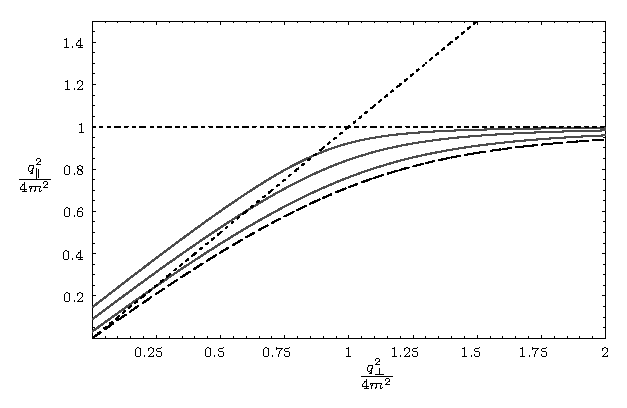
\includegraphics[width = 15cm]{fig2_1.eps}}
	\vspace*{-2mm} \caption{Законы дисперсии фотона моды 2 в сильном магнитном поле  $B/B_e = 200$  
		и нейтральной плазме ($\mu=0$) для различных значений температуры:  $T = 1$ МэВ 
		(верхняя кривая), $T = 0.5$ МэВ (средняя кривая), $T = 0.25$ МэВ (нижняя кривая). 
		Дисперсия фотона без плазмы обозначена штриховой линией.
		Диагональная штриховая линия соответствует вакуумному закону дисперсии, $q^2 = 0$. Угол
		между импульсом фотона  и направлением  магнитного поля равен 
		$\pi/2$. } 
	\label{fig:disT}
\end{figure}

Следует отметить, что полученные собственные векторы~(\ref{eq:r132}) не являются единичными, и для описания поляризационных состояний фотона удобнее использовать нормированные векторы:
%
\beq
\label{eq:epsilon}
%&&
\varepsilon_\alpha^{(1)}(q) = \frac{r^{(1)}_{\alpha}}{\sqrt{|(r^{(1)} r^{*(1)})|}} = 
\frac{(q \varphi)_\alpha}{\sqrt{q_{\mprp}^2}} \, , \quad
%\\
%\nonumber
%&&
\varepsilon_\alpha^{(2)}(q) = \frac{r^{(2)}_{\alpha}}{\sqrt{|(r^{(2)} r^{*(2)})|}} = 
\frac{(q \tilde \varphi)_\alpha}{\sqrt{q_{\mprl}^2}}.
\eeq
\noindent Здесь символы 1 и 2 соответствуют  $\|$ и $\perp$ --  поляризациям в чистом магнитном поле~\cite{Adler:1971}, $X$ - и $O$ -  модам работы~\cite{Mushtukov:2016}, и $E$ - и $O$ -  модам в замагниченной плазме~\cite{Thompson:1996}. 

Нетрудно увидеть, что полученные таким образом собственные векторы и собственные значения поляризационного 
оператора в плазме с точностью до членов порядка  $O(1/\beta^2)$ and $O(\alpha^2)$ совпадают с соответствующими величинами в  замагниченном вакууме~\footnote{Под термином <<замагниченный вакуум>>  понимается магнитное поле без плазмы.}. Такой вывод находится в согласии с результатами работы~\cite{Shabad:1988} и, для предельного случая $\omega \ll m_e$ и после необходимых преобразований: выбора продольной составляющей $\varepsilon^{(2)}_\alpha$ и перехода в систему координат, в которой вектор импульса фотона направлен вдоль оси $z$, работы~\cite{Potekhin:2004}.

Закон дисперсии фотона моды 1 в приближении $O(1/\beta^2)$ практически не отличается от вакуумного, $q^2 \simeq 0$. Действительно, из закона дисперсии для этой моды:
%
\beq
q^2 - {\cal P}^{(1)} = 0 \, 
\label{disper1}
\eeq
\noindent и формулы~(\ref{eq:kappa10}) следует, что
%
\beq
q_{\mprl}^2 = \left (1- \frac{\alpha}{3\pi} \frac{1}{1-\frac{\alpha}{3\pi} \cal V} \right) \, q_{\mprp}^2  
\simeq q_{\mprp}^2 \left (1- \frac{\alpha}{3\pi} \right)\, , 
\label{disper12}
\eeq
\noindent так что $q^2 \simeq 0$, оставаясь при этом отрицательным. Кроме того, из формулы~(\ref{eq:kappa10}) следует, что в кинематической области $q^2_{\mprl} \ll (m_e+\sqrt{m_e^2+2 \beta})^2$ собственное значение поляризационного оператора моды 1 не имеет мнимой части~\footnote{Строго говоря, мнимая часть является сильно подавленной по сравнению с реальной частью, так что такой фотон будет квазистабильным [\textcolor{red}{ссылка}].}

\begin{figure}[t]
	\centerline{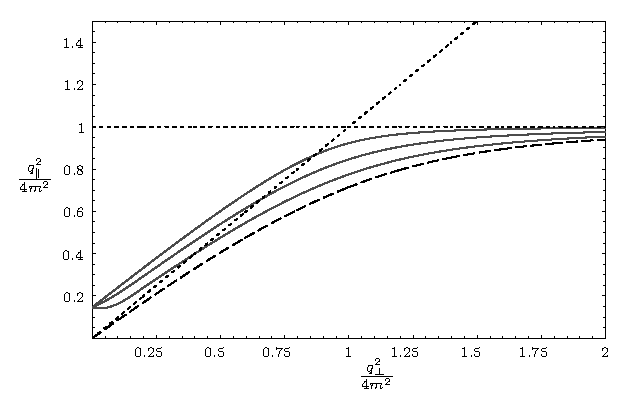
\includegraphics[width=15cm]{fig2_2.eps}} \vspace*{-2mm}
	\caption{Законы дисперсии фотона моды 2 в сильном магнитном поле  $B/B_e = 200$  
		и нейтральной плазме $(T = 1 \mbox{МэВ})$ для различных значений
		угла  между импульсом фотона  и направлением  магнитного поля
		$\theta = \pi/2$ (верхняя кривая), $\theta = \pi/6$  (средняя кривая), $\theta = \pi/12$
		(нижняя кривая).
		Дисперсия фотона без плазмы обозначена штриховой линией.
		Диагональная штриховая линия соответствует вакуумному закону дисперсии, $q^2 = 0$ \textcolor{red}{Заменить на $\mu \neq 0$}.
	}
	\label{fig:disTheta}
\end{figure}

С другой стороны, дисперсионные свойства фотона моды 2  претерпевают существенные изменения даже по сравнению с замагниченным вакуумом и, следовательно, будут оказывать дополнительное влияние на кинематику процессов с участием фотонов этой моды. На рис.~\ref{fig:disT} и~\ref{fig:disTheta} представлены законы дисперсии фотона моды 2 в замагниченной зарядово-симметричной ($\mu=0$) плазме, для различных значений температур, углов и импульса фотона, полученные как решения уравнения
%
\beq
q^2 - {\cal P}^{(2)} = 0 \, .
\label{disper}
\eeq
\noindent Как нетрудно видеть, в противоположность чистому 
магнитному полю, в плазме существует область с  $q^2 > 0$ ниже  первого  
циклотронного резонанса, определяемого условием $q^2_{\mprl} = 4 m_e^2$. 

Этот факт связан  с появлением плазменной частоты в представлении реальных электронов и позитронов среды, 
которая может быть определена из уравнения
%
\begin{equation}
\omega_{pl}^2 - {\cal P}^{(2)} (\omega_{pl}, {\mathbf k} \to 0 ) = 0.
\label{eq:omegapl}
\end{equation}
%
Для случая сильно замагниченной зарядово-симметричной нерелятивистской плазмы можно получить приближенное решение этого уравнения. В результате мы получим классическое выражение $\omega_{pl}^2 \simeq 2(4\pi \alpha n_{e})/m_e$ (множитель 2 возникает из-за равенства концентраций электронов и позитронов), где
%
\begin{eqnarray}
n_{e} \simeq \beta \sqrt{\frac{m_e T}{(2\pi)^3}}\,e^{-m_e/T}.
\label{eq:ne}
\end{eqnarray}
\noindent Таким образом, $\omega_{pl}$ для зарядово-симметричной плазмы экспоненциально подавлено. С другой стороны, для зарядово-несимметричной плазмы подавление отсутствует и $\omega_{pl}^2 \simeq (2\alpha \beta/\pi)v_F$.

Тем не менее, даже для зарядово-симметричной плазмы при температуре $T=50$ кэВ и индукции магнитного поля $B=200 B_e$ мы получаем такую оценку для плазменной частоты: $\omega_{pl} \simeq 3$ кэВ, что уже может повлиять на кинематику различных процессов с участием фотона. Например, наличие плазменной частоты приводит к возникновению порога для каналов рассеяния фотона моды 2 на электронах и позитронах плазмы, $\gamma_2 e \to \gamma_1 e$, $\gamma_2 e \to \gamma_2 e$, который отсутствует в чистом магнитном поле. А для одной из основных реакций, в которых рождаются поляризованные фотоны, -- процесса расщепления фотона на два фотона, $\gamma \to \gamma \gamma$, оно приводит к возникновению новых правил отбора по поляризациям: в области ниже порога рождения $e^+e^-$-пар, $q^2_{\mprl} = 4 m_e^2$, и в области, где $q^2 > 0$, каналы, в которых рождаются фотоны моды 2, $\gamma_2 \to \gamma_2 \gamma_2$,
$\gamma_1 \to \gamma_2 \gamma_2$ и $\gamma_1 \to \gamma_1 \gamma_2$, кинематически закрыты и становится открытым новый канал $\gamma_2 \to \gamma_1 \gamma_1$, запрещенный в магнитном поле в отсутствие плазмы.

Пропагатор фотона определяется решением следующего волнового уравнения:
\begin{eqnarray}\label{eq:WaveEq}
	\nonumber
	&& 
	(g_{\alpha \rho} \, \partial_{\mu}^2  -
	\partial_{\alpha}\partial_{\rho}) \, G^{\rho}_{\phantom{x}\beta}(x) + 
	\int d^4 x'\, {\cal P}^{(\lambda)}_{\alpha\rho} (x - x') \, 
	G^{\rho}_{\phantom{x}\beta}(x)
	\nonumber= g_{\alpha\beta}\delta^4(x),
	\label{eq:2}
\end{eqnarray}
%                                                                                         \frac{(\varphi q)_\mu}{\sqrt{q^2_\perp}}
где $\delta^4(x)=\delta(t)\delta(x)\delta(y)\delta(z)$. 

В координатном пространстве пропагатор фотона можно представить следующим 
образом:
\begin{equation}\label{eq:InvGcFourier}
	G_{\mu\nu}(x)=\int \frac{\dd^4q}{(2\pi)^4}G_{\mu\nu}(q) e^{-\ii qx}\, ,
\end{equation}
где
\begin{equation}\label{eq:GcFourier}
	G_{\mu\nu}(q)=\sum_{\lambda=1}^{3}\frac{b_\mu^{(\lambda)}b^{(\lambda)}_\nu}{(b^{(\lambda)})^2}\cdot
	 \frac{1}{q^2-{\cal P}^{(\lambda)}(q)}
\end{equation}
-- фурье-образ пропагатора.


\label{Ch:Photon}
\section{Резонанс на виртуальном электроне (фермионе)}
\subsection{Комптоновское рассеяние}
Интерес к изучению комптоновского рассеяния $\gamma e \to \gamma e$ в 
сильном магнитном поле первоначально был вызван неожиданным открытием циклотронных 
спектральных линий у двойных рентгеновских 
пульсаров~\cite{Truemper1978,Makishima1990,Grove1995}, которые изначально 
интерпретировались либо как циклотронное поглощение, либо как циклотронное 
излучение~\cite{Truemper1978}. Дальнейшее повышение разрешения детекторов по 
энергии позволило уверенно заключить, что циклотронные особенности связаны 
именно с резонансным поглощением фотона~\cite{Mihara:1990}.
При этом под циклотронным резонансом обычно понимается 
резкое увеличение сечения рассеяния по сравнению с классическим томсоновским 
сечением $\sigma_T = 8 \pi \alpha^2 /(3 m^2)$. В одной из первых 
работ по этой тематике~\cite{Canuto:1971} выражение для сечения 
комптоновского 
рассеяния в магнитном поле без плазмы было получено
в нерелятивистском пределе, и для фотона, 
распространяющегося вдоль магнитного поля, в сечении был обнаружен резонансный 
пик при энергии:
\begin{equation}\label{eq:w_B}
	\omega_B\simeq \frac{\beta}{m}.
\end{equation}
 
Кроме того, в работе~\cite{Canuto:1971} также было показано, что сечение рассеяния фотона 
на электроне
значительно зависит как от поляризационного состояния фотона, так и от угла 
между направлением импульса начального фотона и направлением магнитного поля. В 
последовавшей за ней 
статье~\cite{Gnedin1973} 
исследовалось изменение энергии фотона в комптоновском процессе, кратное 
циклотронной частоте $\omega_B$~(\ref{eq:w_B}). 
В следующих работах~\cite{Borner1979,Ventura:1979} 
были получены результаты для полного сечения рассеяния фотона на электроне с использованием формализма работы~\cite{Canuto:1971}, которые будут справедливыми только для относительно слабого магнитного поля~$B<10^{12}$~Гс. Однако при значениях магнитного поля~$B>10^{12}$~Гс, как было показано в работах~\cite{Herold:1979,Melrose:1983III},   учет релятивистских эффектов в сечении комптоновского рассеяния становится 
существенным.

В представленных выше работах предполагалось, что начальный и конечные электроны находятся 
на основном уровне Ландау, что является справедливым для предела сильного магнитного поля 
и/или низких температур $T\ll m$ (см. Введение). В этом случае резонансный 
пик~(\ref{eq:w_B})  смещается в область более низких энергий фотона, а кроме 
него возникает бесконечный ряд резонансных пиков, соответствующих разным 
уровням Ландау $n$ 
виртуального электрона. Эти пики реализуются при энергиях фотона:
\begin{equation}\label{eq:whn}
	\omega_n(\theta)= \frac{\sqrt{m^2+2 \beta n \sin^2\theta} - 
		m}{\sin^2\theta}\, ,
\end{equation}
где $\theta$ -- угол между импульсом начального фотона и направлением 
магнитного поля. 

С другой стороны, в результате комптоновского процесса могут возбуждаться 
высшие уровни Ландау начального электрона, что, в свою очередь, может выступать 
механизмом рождения фотонов малых энергий для магнитных полей $B\lesssim 
B_e$~\cite{Daugherty:1986,Bussard:1986}. В таком случае для произвольных уровней Ландау $\ell$ начального электрона резонансные 
пики будут наблюдаться на энергиях:
\textcolor{red}{
\begin{equation}\label{eq:resAll}
	\omega_{n\ell}(\theta)=\frac{\sqrt{M_\ell^2 - \sin^2\theta (M_\ell^2-M_n^2)}-M_\ell}{\sin^2\theta}\, ,
\end{equation}}
где $M_\ell=\sqrt{m^2+2\beta \ell}$, $M_n=\sqrt{m^2+2\beta n}$ и т.п.

В рассмотренных выше работах сечение комптоновского рассеяния 
становится бесконечным при энергиях фотона, соответствующих циклотронным 
резонансам~(\ref{eq:whn}) вследствие предположения о 
большом времени жизни виртуальных частиц. По этой причине их результаты 
справедливы только для областей энергий фотона вдали от резонансов
и могут быть применены, например, для моделирования излучения 
	\textcolor{red}{замагниченной 
	холодной плазмы вблизи поверхности нейтронных 
	звезд~\cite{Ozel:2001} или же для относительно слабых магнитных\linebreak полей $B\lesssim 10^{10}$ Гс~\cite{Zavlin:1996}.}

С другой стороны, учет резонансов в комптоновском процессе является необходимым 
при моделировании спектров излучения сильно замагниченных нейтронных 
звезд~\cite{Alexander:1991,Araya:1999,Ho:2001,Lyutikov:2006,Potekhin:2004,Schonherr:2007,Nishimura:2008,Suleimanov:2009}.
Вблизи поверхности нейтронной звезды, где формируется излучение, резонансный 
обратный комптоновский процесс рассеяния фотонов малых энергий на высокоэнергетических электронах 
является доминирующим процессом, который приводит к охлаждению плазмы 
внутренней магнитосферы и образованию высокоэнергетического хвоста в спектре 
излучения~\cite{Fernandez:2007,Nobili:2008,Baring:2018,Beloborodov:2013}.
%Ozel2001: Перенос излучения сильно замагниченой атмосферы НС и конструирование излучательно равновесные модели для спектра. Атмосфера полностью ионизирована с идеальным газом в локальном термодинамическом равновесии. Атмосфера тонкая. 10^13<B<10^15. Предел холодной плазмы.
%Zavlin:1996 Слабые поля для разного химического состава.
%

Вблизи 
циклотронных резонансов для расчета сечения 
комптоновского рассеяния требуется учесть полную 
ширину изменения состояния \linebreak электрона. В нерелятивистском 
пределе~\cite{Canuto:1971} присутствует лишь одна резонансная 
частота~(\ref{eq:whn}) и сечение рассеяния
не зависит от поляризационного состояния электрона (или его спинового состояния), 
поэтому ввести полную ширину относительно просто~\cite{Daugherty:1989}. Однако 
в сильных магнитных полях~$B\gtrsim B_e$ и при высоких энергиях частиц 
требуется учитывать релятивистские поправки, что приводит к тому, что выражение 
для  сечения 
становится очень громоздким, поскольку оно имеет бесконечное число 
резонансов~(\ref{eq:resAll}), 
содержащихся в сумме по всем промежуточным виртуальным состояниям.

Изначально для учета конечных резонансных пиков использовались усредненные по спину ширины распада промежуточного состояния~\cite{Gonthier:2000, Holodov:2000}. 
Как было указано в работе~\cite{Gonthier:2014}, такой подход не является 
точным, поскольку усреднение по спину некорректно учитывает спиновую 
зависимость времени распада виртуального электрона, что приводит к неверному значению сечения комптоновского рассеяния в точке 
резонанса. Этот недостаток был устранен в работе~\cite{Mushtukov:2016}, где 
представлено сечение рассеяния процесса $\gamma e\to \gamma e$ с учетом 
ширины распада виртуальных промежуточных состояний, которая 
зависит от 
поляризационного состояния электрона. 
Однако полное сечение комптоновского рассеяния, полученное таким методом, 
представляет собой громоздкое выражение, что, например, затрудняет его 
использование в моделях переноса излучения. 

В ряде случаев выражение сечения рассеяния можно упростить для получения 
аналитического 
решения различных задач. 
Так, в работе~\cite{Gonthier:2000} была использована 
аппроксимация сечения рассеяния с учетом резонанса в ультрарелятивистском 
пределе для случая относительно сильного магнитного поля $B>0.1 B_e$. В точке 
циклотронного резонанса виртуальный электрон становится реальным и распадается 
на масштабе комптоновского времени, поэтому вероятность
комптоновского рассеяния сводится к вероятности одновершинного процесса 
поглощения фотона электроном $\gamma 
e \to e$. В 
работе~\cite{Harding:1991} исследовался вопрос аппроксимации комптоновского 
сечения с помощью одновершинного процесса поглощения фотона электроном для 
магнитных полей 
$B\sim 
0.1B_e$. При этом различие между одновершинным процессом поглощения и комптоновским 
рассеянием становится существенным на высших циклотронных резонансах из-за 
нерезонансного вклада. Еще один подход рассмотрен в 
работе~\cite{Rumyantsev:2017}, он заключается в том, что пропагатор 
виртуального электрона можно заменить 
на дельта-функцию, когда основной вклад 
в сечение рассеяния будут давать области вблизи резонансов (приближение узкого 
пика). 
 
Далее рассмотрим получение сечения рассеяния комптоновского процесса в случае узкого резонансного пика.
Лагранжиан взаимодействия электрона с фотоном может быть представлен в виде:
%
\begin{eqnarray}\label{eq:L}
	{\cal L}(X) \, = \,- e [\bar \Psi_f (X) \gamma^{\mu} A^{(\lambda)}_\mu (X) \Psi_f(X)] \, ,
	\label{eq:Lel}
\end{eqnarray}
%
\noindent где $\gamma^{\mu}$ -- гамма-матрицы Дирака, а волновые функции электрона, $\Psi_f (X)$, и фотона, $A^{(\lambda)}_\mu (X)$, были введены в предыдущих разделах.

$S$-матричный элемент рассеяния фотона поляризации $\lambda$ на электроне с рождением электрона и фотона поляризации $\lambda'$, с учетом лагранжиана~(\ref{eq:L}) может быть представлен в виде:  
%
\beq                          
\nonumber
S^{s^{\, \prime} s}_{\gamma^{(\lambda)} e \to \gamma^{(\lambda')} e'} &=& - e^2\int \dd^4 X \dd^4 Y A^{(\lambda)}_\mu (X) A^{(\lambda')}_{\mu'} (Y)
%\times 
%\\[3mm]
%\nonumber
%&\times& 
\, \left [\bar \Psi^{s'}_{p',\ell'}(Y) \gamma_{\mu'} 
S^{s''}_n (Y,X) 
\gamma_\mu \Psi^{s}_{p,\ell}(X) \right ]\, +
\\[3mm]
\label{eq:S1a}
&+& (A^{(\lambda)}_\mu, \gamma_\mu \leftrightarrow A^{(\lambda')}_{\mu'}, \gamma_{\mu'})\, .
\eeq

Если в области резонанса выполняется условие $P_0\Gamma^{s''}_n\ll \left|P^2\mprl-M_n^2\right|$, тогда квадрат знаменателя пропагатора может быть заменен на $\delta$-функцию:
\begin{equation}
	\label{gamma_factor}
	\left|\frac{1}{P^2_{\mprl}-M_n^2-\ii P_0\Gamma^{s''}_n/2}\right|^2
	\simeq\frac{2\pi}{P_0\Gamma_n^{s''}} \delta(P^2_{\mprl}-M_n^2).
\end{equation}
%
С учетом этого квадрат $S$-матричного элемента, определяющий вероятность процесса и необходимый при расчетах вычисляемых величин, таких как сечение рассеяния, может быть представлен в факторизованном виде:
%
\beq
\label{eq:S2factor1}
\sum\limits_{s, s' = \pm 1} \frac{|{\cal S}^{s^{\,\prime} s}_{{\gamma^{(\lambda)} e_\ell \to \gamma^{(\lambda')} e_{\ell'}}}|^2}{\tau} = 
\sum\limits_{s, s', s'' = \pm 1} 
\sum\limits_{n=0}^{\infty} \;  \int \frac{\dd p^{\, \prime \prime}_y 
	\dd p^{\, \prime \prime}_z}{(2 \pi)^2 \; \Gamma_n^{s''}} \,  
\frac{|{\cal S}^{s^{\,\prime \prime} s}_{\gamma^{(\lambda)} e_\ell \to e_n}|^2}{\tau} \, 
\frac{|{\cal S}^{s^{\,\prime} s''}_{ e_n \to \gamma^{(\lambda')} e_{\ell'}}|^2}{\tau} \, ,
\eeq
%
где 
\beq
%\nonumber
\label{eq:Sjf}                                  
{\cal S}^{s^{\,\prime \prime} s}_{\gamma^{(\lambda)} e_\ell \to e_n} = 
\frac{\ii (2\pi)^3 
	\delta^{(3)}_{0,y,z} (P - p^{\, \prime \prime})}
{\sqrt{2q_0 V 2 E_{\ell} L_y L_z 2 E^{''}_{n} L_y L_z}}\, 
{\cal M}^{s'' s}_{\gamma^{(\lambda)} e_\ell \to e_n} \, ,
\\
\nonumber
S_{e_n \to \gamma^{(\lambda')} e_{\ell'}}=S_{\gamma^{(\lambda)} e_\ell \to e_n}(q\to q', E_\ell \to E'_{\ell'}) \, 
\eeq
%
\noindent-- $S$-матричные элементы подпроцессов: поглощения фотона, $e\gamma \to e$, и рождения фотона, $e \to e\gamma$.

Амплитуда ${\cal M}^{s'' s}_{\gamma^{(\lambda)} e_\ell \to e_n}$ одновершинного процесса записывается следующим образом:
%
\beq
\label{eq:amplonever} 
{\cal M}^{s'' s}_{\gamma^{(\lambda)} e_\ell \to e_n} =  \frac{\exp{[-\ii q_x (p_y + p_y^{\,\prime \prime})/(2\beta)]}}{\sqrt{M_{\ell} M_n (M_{\ell} + m) 
		(M_n + m)}} 
\left [ \frac{q_y+\ii q_x}{\sqrt{q_{\mprp}^2}} \right ]^{n-\ell} {\cal T}^{s'' s}_{V} \, ,
\eeq

${\cal T}^{s'' s}_{V}$ выражаются через  
лоренц-коварианты и инварианты~  в подпространстве~$\{0, 3\}$:

\begin{equation}
	\label{eq:K1}
	{\cal K}_{1\alpha} = \sqrt{\frac{2}{(p\widetilde \Lambda p^{\, \prime \prime}) + 
			M_\ell M_{n}}} \left \{M_\ell (\widetilde \Lambda p^{\, \prime \prime})_\alpha + 
	M_{n} (\widetilde \Lambda p)_\alpha  \right \}\, ,
\end{equation}
%
\begin{equation}
	{\cal K}_{2\alpha} = \sqrt{\frac{2}{(p\widetilde \Lambda p^{\, \prime \prime}) + 
			M_\ell M_{n}}} \left \{M_\ell (\widetilde \varphi p^{\, \prime \prime})_\alpha + 
	M_{n} (\widetilde \varphi p)_\alpha  \right \}\, ,
	\label{eq:K2}
\end{equation}

\begin{equation}
	\label{eq:K3}
	{\cal K}_{3} = \sqrt{2\left [(p\widetilde \Lambda p^{\, \prime \prime}) + 
		M_\ell M_{n} \right]} \, ,  
\end{equation}
%
\begin{equation}
	\label{eq:K4}
	{\cal K}_4 = 
	- \sqrt{\frac{2}{(p\widetilde \Lambda p^{\, \prime \prime}) + M_\ell M_{n}}}\, 
	(p\widetilde \varphi p^{\, \prime \prime}) \, .
\end{equation}

для $n \geqslant \ell$
%
\begin{eqnarray}
	\nonumber
	&&{\cal I}_{n, \ell} (x) = \sqrt{\frac{\ell !}{n !}} \; \eee^{-x/2} x^{(n-\ell)/2} L_\ell^{n-\ell} (x) \, ,
	\\
	&&{\cal I}_{\ell, n} (x) = (-1)^{n-\ell} {\cal I}_{n, \ell} (x) \, ,
	\label{eq:Inl}
\end{eqnarray}
\noindent и $L^k_n (x)$ -- обобщенные полиномы Лагерра~\cite{Gradstein:1963}.
Далее в работе будет использовано обозначение ${\cal I}_{n, \ell}\equiv{\cal I}_{n, \ell} \left(\frac{q_\perp^2}{2\beta}\right)$ и для определенности рассматриваются электроны, для которых знак заряда $\eta=-1$.

\begin{eqnarray}
\nonumber
&&{\cal T}^{--}_V  = g_V [ 2\beta\sqrt{\ell n} ({\cal K}_1 \varepsilon^{(\lambda)}) {\cal I}_{n-1,\ell-1} +
(m_f+M_\ell)(m_f+M_n)\times
\\[3mm]
\label{V--}
&&\times({\cal K}_1 \varepsilon^{(\lambda)}) {\cal I}_{n,\ell} -
\sqrt{2\beta n} (m_f+M_\ell) {\cal K}_3 \frac{(\varepsilon^{(\lambda)}\Lambda q) - 
\ii (\varepsilon^{(\lambda)} \varphi q)}{\sqrt{q^2_{\mprp}}} {\cal I}_{n-1,\ell} -
\\[3mm]
\nonumber
&& - \sqrt{2\beta \ell} (m_f+M_n) {\cal K}_3 
\frac{(\varepsilon^{(\lambda)}\Lambda q) + \ii (\varepsilon^{(\lambda)}\varphi q)}{\sqrt{q^2_{\mprp}}} {\cal I}_{n,\ell-1}] \, ;
\end{eqnarray}
%
\begin{eqnarray}
\nonumber
&&{\cal T}^{-+}_V = \ii g_V [\sqrt{2\beta n} (m_f+M_\ell) ({\cal K}_2 \varepsilon^{(\lambda)}) 
{\cal I}_{n-1,\ell-1} - 
 \sqrt{2\beta \ell} (m_f+M_n) \times
\\[3mm]
\label{eq:tV-+}
%transversal
&&\times  ({\cal K}_2 \varepsilon^{(\lambda)}) 
{\cal I}_{n,l} + 2\beta\sqrt{\ell n} {\cal K}_4 
\frac{(\varepsilon^{(\lambda)}\Lambda q) - \ii (\varepsilon^{(\lambda)} \varphi q)}{\sqrt{q^2_{\mprp}}} {\cal I}_{n-1,\ell} -
\\[3mm]
\nonumber
&&- (m_f+M_\ell)(m_f+M_n) {\cal K}_4 
\frac{(\varepsilon^{(\lambda)}\Lambda q) + \ii (\varepsilon^{(\lambda)}\varphi q)}{\sqrt{q^2_{\mprp}}} {\cal I}_{n,\ell-1}]  \, ;
\end{eqnarray}
%
\begin{eqnarray}
\nonumber
&&{\cal T}^{+-}_V = -\ii g_V [\sqrt{2\beta \ell} (m_f+M_n) ({\cal K}_2 \varepsilon^{(\lambda)}) 
{\cal I}_{n-1,\ell-1} - 
 \sqrt{2\beta n} (m_f+M_\ell) \times
\\[3mm]
\label{eq:tV+-}
%transversal
&&\times  ({\cal K}_2 \varepsilon^{(\lambda)}) 
{\cal I}_{n,\ell} + (m_f+M_\ell)(m_f+M_n) {\cal K}_4 
\frac{(\varepsilon^{(\lambda)}\Lambda q) - \ii (\varepsilon^{(\lambda)} \varphi q)}{\sqrt{q^2_{\mprp}}} {\cal I}_{n-1,\ell} -
\\[3mm]
\nonumber
&&- 2\beta\sqrt{\ell n} {\cal K}_4 
\frac{(\varepsilon^{(\lambda)}\Lambda q) + \ii (\varepsilon^{(\lambda)} \varphi q)}{\sqrt{q^2_{\mprp}}} {\cal I}_{n,\ell-1}]  \, ;
\end{eqnarray}
%
\begin{eqnarray}
\nonumber
&&{\cal T}^{++}_V  = g_V [2\beta\sqrt{\ell n} ({\cal K}_1 \varepsilon^{(\lambda)}) {\cal I}_{n,\ell} +
 (m_f+M_\ell)(m_f+M_n) ({\cal K}_1 \varepsilon^{(\lambda)}) \times
\\[3mm]
\label{eq:tV++} 
%transversal
&&\times  {\cal I}_{n-1,\ell-1} - \sqrt{2\beta \ell} (m_f+M_n) {\cal K}_3 
\frac{(\varepsilon^{(\lambda)}\Lambda q) - \ii (\varepsilon^{(\lambda)}\varphi q)}{\sqrt{q^2_{\mprp}}} {\cal I}_{n-1,\ell} -
\\[3mm]
\nonumber
&&- \sqrt{2\beta n} (m_f+M_\ell) {\cal K}_3 
\frac{(\varepsilon^{(\lambda)}\Lambda q) + \ii (\varepsilon^{(\lambda)} \varphi q)}{\sqrt{q^2_{\mprp}}} {\cal I}_{n,\ell-1}] \, .
\end{eqnarray}










Для астрофизических приложений полученных результатов удобно вместо сечения использовать коэффициент поглощения фотона -- вероятность перехода фотона в другое состояние за счёт тех или иных процессов, который для комптоновского процесса был определен, например, в работе~\cite{Chistyakov:2009}:
\begin{eqnarray}\label{eq:WabsStrongB}
	&&W_{\gamma^{(\lambda)} e \to \gamma^{(\lambda')} e} = \frac{\beta}{16 (2\pi)^4
		\omega_{\lambda}}
	\int \mid {{\cal M}^{s'' s}_{\gamma^{(\lambda)} e_\ell \to \gamma^{(\lambda')} e_{\ell'}}}\mid^2 \times
	\label{eq:Wscatt}\\
	&&\times f_{E}\, [1-f_{E'}] \, (1 + f_{\omega'})
	\delta (\omega_{\lambda}({\bf k}) + E - \omega_{\lambda^{'}}({\bf k'}) - E')
	\frac{dp_z\,d^3 k^{'}}{ E E' \omega_{\lambda^{'}}},
	\nonumber
\end{eqnarray}
где $f_{E}=(1+\exp[E/T])^{-1}$ -- равновесная функция распределения электронов с температурой $T$ и нулевым химическим потенциалом, \mbox{$f_\omega=(\exp[E/T]-1)^{-1}$} -- равновесная функция распределения фотонов. С помощью коэффициента поглощения удобно, например, вычислять длину свободного пробега \mbox{$\ell_\lambda=W^{-1}_{\gamma^{(\lambda)} e\to \gamma e}$}, а дифференциальный коэффициент поглощения входит в уравнение Больцмана.


Подставляя факторизованные квадраты амплитуд~(\ref{eq:delta_f}) с учетом\linebreak (\ref{eq:S2factor})--(\ref{eq:amplonever}) в выражение~(\ref{eq:WabsStrongB}), суммируя по поляризационным состояниям конечного электрона и фотона и проводя несложное интегрирование, получим:

\beq
\label{eq:wabs1} 
&&W_{\gamma^{(1)} e \to \gamma e} = \frac{\alpha \beta}{2 \omega} 
\sum \limits^{\infty}_{\ell=0}  \sum \limits^{\infty}_{n=n_{0}} \sum \limits_{\epsilon = \pm 1} 
%\times 
%\\
%\nonumber
%&&\times 
\frac{f_{-}(E^{\epsilon}_{\ell}) [1 - f_{-}(E^{\epsilon}_{\ell} + \omega)]}{\sqrt{(M_n^2-M_{\ell}^2-q^{2}_{\mprl})^2-4 q^{2}_{\mprl}M_{\ell}^2}}
\times 
\\
\nonumber
&&\times 
\bigg \{ [2 \beta (n+\ell) - q^{2}_{\mprl}] ({\cal I}^2_{n,\ell-1}+{\cal I}^2_{n-1,\ell}) - 
%\\
%\nonumber
%&& -
8 \beta \sqrt{\ell n} {\cal I}_{n,\ell-1} {\cal I}_{n-1,\ell} \bigg \}   \, ,
\eeq
%

\beq
\label{eq:wabs2} 
&&W_{\gamma^{(2)} e \to \gamma e} = \frac{\alpha \beta}{2 \omega} 
\sum \limits^{\infty}_{\ell=0}  \sum \limits^{\infty}_{n=n_{0}} \sum \limits_{\epsilon = \pm 1} 
%\times 
%\\
%\nonumber
%&&\times 
\frac{f_{-}(E^{\epsilon}_{\ell}) [1 - f_{-}(E^{\epsilon}_{\ell} + \omega)]}{\sqrt{(M_n^2-M_{\ell}^2-q^{2}_{\mprl})^2-4 q^{2}_{\mprl}M_{\ell}^2}}
\times 
\\
\nonumber
&&\times 
\bigg \{ \left [\frac{(2\beta (n-\ell))^2}{q^{2}_{\mprl}} - 2 \beta (n+\ell) - 4 m^2 \right ] 
%\times 
%\\
%\nonumber
%&& \times 
({\cal I}^2_{n,\ell}+{\cal I}^2_{n-1,\ell-1}) -
\\
\nonumber
&&
-8 \beta \sqrt{\ell n} {\cal I}_{n,\ell} {\cal I}_{n-1,\ell-1} \bigg \}   \, ,
\eeq
где
\beq
\nonumber
&&E^{\epsilon}_{\ell} = \frac{1}{2 q^2_{\mprl}} \, \bigg [\omega \left (M^2_n - M^2_{\ell} - q^2_{\mprl} \right ) + 
\epsilon k_z 
\sqrt{\left (M^2_n - M^2_{\ell} - q^2_{\mprl} \right )^2 - 4 q^2_{\mprl} M^2_{\ell}} \, \bigg ] \, .
\eeq
\noindent В~(\ref{eq:wabs1}) и~(\ref{eq:wabs2}) 
суммирование по $n$ ограничено согласно закону сохранения энергии и импульса следующим образом:  
%
\beq
n_0 = \ell + \left [\frac{q^2_{\mprl} + 2 M_\ell \sqrt{q^2_{\mprl}}}{2 \beta} \right ] \, , 
\eeq
\noindent где $[x]$ -- целая часть числа $x$.

C дифференциальным сечением рассеяния коэффициент поглощения связан следующим 
образом~\cite{Landau:2002}
\begin{equation}
	d\sigma_{\gamma^{(\lambda)} e\to \gamma e}= \frac{dW_{\gamma^(\lambda) e \to \gamma e}}{j},
\end{equation}
\noindent где $j=|(pq)_{\mprl}|/(E \omega V)$ -- плотность потока падающих 
частиц  в продольном по отношению к магнитному полю подпространстве.
В работах~\cite{Mushtukov:2016,Harding:1991,Schwarm:2017} исследовался процесс 
комптоновского рассеяния в замагниченной плазме при ненулевых температурах и 
магнитных полях, характерных 
для магнитосфер радиопульсаров и магнитаров $10^{12}-10^{15}$ Гс. В данных 
работах рассчитано сечение рассеяния при условии, что начальный и конечный 
электроны находятся на основном уровне Ландау. При расчетах учитывался резонанс 
на виртуальном электроне с конечной шириной, полученной с использованием 
корректных решений уравнения Дирака~(\ref{eq:psie}).


В данных работах сечение интегрируется по импульсам начального 
электрона в системе покоя плазмы
с нормированной функцией распределения $\overline{f}_{n,s}(p_z)$:
\begin{equation}\label{eq:dsigma}
	\sigma^*_\lambda=\int_{-\infty}^{\infty} 
	\overline{f}_{n,s}(p_z)\dd\sigma_{\gamma^{(\lambda)} e\to \gamma e}\, ,
\end{equation}
где 
\begin{equation}
	d\sigma_{\gamma^{(\lambda)} e\to \gamma e}= \frac{dW_{\gamma^{(\lambda)} e \to \gamma e}}{j},
\end{equation}
$j=|(pq)_{\mprl}|/(E \omega V)$ -- плотность потока падающих 
частиц  в продольном по отношению к магнитному полю подпространстве. Исходя из 
нормировки функции распределения:
\begin{equation}
	\sum_{n,s}\int_{-\infty}^{\infty} \dd p_z \overline{f}_{n,s}(p_z)=1,
\end{equation}
представим её в виде:
\begin{equation}
	\overline{f}_{n,s}(p_z)=\frac{\beta}{(2\pi)^2n_e}\frac{1}{e^{E_n/T}+1},
\end{equation}
где 
\begin{equation}\label{eq:ne}
	n_e = \frac{\beta}{(2 \pi)^2} \sum \limits^{\infty}_{\ell=0} 
	(2-\delta_{\ell,0}) \int \limits^{\infty}_{-\infty}\dd p_z f_{-}(E_{\ell})
\end{equation}
-- концентрация электронов во внешнем магнитном поле.

С учетом (\ref{eq:dsigma}) -- (\ref{eq:ne}) дифференциальное сечение рассеяния, просуммированное по 
поляризациям конечного фотона, может быть выражена через дифференциальный 
коэффициент поглощения:
\begin{equation}
	d\sigma^*_\lambda=\frac{E\omega}{(pq)_{\mprl}}\frac{1}{n_e} 
	dW_{\gamma^{(\lambda)} e\to\gamma e}\, .
\end{equation}

Следует отметить, что для дифференциального коэффициента поглощения, будучи 
проинтегрировано по импульсам 
начального 
электрона, в 
нерелятивистском пределе переходит в известное классическое соотношение~\cite{Landau:1989}:
\begin{equation}
W_{\gamma^{(\lambda)} e\to\gamma e}=\frac{1}{\ell_\lambda}=n_e 
\sigma_{\gamma^{(\lambda)} e\to\gamma e}\, .
\end{equation}


Согласно раздела~\ref{Ch:Propagator} для рассматриваемых параметров магнитного поля и плазмы, можно считать, что закон дисперсии как моды 1, так и моды 2, в пренебрежении $\omega_{pl}$, мало отличается от вакуумного за исключением точек резонансов. В таком случае параллельную магнитному полю компоненту импульса фотона можно положить
$q_z \simeq \omega \sin{\theta}$, где 
$\theta$ -- угол между импульсом фотона и направлением магнитного поля. Как уже отмечалось в разделе~\ref{Ch:Propagator}, перенормировка волновых функций фотонов становится существенной вблизи циклотронных резонансов $q^2_{\mprl} \simeq (M_n+M_{\ell})^2$, однако, как показывает анализ, при значении магнитного поля $B\simeq 10^{12}$ Гс она становится несущественной так, что~$Z_{1,2}\simeq 1$. 

Сравнительный анализ усредненного сечения по поляризациям начального фотона
\begin{equation}
	\sigma^*=\frac{\sigma^*_{1}+\sigma^*_{2}}{2}
\end{equation}
в единицах $\sigma_T$ с результатами работы~\cite{Harding:1991} для различных значений магнитного поля (\mbox{$B=0.039B_e\simeq1.7\times10^{12}$ Гс и $B=0.23B_e\simeq10^{13}$ Гс}) и температур ($T=5$ кэВ и $T=50$ кэВ) представлен на~рисунках \ref{fig:CompAndHardO}. Полученные результаты показывают, что дельта-функциональное приближение достаточно хорошо описывает резонансные пики. В области резонанса сечение комптоновского рассеяния в данном приближении ожидаемо превышает сечение с учетом конечной ширины, так как знаменатель пропагатора электрона во всей резонансной области при дельта-функциональном приближении всегда дает максимальный вклад в интеграл. С увеличением температуры, помимо уширения резонансных пиков, также наблюдается уменьшение точности дельта-функционального приближения особенно для малых углов между направлением распространения фотона и магнитного поля. При уменьшении магнитного поля наблюдается смещение резонансных пиков, согласно формуле~\ref{eq:whn}, а также их сужение при сохранении формы. Это связано с тем, что энергетические уровни Ландау становятся ближе друг к другу, что приводит к более узким резонансам.   Сравнение сечения комптоновского процесса при различных магнитных полях показывает, что резонансные пики, наблюдаемые при энергиях фотона, соответствующих высшим уровням Ландау виртуального электрона $n>0$, убывают быстрее с ростом энергии для относительно малых магнитных полей.

Как было указано выше, использование дельта-функционального приближения упрощает и ускоряет численный анализ, поэтому представляет интерес, используя приближение узкого резонансного пика, исследовать сечение рассеяния с учетом того, что начальный электрон может занимать произвольный уровень Ландау. Как показал численный анализ, для температуры $T=5$ кэВ и магнитного поля $B\simeq10^{12}-10^{13}$ Гс сечение комптоновского рассеяния с учетом высших уровней Ландау начального электрона лишь незначительно модифицируется, поэтому можно уверенно предполагать, что начальные электроны занимают преимущественно основной уровень Ландау. С другой стороны, при температуре $T\simeq50$ кэВ и магнитном поле~$B\simeq 10^{13}$ Гс, как показано на рисунке~\ref{fig:HardingManyLevels}, учет ненулевых уровней Ландау приводит к существенному увеличению значений сечения в области резонанса. К ещё большим ошибкам (приблизительно на порядок)  будет приводить предположение только основного уровня Ландау начального электрона для малых значений магнитного поля~$B\simeq1.7\times10^{12}$ при той же температуре $T\simeq50$ кэВ.  Как следствие, при малых магнитных полях и высоких температурах учет высших уровней Ландау становится важным аспектом при изучении комптоновского рассеяния в плазме. Также в сечении присутствуют узкие максимумы, известные в литературе (см., например,~\cite{Pavlov:1991,Klepikov:1954,Baier:2007}), соответствующие энергиям $\omega_{n\ell}=(M_n-M_\ell)/\sin \theta$, которые наиболее ярко выражены для фотонов, распространяющихся поперек магнитного поля (см.~ рис.~\ref{fig:HardingManyLevels}), но~вносят малый вклад в интегральные величины.

Представляет интерес исследовать сечение рассеяния с учетом того, что конечный электрон может занимать произвольный уровень Ландау. Для температуры $T=5$ кэВ можно уверенно предполагать, что начальные электроны занимают основной уровень Ландау, так как они практически не вносят вклад в сечение рассеяния. С другой стороны, при температуре $T=50$ кэВ, как показано на рисунках~\ref{fig:HardingManyLevels}, сечение в области резонанса увеличивается и ширина резонаного пика возрастает. Также в сечении присутствуют узкие максимумы, известные в литературе 
%(см., например,~\cite{Pavlov:1991,Klepikov:1954,Baier:2007})
, соответствующие энергиям $\omega_{n\ell}=(M_n-M_\ell)/\sin \theta$, которые наиболее ярко проявляются для фотонов, распространяющихся поперек магнитного поля, но вносят малый вклад в интегральные величины.


\begin{figure}[t!]\centering
	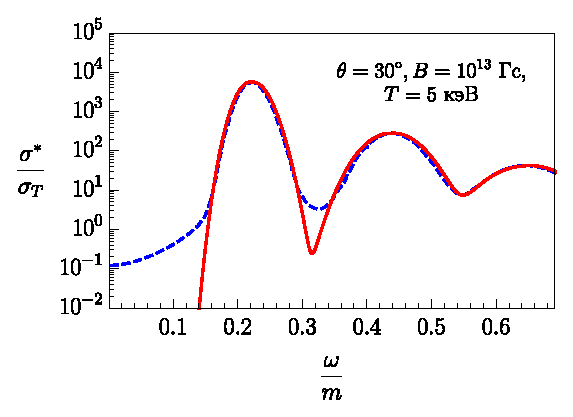
\includegraphics[width=0.32\linewidth,clip]{AliceDeltaAverageB023T001Deg30.eps}
	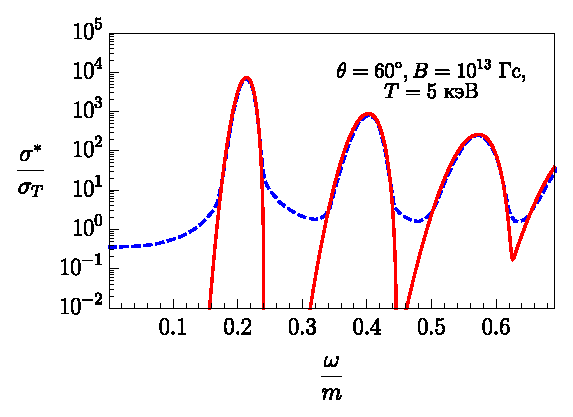
\includegraphics[width=0.32\linewidth,clip]{AliceDeltaAverageB023T001Deg60.eps}
	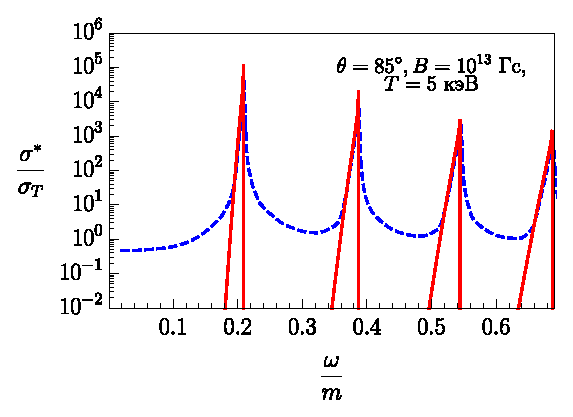
\includegraphics[width=0.32\linewidth,clip]{AliceDeltaAverageB023T001Deg85.eps}
	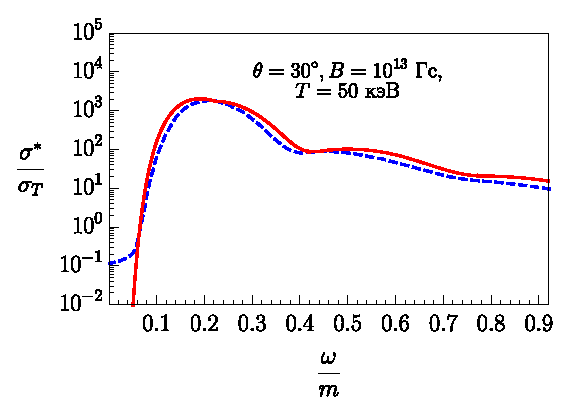
\includegraphics[width=0.32\linewidth,clip]{AliceDeltaAverageB023T01Deg30.eps}
	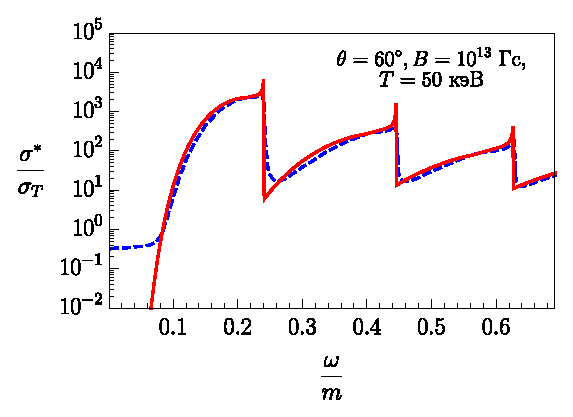
\includegraphics[width=0.32\linewidth,clip]{AliceDeltaAverageB023T01Deg60.eps}
	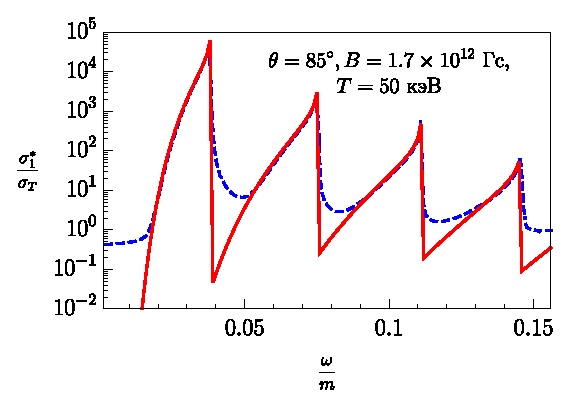
\includegraphics[width=0.32\linewidth,clip]{AliceDeltaAverageB023T01Deg85.eps}
	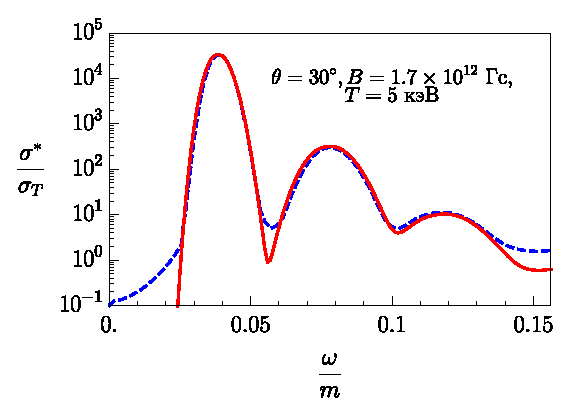
\includegraphics[width=0.32\linewidth,clip]{AliceDeltaAverageB0039T001Deg30.eps}
	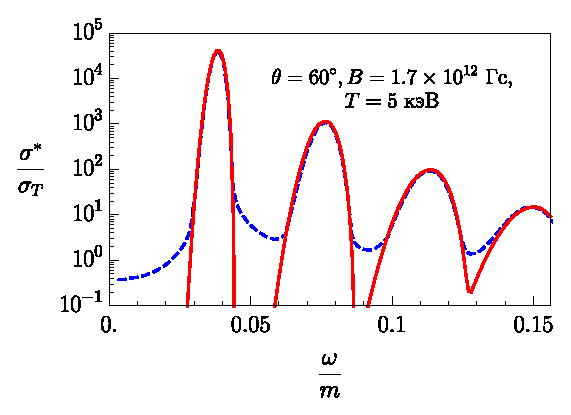
\includegraphics[width=0.32\linewidth,clip]{AliceDeltaAverageB0039T001Deg60.eps}
	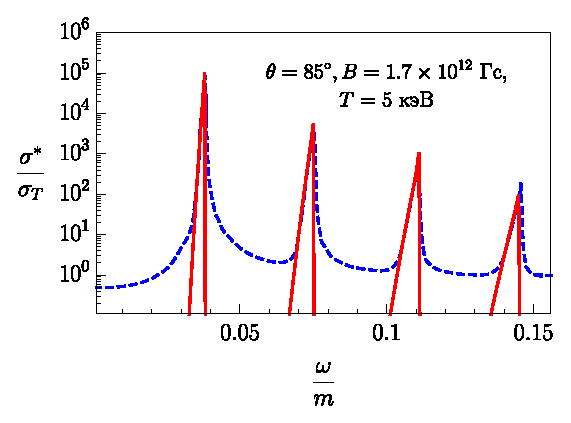
\includegraphics[width=0.32\linewidth,clip]{AliceDeltaAverageB0039T001Deg85.eps}
	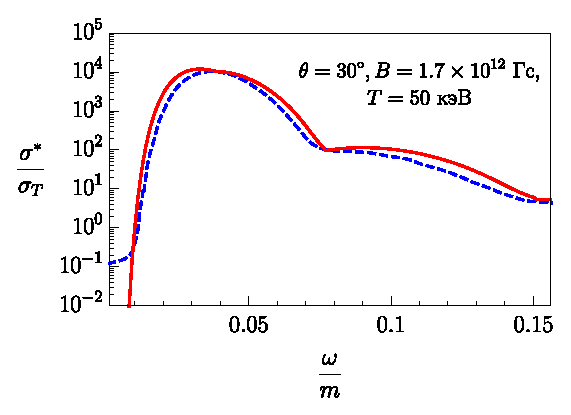
\includegraphics[width=0.32\linewidth,clip]{AliceDeltaAverageB0039T01Deg30.eps}
	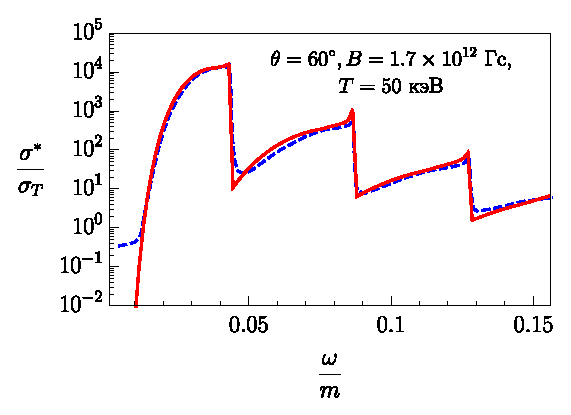
\includegraphics[width=0.32\linewidth,clip]{AliceDeltaAverageB0039T01Deg60.eps}
	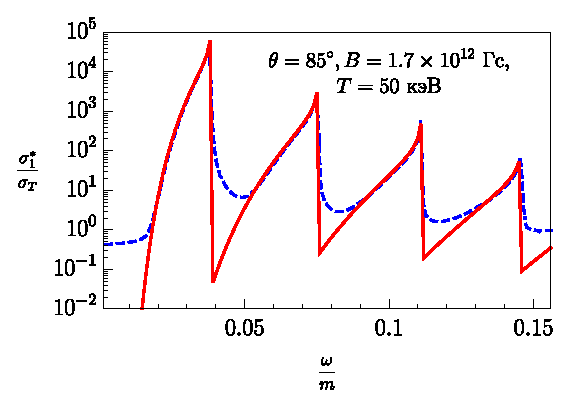
\includegraphics[width=0.32\linewidth,clip]{AliceDeltaAverageB0039T01Deg85.eps}	
	\caption{Cечения (в единицах $\sigma_T$), усредненного по поляризациям начального фотона, $e\gamma^{(2)}  \to e\gamma$, полученном в работе~\cite{Harding:1991} (пунктирная линия) и $\delta$-функциональном приближении (сплошная линия) для различных углов $\theta$ между импульсом фотона и направлением магнитного поля. Все начальные и конечные электроны находятся на основном уровне Ландау.}
	\label{fig:CompAndHardO}
\end{figure}
\clearpage
\begin{figure}[t!]\centering
	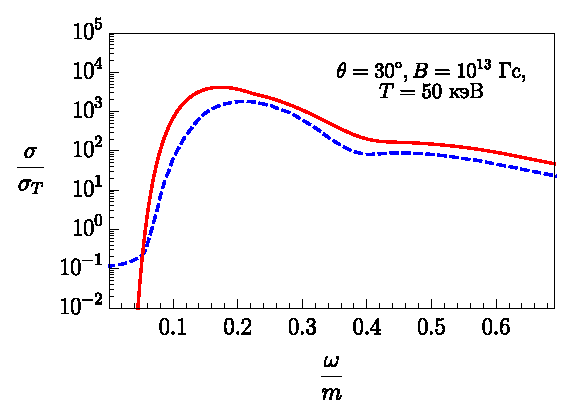
\includegraphics[width=0.55\linewidth,clip]{AliceDeltaManyLevelB023T01Deg30.eps}\\
	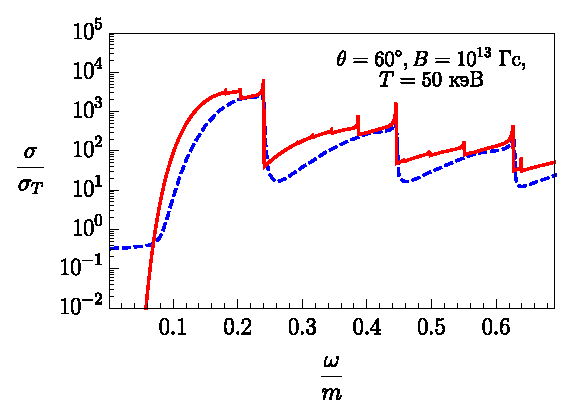
\includegraphics[width=0.55\linewidth,clip]{AliceDeltaManyLevelB023T01Deg60.eps}\\
	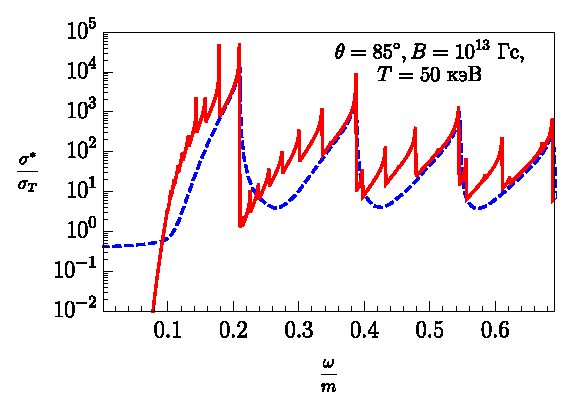
\includegraphics[width=0.55\linewidth,clip]{AliceDeltaManyLevelB023T01Deg85.eps}
	\caption{Cечения (в единицах $\sigma_T$), усредненного по поляризациям начального фотона и по поляризациям начального электрона, $e\gamma^{(2)}  \to e\gamma$, полученном в работе~\cite{Harding:1991} (пунктирная линия) и $\delta$-функциональном приближении (сплошная линия) для различных углов $\theta$ между импульсом фотона и направлением магнитного поля. По начальным электронам взя. Значение температуры $T=50$ кэВ, а индукция магнитного поля -- $B=10^{13}$ Гс.\label{fig:HardingManyLevels}}
\end{figure}
\clearpage
Отметим, что сечение с учетом вклада конечной ширины поглощение электрона, которое было взято непосредственно из результатов работы~\cite{Mushtukov:2016}, имеет завышенные значения по сравнению с дельта-функциональным приближением более чем на 2 порядка во всей области энергий фотона моды 1, за исключением тех случаев, когда фотоны с энергиями вблизи резонанса распространяются поперек магнитного поля~(см.~рис.~\ref{fig:CompAndMushXGround}).  С другой стороны в сечении для фотона моды 2 наблюдаются существенно завышенные значения приблизительно на порядок для углов $\theta=90^\circ$ и $\theta=60^\circ$ между направлением импульса фотона и направлением магнитного поля~(см.~рис.~\ref{fig:CompAndMushO}). Однако сравнительный численный анализ сечения комптоновского рассеяния полученного в работе~\cite{Mushtukov:2016} произведенный в~\cite{SchwarmD:2017} показал, что указанная выше разница отсутствует. При~этом результаты работы~\cite{SchwarmD:2017} находятся в хорошем соответствии с результатами настоящей статьи (см. рис.~\ref{fig:CompAndHardO}), результатами работы~\cite{Harding:1986}, а также более ранней работой~\cite{Mushtukov:2015}, поэтому наличие существенных различий в результатах работы~\cite{Mushtukov:2016} и настоящей диссертации может быть связано с опечатками при построении графиков в~\cite{Mushtukov:2016}.

Таким образом, применение 
приближения~(\ref{eq:delta_f}) правомочно  в области полей $B \sim 10^{12}-10^{15}$ Гс, характерных для магнитаров и радиопульсаров. С другой стороны, полученные коэффициенты поглощения фотона~(\ref{eq:wabs1}) и~(\ref{eq:wabs2}) определяются только как сумма конечных выражений (за исключением особенных точек, указанных ранее), что является гораздо более удобным в приложениях (например, к решению задачи переноса излучения), чем точный учет конечной ширины.
\clearpage
\begin{figure}[t!]\centering
	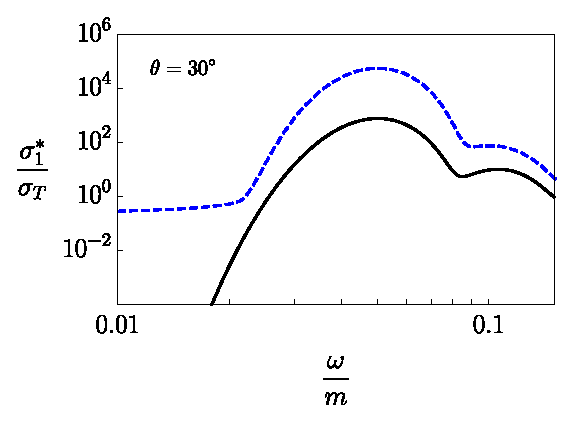
\includegraphics[width=0.5\linewidth,clip]{CompareMushOs005MushtukovX1Ground.eps}
	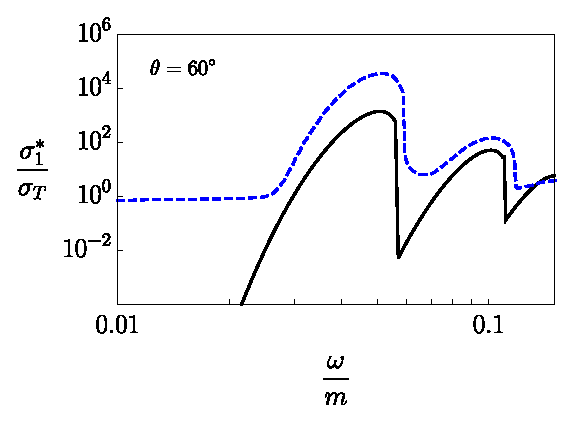
\includegraphics[width=0.5\linewidth,clip]{CompareMushOs005MushtukovX2Ground.eps}
	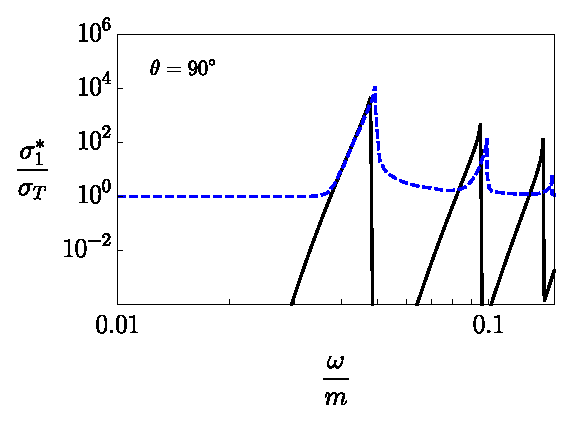
\includegraphics[width=0.5\linewidth,clip]{CompareMushOs005MushtukovX3Ground.eps}
	\caption{Cечения (в единицах $\sigma_T$) рассеяния фотона моды 1, $e\gamma^{(1)}  \to e\gamma$, полученном в работе~\cite{Mushtukov:2016} (пунктирная линия) и $\delta$-функциональном приближении (сплошная линия) для различных углов $\theta$ между импульсом начального фотона и направлением магнитного поля (значения изображены на графиках). $B=2.2\times 10^{12}$ Гс, $T = 20$ кэВ, $\mu=0$. Начальные и конечные электроны находятся на основном уровне Ландау.}
	\label{fig:CompAndMushXGround}
\end{figure}
\begin{figure}[t!]\centering
	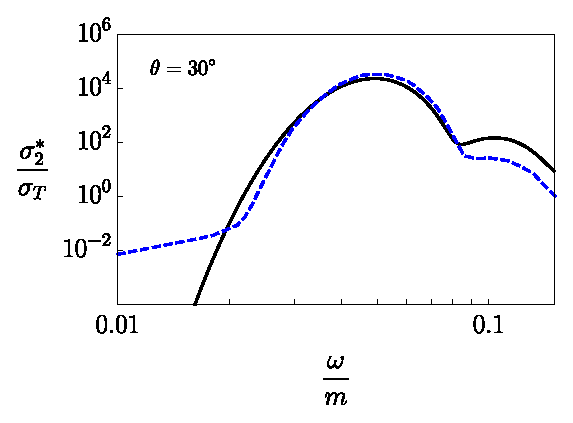
\includegraphics[width=0.5\linewidth,clip]{CompareMushOs005MushtukovO1Ground.eps}
	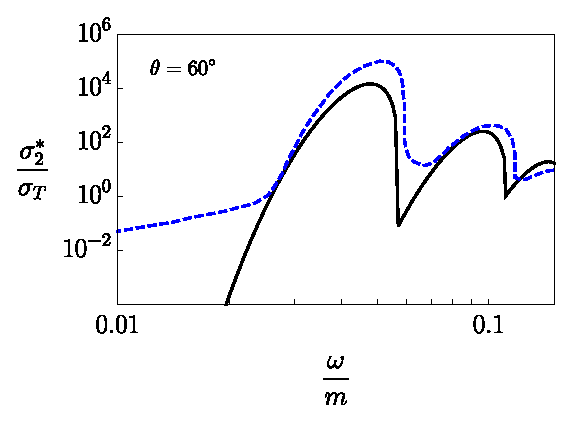
\includegraphics[width=0.5\linewidth,clip]{CompareMushOs005MushtukovO2Ground.eps}
	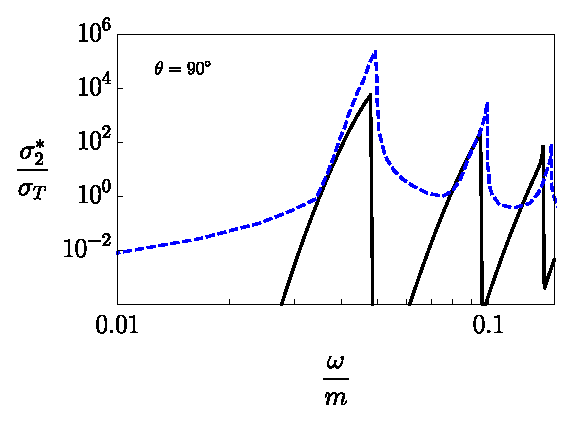
\includegraphics[width=0.5\linewidth,clip]{CompareMushOs005MushtukovO3Ground.eps}
	\caption{То же, что и на рис.~\ref{fig:CompAndMushXGround} для параметров плазмы $B=2.2\times 10^{12}$ Гс, $T = 20$ кэВ, $\mu=0$.}
	\label{fig:CompAndMushO}
\end{figure}
\clearpage



Рассмотрим теперь ситуацию сверхсильного магнитного поля, \linebreak\mbox{$B\sim 10^{15}-10^{16}$} Гс и высоких температур $T=1$ МэВ, которые характерны для гигантских вспышек SGR (источников мягких повторяющихся гамма-всплесков).  Исследование комптоновского процесса в магнитных полях указанного масштаба было проведено, например, в работе~\cite{Chistyakov:2009}. Однако, полученные в этом исследовании результаты будут справедливыми только для области энергий фотонов вдали от резонансов. Поэтому представляет самостоятельный интерес вычислить коэффициент поглощения фотона в пределе сильного поля с учетом возможного резонанса на виртуальном электроне с конечной шириной резонансного пика и сравнить с нерезонансным пределом~\cite{Chistyakov:2009} и дельта-функциональным приближением~\cite{Rumyantsev:2017}. Поскольку в пределе сильного магнитного поля начальный и конечный электроны будут преимущественно занимать основной уровень Ландау, а виртуальный электрон -- первый уровень Ландау, то коэффициент поглощения фотона с учетом конечной ширины резонансного пика примет достаточно простой для вычисления вид. Как было отмечено в разделе 1.3, в сильном магнитном поле энергии фотона, на которых наблюдается резонанс, выше, чем порог рождения $e^+e^-$ пары $q_{\mprl}^2=4m^2$ для фотона моды 2 , то целесообразно рассмотреть только каналы рассеяния $e\gamma^{(1)}\to e\gamma^{(1)}$ и $e\gamma^{(1)}\to e\gamma^{(2)}$. Следует отметить, что для фотона моды~1 порог рождения $e^+e^-$ пары $q_{\mprl}^2=(M_1+m)^2$ заведомо выше рассматриваемой области резонанса $q_{\mprl}^2=(M_1-m)^2$.

Исходя из результатов работы~\cite{Chistyakov:2009}, представим парциальные амплитуды комптоновского процесса в пределе сильного магнитного поля в виде:
\begin{equation}\begin{gathered}\label{amplnonres}
		{\cal M}_{e\gamma^{(1)}\to e\gamma^{(1)}}=\frac{8i\pi\alpha m}{\beta}\frac{(q\varphi q')(q\tilde{\varphi}q')}{\sqrt{q^2_\perp q^{'2}_\perp (-Q^2_{\mprl})}}\, ,\\
		{\cal M}_{e\gamma^{(1)}\to e\gamma^{(2)}}=\frac{8i \pi\alpha m}{\beta}\frac{(q\Lambda q')(q\tilde{\Lambda} Q)}{\sqrt{q^2_\perp {q'}^2_{\mprl}(-Q^2_{\mprl})}}\, ,\hspace{2mm} 
\end{gathered}\end{equation}
где   
$Q^2_{\mprl} = (q - q')^2_{\mprl} <0$,
$q_{\alpha} = (\omega,{\bf k})$ и $q'_{\alpha} = (\omega',{\bf k'})$
-- 4-импульсы начального и конечного фотонов соответственно.

После подстановки (\ref{amplnonres}) в
(\ref{eq:WabsStrongB}) коэффициенты поглощения фотона для каналов $e\gamma^{(1)}\to e\gamma^{(1)}$ и $e\gamma^{(1)}\to e\gamma^{(2)}$ в нерезонансной области для фотонов, распространяющихся под углом $\theta=90^\circ$ по отношению к направлению магнитного поля,  могут быть представлены следующим образом:
\begin{equation}\label{Wnonres}\begin{aligned}
		W_{e\gamma^{(1)}\to e\gamma^{(1)}}&=\frac{\omega \alpha^2m^2}{2 \beta \pi}\int dQ_0 dk_z' \frac{{k_z'}^2}{(-Q_{\mprl}^2)^2\varkappa}\theta(-Q_{\mprl}l^2)
		\theta({q'}_{\mprl}^2)\times\\&\times \sum_{\sigma} f(E_\sigma)(1-f(E_\sigma+\omega))(1+f_{\omega'})\, ,
\end{aligned}\end{equation}
\begin{equation}
	\begin{aligned}\label{Wnonres2}
		W_{e\gamma^{(1)}\to e\gamma^{(2)}}&=\frac{ \alpha^2m^2}{2 \beta \pi \omega}\int dQ_0 dk_z'\left(1-\frac{{\cal P}^{(2)}(q')}{{q'}_{\mprl}^2}\right) \frac{{q'}_{\mprl}^2-\omega\omega'}{(-Q_{\mprl}^2)^2\varkappa}\theta(-Q_{\mprl}^2)
		\theta({q'}_{\mprl}^2)\times\\ &\times\sum_{\sigma} f_{E_\sigma}(1-f_{E_\sigma+\omega})(1+f_{\omega'})\, ,
	\end{aligned}
\end{equation}
\noindent где $\theta(x)$ -- функция Хевисайда,
\mbox{$\varkappa = \sqrt{1 - 4m^2/Q^2_{\mprl}}$, $E_\sigma=\sqrt{p_{z\sigma}^2+m^2}$}, а \linebreak $p_{z\sigma}$ -- корни уравнения $Q_0+E_\sigma-E'_\sigma=0$:
\begin{equation}\label{savelaw}
	p_{z\sigma}=-\frac{Q_z}{2}+ \sigma Q_0 \varkappa\, .
\end{equation} 

Воспользовавшись результатами работы~\cite{Chistyakov:2009}, амплитуды ${\cal M}_{e\gamma^{(1)}\to e\gamma^{(1)}}$, ${\cal M}_{e\gamma^{(1)}\to e\gamma^{(2)}}$ в пределе сильного магнитного поля и с учетом конечной ширины резонансного пика можно представить следующим образом:
\begin{equation}\label{Mres}
	\begin{aligned}
		{\cal M}_{e\gamma^{(1)}\to e\gamma^{(1)}}=& \frac{8m\pi\alpha}{\sqrt{(-Q^2_{\mprl})}} \exp\left[-\frac{q^2_\perp+q'^2_\perp-2i(q\varphi q')}{4\beta}\right]\cdot\frac{1}{\sqrt{q^2_\perp q'^2_\perp}}\times 
		\\ &\times \sum_{n=1}^{\infty}\frac{((q\Lambda
			q')-i(q\varphi
			q'))^{n}}{(n-1)!(2\beta)^{n-1}}
		\frac{(q\tilde{\varphi}q')}{(p+q)^2_{\mprl}-M_n^2+iE''_n\Gamma_n }+\\
		&+(q\leftrightarrow-q')\, ,
	\end{aligned}
\end{equation}
\begin{equation}\label{Mres12}
	\begin{aligned}
		{\cal M}_{e\gamma^{(1)}\to e\gamma^{(2)}}=& \frac{8m\pi\alpha}{\sqrt{(-Q^2_{\mprl})}} \exp\left[-\frac{q^2_\perp+q'^2_\perp-2i(q\varphi q')}{4\beta}\right]\cdot\frac{1}{\sqrt{q^2_\perp q'^2_{\mprl}}}\times 
		\\ &\times \sum_{n=1}^{\infty}\frac{((q\Lambda
			q')-i(q\varphi
			q'))^{n}}{(n-1)!(2\beta)^{n-1}}
		\frac{(Q\tilde{\Lambda}q')}{(p+q)^2_{\mprl}-M_n^2+iE''_n\Gamma_n }+\\
		&+(q\leftrightarrow-q')\, ,
	\end{aligned}
\end{equation}
где полная ширина поглощения электрона $\Gamma_n$  является выражением~(\ref{eq:weldon}).С другой стороны, как показывает численный анализ, в случае сильно замагниченной, горячей, зарядово-симметричной плазмы полная ширина поглощения электрона мало отличается от соответствующего выражения в сильном магнитном поле и ультрарелятивистских электронов~\cite{KM_Book_2013}:
\begin{equation}\label{Shir}
	\begin{aligned}
		E''_n\Gamma_n=&\alpha \beta \sum_{n'=0}^{n-1}\int_{0}^{(\sqrt{n}-\sqrt{n'})^2}\frac{dx}{\sqrt{(n+n'-x)^2-4n n'}}\times\\
		&\times\{(n+n'-x)[{\cal I}^2_{n,n'-1}(x)+{\cal I}^2_{n-1,n'}(x)]-\\
		&-4\sqrt{nn'}{\cal I}_{n,n'}(x){\cal I}_{n-1,n'-1}(x)\}\, ,
	\end{aligned}
\end{equation}
где $E''_n=E+\omega$ -- энергия виртуального электрона.

 Парциальные коэффициенты поглощения фотона для каналов\linebreak $e \gamma^{(1)} \to e\gamma^{(1)}$ и $e \gamma^{(1)} \to e\gamma^{(2)}$ с учетом конечной ширины поглощения электрона могут быть получены подстановкой амплитуд~(\ref{Mres}) и~(\ref{Mres12}) в~(\ref{eq:WabsStrongB}) и в случае, когда начальный фотон распространяется поперек магнитного поля, коэффициенты поглощения можно представить следующим образом:


\begin{equation}\nonumber
	\begin{aligned}\label{Wres}
		&W_{e\gamma^{(1)}\to e\gamma^{(1)}}=\frac{\beta\alpha^2m^2}{\pi} \int dQ_0dk'_z \frac{{k_z'}^2\omega } {(-Q_{\mprl}^2)^2\varkappa}\exp\left[-\frac{\omega^2+{q'}_\perp^2}{2\beta}\right]\times\\ 
		&\times\sum_{n=1}^{\infty}\sum_{\sigma=\pm 1}\frac{1}{[(n-1)!]^2}\left(\frac{\omega \sqrt{q_\perp'^2}}{2\beta}\right)^{2(n-1)}\bigg\{
		\frac{1}{((p_\sigma+q)_{\mprl}^2-M_n^2)^2+(E''_n\Gamma_n)^2}  +\\
		&+\frac{1}{((p_\sigma-q')_{\mprl}^2-M_n^2)^2+(E''_n\Gamma_n)^2}-
		\\
		&-2
		\sum_{n'=1}^{\infty}\frac{(n-1)!}{(n'-1)!}\left(\frac{\omega \sqrt{q_\perp'^2}}{2\beta}\right)^{n'-n}J_{n+n'}\left(\frac{\omega \sqrt{q_\perp'^2}}{\beta}\right)\times\\
		&\times\frac{[(p_\sigma+q)^2_{\mprl}-M_n^2][(p_\sigma-q')^2_{\mprl}-M^2_{n'}]+E''_n\Gamma_nE''_{n'}\Gamma_{n'}}{[((p_\sigma-q')_{\mprl}^2-M_n^2)^2+(E''_n\Gamma_n)^2][((p_\sigma+q)_{\mprl}^2-M_{n'}^2)^2+(E''_n\Gamma_{n'})^2]}
		\bigg\}\times
		\\&\times f_{E_\sigma}(1-f_{E_\sigma+Q_0})(1+f_{\omega'}
		) \, ,
	\end{aligned}
\end{equation}

\begin{equation}
	\begin{aligned}\label{Wres2}
		&W_{e\gamma^{(1)}\to e\gamma^{(2)}}=\frac{\beta\alpha^2m^2}{\pi} \int dQ_0dk'_z \frac{q_\perp'^2\omega } {(-Q_{\mprl}^2)^2\varkappa}\exp\left[-\frac{q_\perp^2+{q'}_\perp^2}{2\beta}\right]\times\\ 
		&\times\sum_{n=1}^{\infty}\sum_{\sigma=\pm 1}\frac{1}{[(n-1)!]^2}\left(\frac{\omega \sqrt{q_\perp'^2}}{2\beta}\right)^{2(n-1)}\frac{Q_0}{\omega}\bigg\{
		{((p_\sigma+q)_{\mprl}^2-M_n^2)^2+(E''_n\Gamma_n)^2}+
		\\
		&+\frac{Q_0 \omega}{ q'^2_{\mprl}}\frac{1}{((p_\sigma-q')_{\mprl}^2-M_n^2)^2+(E''_n\Gamma_n)^2}-
		\\
		&-2
		\sum_{n'=1}^{\infty}\frac{(n-1)!}{(n'-1)!}\left(\frac{\omega \sqrt{q_\perp'^2}}{2\beta}\right)^{n'-n} J_{n+n'}\left(\frac{\omega \sqrt{q_\perp'^2}}{\beta}\right)\times\\
		&\times\frac{[(p_\sigma+q)^2_{\mprl}-M_n^2][(p_\sigma-q')^2_{\mprl}-M^2_{n'}]+E''_n\Gamma_nE''_{n'}\Gamma_{n'}}{[((p_\sigma-q')_{\mprl}^2-M_n^2)^2+(E''_n\Gamma_n)^2][((p_\sigma+q)_{\mprl}^2-M_{n'}^2)^2+(E''_n\Gamma_{n'})^2]}
		\times\\&\times
		\frac{Q_0(\omega-Q_0)}{q'^2_\perp}
		\bigg\}f_{E_\sigma}(1-f_{E_\sigma+Q_0})(1+f_{\omega'}
		) \, ,
	\end{aligned}
\end{equation}
\noindent где $J_n(x)$ -- функция Бесселя целого индекса, $p^\alpha_{\sigma\mprl}=(E_\sigma,p_{z\sigma})$. Поперечная составляющая импульса конечного фотона определяется из уравнения дисперсии:
\begin{equation}
	q'^2_{\mprl}=q'^{2}_\perp + {\cal P}^{(\lambda)}(q') .
\end{equation}

Имеет смысл провести сравнительный анализ результатов работы \cite{Chistyakov:2009}  с резонансным случаем (\ref{Wres}) и (\ref{Wres2}) для зарядово-симметричной плазмы и поперечного направления распространения импульса фотона по отношению к внешнему магнитному полю для различных значений величины магнитного поля, температуры и энергии начального фотона.



На рис.~\ref{Graph11B200T1}--\ref{Graph11B20T1} показан  коэффициент поглощения $W_{1\to1}$ рассеяния при температуре $T=1 $~МэВ и величине магнитного поля $B=200B_e$ и $B=20B_e$ соответственно. Как видно из рис.~\ref{Graph11B200T1}--\ref{Graph11B20T1}, коэффициент поглощения для канала $\gamma^{(1)}e\to\gamma^{(1)}e$ согласуется с соответствующими результатами для предела сильного поля и отсутствия резонанса, полученными в работе \cite{Chistyakov:2009} вплоть до энергий начального фотона  $\omega\simeq3$~МэВ для поля $B=200B_e$ и  $\omega\simeq0.3$~МэВ для поля $B=20B_e$. Отсюда вытекает ограничение на применимость результатов работы \cite{Chistyakov:2009} по энергиям начального фотона. Аналогичная ситуация наблюдается и для канала $\gamma^{(1)}e\to\gamma^{(2)}e$ (см. рис. \ref{Graph12B200T1}--\ref{Graph12B20T1}).  На рис. \ref{Graph11B20T1} и \ref{Graph12B20T1} наиболее ярко видно завышение коэффициента поглощения даже при относительно малых энергиях начального фотона. Этот факт связан с тем, что в пределе сильного магнитного поля разложение амплитуды комптоновского процесса по обратным степеням поля уже не будет правомочным.  

Следует отметить   что при относительно малых температурах $T\lesssim50$ кэВ с тем же магнитным полем $\delta$-аппроксимация работает хуже из-за уменьшения области резонанса. В целом $\delta$-функциональное приближение достаточно хорошо описывать лишь первый резонансный пик.

Следует отметить   что при относительно малых температурах $T\lesssim50$ кэВ с тем же магнитным полем $\delta$-аппроксимация работает хуже из-за уменьшения области резонанса. В целом $\delta$-функциональное приближение достаточно хорошо описывать лишь первый резонансный пик.
\clearpage
\begin{figure}[t!]\centering
	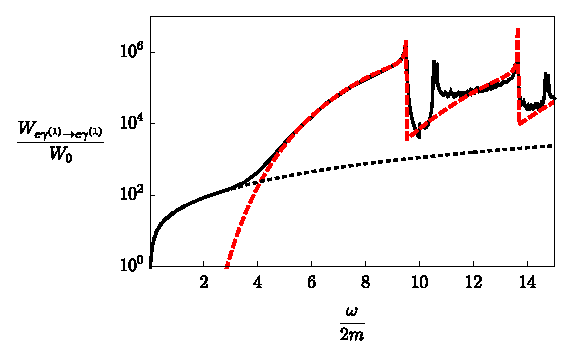
\includegraphics[width=0.8\linewidth]{Splot112001.eps}
	\caption{Зависимость коэффициента поглощения от энергии начального фотона для канала $e\gamma^{(1)}\to e\gamma^{(1)}$ при поле $B=200 B_e$ и температуре T=1 МэВ: сплошная линия -- коэффициент поглощения с учетом резонанса; штриховая линия -- без учета резонанса; пунктирная линия -- дельта-функциональное приближение. Здесь $W_0=(\alpha/\pi)^3m\simeq 3.25\cdot10^2$ см$^{-1}$.}
	\label{Graph11B200T1}
\end{figure}

\begin{figure}[t!]\centering
	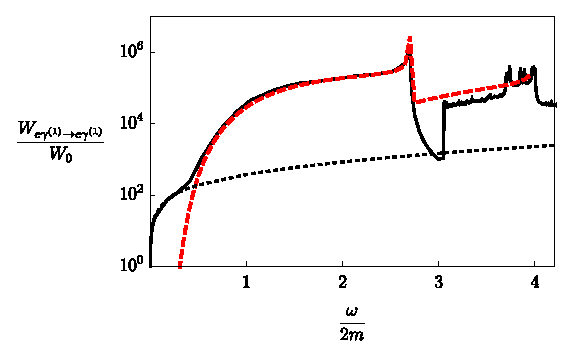
\includegraphics[width=0.8\linewidth]{Splot11201.eps}
	\caption{Зависимость коэффициента поглощения от энергии начального фотона для канала $e\gamma^{(1)}\to e\gamma^{(1)}$ при поле $B=20 B_e$ и температуре T=1 МэВ. Обозначение для линий то же, что и для рис. \ref{Graph11B200T1}.}
	\label{Graph11B20T1}
\end{figure}

\begin{figure}[t!]\centering
	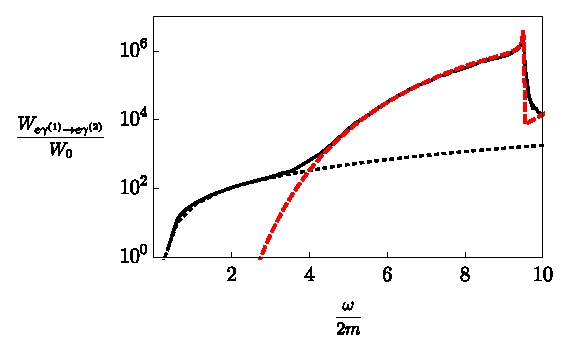
\includegraphics[width=0.8\linewidth]{Splot122001.eps}
	\caption{Зависимость коэффициента поглощения от энергии начального фотона для канала $e\gamma^{(1)}\to e\gamma^{(2)}$ при поле $B=200 B_e$ и температуре T=1 МэВ. Обозначение для линий то же, что и для рис. \ref{Graph11B200T1}.}
	\label{Graph12B200T1}
\end{figure}

\begin{figure}[t!]\centering
	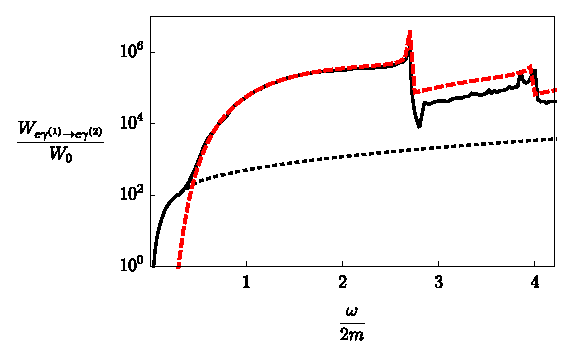
\includegraphics[width=0.8\linewidth]{Splot12201.eps}
	\caption{Зависимость коэффициента поглощения от энергии начального фотона для канала $e\gamma^{(1)}\to e\gamma^{(2)}$ при поле $B=20 B_e$ и температуре T=1 МэВ. Обозначение для линий то же, что и для рис. \ref{Graph11B200T1}.}
	\label{Graph12B20T1}
\end{figure}
\clearpage
\label{Ch:Compton}
������� � �������� �������������� ��������� $\gamma e \to \gamma e$ � 
������� ��������� ���� ������������� ��� ������ ����������� ��������� ������������ 
������������ ����� � ������� ������������� 
���������~\cite{Truemper1978,Makishima1990,Grove1995}, ������� ���������� 
������������������ ���� ��� ������������ ����������, ���� ��� ������������ 
���������~\cite{Truemper1978}. ���������� ��������� ���������� ���������� �� 
������� ��������� �������� ���������, ��� ������������ ����������� ������� 
������ � ����������� ����������� ������~\cite{Mihara:1990}.
��� ���� ��� ������������ ���������� ������ ���������� 
������ ���������� ������� ��������� �� ��������� � ������������ ������������ 
�������� $\sigma_T = 8 \pi \alpha^2 /(3 m^2)$. � ����� �� ������ 
����� �� ���� ��������~\cite{Canuto:1971} ��������� ��� ������� 
�������������� 
��������� � ��������� ���� ��� ������ ���� ��������
� ���������������� ������� � ��� ������, 
������������������� ����� ���������� ����, � ������� ��� ��������� ����������� 
��� ��� �������:
\begin{equation}\label{eq:w_B}
	\omega_B\simeq \frac{\beta}{m}.
\end{equation}
 
����� ����, � ������~\cite{Canuto:1971} ����� ���� ��������, ��� ������� ��������� ������ 
�� ���������
����������� ������� ��� �� ���������������� ��������� ������, ��� � �� ���� 
����� ������������ �������� ���������� ������ � ������������ ���������� ����. � 
������������� �� ��� 
������~\cite{Gnedin1973} 
������������� ��������� ������� ������ � ������������� ��������, ������� 
������������ ������� $\omega_B$~(\ref{eq:w_B}). 
� ��������� �������~\cite{Borner1979,Ventura:1979} 
���� �������� ���������� ��� ������� ������� ��������� ������ �� ��������� � �������������� ���������� ������~\cite{Canuto:1971}, ������� ����� ������������� ������ ��� ������������ ������� ���������� ����~$B<10^{12}$~��. ������ ��� ��������� ���������� ����~$B>10^{12}$~��, ��� ���� �������� � �������~\cite{Herold:1979,Melrose:1983III},   ���� �������������� �������� � ������� �������������� ��������� ���������� 
������������.


% B/B_e=1 � B/B_e=0.1
� �������������� ���� ������� ��������������, ��� ��������� � �������� ��������� ��������� 
�� �������� ������ ������, ��� ����� ����� � ������� �������� ���������� ���� 
�/��� ������ ���������� $T\ll m$ (��. ��������). � ���� ������� ����������� 
���~(\ref{eq:w_B})  ��������� � ������� ����� ������ ������� ������, � ����� 
���� ��������� ����������� ��� ����������� �����, ��������������� ������ 
������� ������ $n$ 
������������ ���������. ��� ���� ����������� ��� �������� ������:
\begin{equation}\label{eq:whn}
	\omega_n(\theta)= \frac{\sqrt{m^2+2 \beta n \sin^2\theta} - 
		m}{\sin^2\theta}\, ,
\end{equation}
��� $\theta$ -- ���� ����� ��������� ���������� ������ � ������������ 
���������� ����. 

� ������ �������, � ���������� �������������� �������� ����� ������������ 
������ ������ ������ ���������� ���������, ���, � ���� �������, ����� ��������� 
���������� �������� ������� ����� ������� ��� ��������� ����� $B\lesssim 
B_e$~\cite{Daugherty:1986,Bussard:1986}. � ����� ������ ��� ������������ ������� ������ $\ell$ ���������� ��������� ����������� 
���� ����� ����������� �� ��������:
\begin{equation}\label{eq:resAll}
	\omega_{n\ell}(\theta)=\frac{\sqrt{M_\ell - \sin^2\theta (M_\ell^2-M_n^2)}-M_\ell}{\sin^2\theta}\, ,
\end{equation}
��� $M_\ell=\sqrt{m^2+2\beta \ell}$, $M_n=\sqrt{m^2+2\beta n}$ � �.�.



%������� �������������� �������� � ���������������� ������� � ������������� ������ ��������������� � ������~\cite{Canuto:1971}. ������ ��� ��������� ���������� ���� $B>10^{12}$ �� ���� �������������� �������� ���������� ������������, ��� ���� �������� � ���� �����~\cite{Bulik:1997,Chistyakov:2009,Gonthier:2014,Mushtukov:2016}.

% ���-�� ����� ������� � ������
� ������������� ���� ������� ������� �������������� ��������� 
���������� ����������� ��� �������� ������, ��������������� ������������ 
����������~(\ref{eq:whn}) ���������� ������������� � 
������� ������� ����� ����������� ������. �� ���� ������� �� ���������� 
����������� ������ ��� �������� ������� ������ ����� �� ����������
� ����� ���� ���������, ��������, ��� ������������� ��������� 
	\textcolor{red}{������������� 
	�������� ������ ������ ����������� ���������� 
	�����~\cite{Ozel:2001} ��� �� ��� ������������ ������ ���������\linebreak ����� $B\lesssim 10^{10}$ ��~\cite{Zavlin:1996}.}

� ������ �������, ���� ���������� � ������������� �������� �������� ����������� 
��� ������������� �������� ��������� ������ ������������� ���������� 
�����~\cite{Alexander:1991,Araya:1999,Ho:2001,Lyutikov:2006,Potekhin:2004,Schonherr:2007,Nishimura:2008,Suleimanov:2009}.
������ ����������� ���������� ������, ��� ����������� ���������, ����������� 
�������� ������������� ������� ��������� ������� ����� ������� �� �������������������� ���������� 
�������� ������������ ���������, ������� �������� � ���������� ������ 
���������� ������������ � ����������� ��������������������� ������ � ������� 
���������~\cite{Fernandez:2007,Nobili:2008,Baring:2018,Beloborodov:2013}.
%Ozel2001: ������� ��������� ������ ������������ ��������� �� � ��������������� ������������ ����������� ������ ��� �������. ��������� ��������� ������������ � ��������� ����� � ��������� ����������������� ����������. ��������� ������. 10^13<B<10^15. ������ �������� ������.
%Zavlin:1996 ������ ���� ��� ������� ����������� �������.
%

������ 
������������ ���������� ��� ������� ������� 
�������������� ��������� ��������� ������ ������ 
������ ��������� ��������� \linebreak ���������~(��. ���������� \ref{appA:AccurProp}). � ���������������� 
�������~\cite{Canuto:1971} ������������ ���� ���� ����������� 
�������~(\ref{eq:whn}) � ������� ���������
�� ������� �� ���������������� ��������� ��������� (��� ��� ��������� ���������), 
������� ������ ������ ������ ������������ ������~\cite{Daugherty:1989}. ������ 
� ������� ��������� �����~$B\gtrsim B_e$ � ��� ������� �������� ������ 
��������� ��������� �������������� ��������, ��� �������� � ����, ��� ��������� 
���  ������� 
���������� ����� ����������, ��������� ��� ����� ����������� ����� 
����������~(\ref{eq:resAll}), 
������������ � ����� �� ���� ������������� ����������� ����������.

���������� ��� ����� �������� ����������� ����� �������������� ����������� �� ����� ������ ������� �������������� ���������~\cite{Gonthier:2000}. 
��� ���� ������� � ������~\cite{Gonthier:2014}, ����� ������ �� �������� 
������, ��������� ���������� �� ����� ����������� ��������� �������� 
����������� ������� ������� ������������ ���������, ��� �������� � ��������� �������� ������� �������������� ��������� � ����� 
���������. ���� ���������� ��� �������� � ������~\cite{Mushtukov:2016}, ��� 
������������ ������� ��������� �������� $\gamma e\to \gamma e$ � ������ 
������ ������� ����������� ������������� ���������, ������� 
������� �� 
���������������� ��������� ���������. 
������ ������ ������� �������������� ���������, ���������� ����� �������, 
������������ ����� ���������� ���������, ���, ��������, ���������� ��� 
������������� � ������� �������� ���������. 

� ���� ������� ��������� ������� ��������� ����� ��������� ��� ��������� 
�������������� 
������� ��������� �����. 
���, � ������~\cite{Gonthier:2000} ���� ������������ 
������������� ������� ��������� � ������ ��������� � �������������������� 
������� ��� ������ ������������ �������� ���������� ���� $B>0.1 B_e$. � ����� 
������������� ��������� ����������� �������� ���������� �������� � ����������� 
�� �������� �������������� �������, ������� �����������
�������������� ��������� �������� � ����������� �������������� �������� 
���������� ������ ���������� $\gamma 
e \to e$. � 
������~\cite{Harding:1991} ������������ ������ ������������� �������������� 
������� � ������� �������������� �������� ���������� ������ ���������� ��� 
��������� ����� 
$B\sim 
0.1B_e$. �������� ����� ������������� ��������� ���������� � ������������� 
���������� ���������� ������������ �� ������ ������������ ���������� ��-�� 
�������������� ������. ��� ���� ������ ���������� � 
������~\cite{Rumyantsev:2017}, �� ����������� � ���, ��� ���������� 
������������ ��������� ����� �������� 
�� ������-�������, ����� �������� ����� 
� ������� ��������� ����� ������ ������� ������ ���������� (����������� ������ 
����). 
 
����� ���������� 
��������� ������� ��������� �������������� �������� � ������ ������ 
������������ ����.
��� ������� ������ ���������� ������������ ���������� ������ ���������� ����������� ����������, ����������� �������� ����� �������������� �������� $f$ � ����������� ������~$j$~\cite{KuzRumShlen:2015}:
\begin{equation}
	{\cal L}(x) \, = \, \sum \limits_{k} g_k 
	[\bar {\psi_f}(x) \Gamma_k \psi_f(x)] J_k(x), 
	\label{eq:L}
\end{equation}
��� $\psi_f(x)$ --  
��������� ����������� ����, � ������ $k = S, P, V, A$ ������������� ���������, ���������������, ��������� � ���������� �������� � ��������� $\Gamma_k$:    
%\newline
$\Gamma_S = 1, \, \Gamma_P = \gamma_5, \, \Gamma_V = \gamma_{\alpha},
\, \Gamma_A = \gamma_{\alpha} \gamma_5$, ��������������� ���������� ���������� �����
$J_k(x)$ ($J_S$, $J_P$, $J_{V\alpha}$ ��� $J_{A\alpha}$), � ����� ���������� ��������������
$g_k$.

� ���������, ���������� ����������������� �������������� ����� ���� ����������� � ����:
%
\begin{eqnarray}\label{eq:L}
	{\cal L}(X) \, = \,- e [\bar \psi_f (X) \gamma^{\mu} A^{(\lambda)}_\mu (X) \psi_f(X)] \, ; 
	\label{eq:Lel}
\end{eqnarray}

\begin{figure}
	\centerline{
		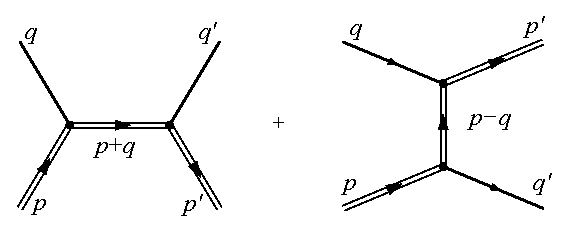
\includegraphics[width=10cm]{figComp1.eps}}
	\caption{��������� �������� ��� ������� $\gamma e \to \gamma^{\, \prime} e^{\, \prime}$. 
		������� ����� ��������, ��� ������� �������� ���� �� ��������� � �������� ��������� ��������� 
		� �� ���������� ����������  ������ �����.}
	\label{fig:Diagjj}
\end{figure}
%

������������� ������� � ��������� ����������� ����������� ����������� ��������, ��������������� �� ���.~\ref{fig:Diagjj}. ��������������� $S$-��������� ������� ��������� ������ ����������� $\lambda$ �� ��������� � ��������� ��������� � ������ ����������� $\lambda'$, � ������ �����������~(\ref{eq:L}) ����� ���� ����������� � ����:  
%
\beq                          
\nonumber
S^{s^{\, \prime} s}_{\gamma^{(\lambda)} e \to \gamma^{(\lambda')} e'} &=& - e^2\int \dd^4 X \dd^4 Y A^{(\lambda)}_\mu (X) A^{(\lambda')}_{\mu'} (Y)
%\times 
%\\[3mm]
%\nonumber
%&\times& 
\, \left [\bar \Psi^{s'}_{p',\ell'}(Y) \gamma_{\mu'} 
S(Y,X) 
\gamma_\mu \Psi^{s}_{p,\ell}(X) \right ]\, +
\\[3mm]
\label{eq:S1a}
&+& (A^{(\lambda)}_\mu, \gamma_\mu \leftrightarrow A^{(\lambda')}_{\mu'}, \gamma_{\mu'})\, .
\eeq

\noindent ����� $p^{\mu} = (E_{\ell}, {\bf p})$ � $p^{\, \prime \mu} =
(E^{\, \prime}_{\ell'}, {\bf p}^{\, \prime})$ - ������������� ������� 
�������-�������� ���������� � ��������� ���������, ����������� �� ������� ������ 
$\ell$ � $\ell'$  ��������������,
$\Psi^s_{p,\ell}(X)$ - �������� ������� ���������� � ����������� �������� 
���������� ����~(\ref{eq:psie}), $s$ � $s'$ ���������� 
��������������� ��������� ���������� � ��������� ��������� 
��������������, $S(Y,X)$ -- ���������� ��������� �� ������� ��������� ����~(��. ����������~(\ref{eq:propagator}). 

�������� ������� ������ $A^{(\lambda)}_\mu(X)$ � $A^{(\lambda')}_{\mu'}(Y)$, � ���� �������,  ������ ����������� � ���� �������������� ������� � ����������� $\varepsilon^{(\lambda)}_\mu(q)$ � $\varepsilon^{(\lambda')}_{\mu'}(q')$:
%
\begin{eqnarray}
	\label{eq:j_k}
	A^{(\lambda)}_\mu (X) = \frac{e^{-\ii(qX)}}{\sqrt{2q_0 V}} \, \varepsilon^{(\lambda)}_\mu(q) \, , \quad  q^{\alpha} = (q_0, {\bs q})\, ,
\end{eqnarray}
%
\begin{eqnarray}
	\label{eq:j_k'}
	A^{(\lambda')}_{\mu'} (Y) = \frac{e^{\ii(q'Y)}}{\sqrt{2q'_0 V}} \, \varepsilon^{(\lambda')}_{\mu'}(q') \, , \quad  q'^{\alpha} = (q'_0, {\bs q'})\, , 
\end{eqnarray}
\noindent ���  $V = L_x L_y L_z$ -- ������������� �����.

� ������ ���� ���������, ��������� �������~(\ref{eq:psie}),  �����-������ �������� ������� �������~(\ref{eq:j_k}),
����������~(\ref{eq:propagator})  �~(\ref{eq:S1a}).  ��������������� ���������� ��������� �� $\dd X_0 \dd X_2 \dd X_3$ �  $\dd Y_0 \dd Y_2 \dd Y_3$,  ����������  $S$-��������� �������  � ��������� ����:
%
\begin{eqnarray}
	%\nonumber
	\label{eq:S2}                                  
	{\cal S}^{s^{\,\prime} s}_{\gamma^{(\lambda)} e\to \gamma^{(\lambda')} e} = \frac{\ii (2\pi)^3 
		\delta^{(3)}_{0,y,z} (P - p^{\, \prime} - q^{\, \prime})}
	{\sqrt{2q_0 V 2q^{\, \prime}_0 V 2 E_{\ell} L_y L_z 2 E^{\, \prime}_{\ell'}L_y L_z}}\, 
	{\cal M}^{s^{\, \prime} s}_{\gamma^{(\lambda)} e\to \gamma^{(\lambda')} e'} \, , 
\end{eqnarray}
\noindent ��� $\delta^{(3)}_{0,y,z} (P - p^{\, \prime} - q^{\, \prime}) 
= \delta (P_0 - E^{\, \prime}_{\ell'}-q^{\, \prime}_0) 
\delta (P_y - p^{\, \prime}_y - q^{\, \prime}_y) 
\delta (P_z - p^{\, \prime}_z - q^{\, \prime}_z)$, 

\begin{eqnarray}
	\label{eq:M12a}                                  
	%\nonumber
	&&{\cal M}^{s^{\, \prime} s}_{\gamma^{(\lambda)} e_\ell\to \gamma^{(\lambda')} e_{\ell'}} \simeq \ii e^2 \varepsilon^{(\lambda')}_{\, \mu'}(q') \varepsilon^{(\lambda)}_{\mu}(q) 
	%\times 
	%\\
	%\nonumber  
	%&&\times 
	\, \sum\limits_{n=0}^{\infty} \sum\limits_{s''} \; 
	\int \dd X_1 \dd Y_1 \eee^{-\ii X_1 q_x + \ii Y_1 q'_x}  \times
	\\ [3mm]
	\nonumber  
	&&\times \frac{\bar \phi^{s'}_{p', \ell'} (Y_1) \gamma_{\mu'} \phi^{s''}_{P, n} (Y_1) 
		\bar \phi^{s''}_{P, n} (X_1) \gamma_{\mu}  \phi^{s}_{p, \ell} (X_1)}
	{P^{2}_{\mprl} - M_n^2 + \ii P_0 \Gamma^{s''}_n/2} + 
	\\ [3mm]
	\nonumber  
	&&+ (\varepsilon^{(\lambda)}_\mu (q), \gamma_\mu, P, q \leftrightarrow \varepsilon^{(\lambda')}_{\mu'}(q'), \gamma_{\mu'}, P', -q')\, ,
\end{eqnarray}
\noindent  $P_\alpha = (p+q)_\alpha$, $P'_{\alpha} = (p-q')_{\alpha}, \,\, \alpha =0,2,3$.

�������, ��� ����� �������� ���������~(\ref{eq:M12a}) ����� ����� ����������� ��������. ���� ����������� ������� $\ell,\ell'\geqslant n$, �� � ���� ������ � ����������� �������� ���������� �����, ��������������� ����, ��� ����������� ������� ���������� ��������, �� ���� ����������� ��������� $P^{2}_{\mprl} - M_n^2 = 0$. ��� ������� $\ell,\ell'<n$ ������, ���������� �� ��������� � �����������, ����������� � �������� �� ����������� �������� �� �����������. ����� ����, �������������� ������ ����������, ��� ������ ������ ������������ ���������� �������� ����� � ��������� �������������� �������� $\gamma e\to \gamma e$ ����� ������ ������ ������ (�.�. s-���������) ���������.

\textcolor{red}{��������~\cite{Weldon:1983}, ������ ������ ��������� ��������� ��������� $\Gamma_n^{s''}$ ����� ����������� �
	���� ����� ����� ����������, $\Gamma^{(abs)\, s''}_n$, � ��������, $\Gamma^{(cr) \, s''}_n$,  ��������� 
	��������� �������:}
\beq
\label{eq:weldon}
\Gamma_n^{s''} = \Gamma^{(abs)\, s''}_n + \Gamma^{(cr) \, s''}_n \simeq 
\Gamma^{(abs) \, s''}_{e_n \to e_{\ell'} \gamma} 
\left [1+ \eee^{-(E^{\, \prime \prime}_n - \mu)/T} \right ]\, ,
\eeq
\noindent ���
%
\beq
\label{eq:e_abs}
\Gamma^{(abs) \, s''}_{e_n \to e_{\ell'} \gamma}  &=& \sum\limits_{\ell' = 0}^{n-1} \;  \sum\limits_{s' = \pm 1} \; \sum\limits_{\lambda'} \; 
\int \frac{\dd p'_y \dd p'_z  L_y L_z }{(2\pi)^2} \,[1 - f_{-}(E^{\, \prime}_{\ell'})] \times 
\\
\nonumber
&\times& \frac{\dd^3 q' V}{(2\pi)^3} \, (1 + f_{\omega'}) \;
\frac{|{\cal S}^{s^{\,\prime} s''}_{e_n \to e_{\ell'} \gamma^{(\lambda')}}|^2}{\tau}  
\eeq 
\noindent -- ������ ���������� ��������� � �������� $e_n \to e_{\ell'} \gamma$.

��� ���� �������� � ������~\cite{RumShlenYar:2017}, � ������, ����� ������ ���������� ��������� $\Gamma_n$ ���������� ����, �� ��������� �������������� �������� ������������� ����� �������������� ����������. ���� ���� ��� ����������� ����������� ��������� ���������� �������, ��� ��������, ��������, � ����������� ���������� �������������� ������� ��������� ��������. ������ ������ ���� ����� ����. �������������, � ������� ���������, ��� ����������� ������� $P_0\Gamma^{s''}_n\ll \left|P^2\mprl-M_n^2\right|$ ��������������� ����� �~(\ref{eq:M12a}) ����� ���� �������� $\delta$-��������:
\begin{equation}\nonumber
	\left|\frac{1}{P^2_{\mprl}-M_n^2-\ii P_0\Gamma^{s''}_n/2}\right|^2
	\simeq\frac{2\pi}{P_0\Gamma_n^{s''}} \delta(P^2_{\mprl}-M_n^2).
\end{equation}

� ����� ������ ������� ����������� ��������� ����� ��������� ��������� �������
\beq
\label{eq:delta_f}\nonumber
&&|{\cal M}^{s^{\, \prime} s}_{\gamma^{(\lambda)} e_\ell \to \gamma^{(\lambda')} e_{\ell'}}|^2 \simeq  \sum\limits_{s'' = \pm 1} \sum\limits_{n=0}^{\infty} \;  
\frac{\pi}{P_0 \; \Gamma_n^{s''}} \; \delta (P^{2}_{\mprl} - M_n^2) \times 
\\  
&&\times \left | 
\int \dd X_1 \dd Y_1 \bar \phi^{s'}_{p'\ell'} (Y_1) \phi^{s''}_{P, n} (Y_1) \bar \phi^{s''}_{P, n} (X_1) \phi^{s}_{p \ell} (X_1) \right |^2  \, .
\eeq

� ������~(\ref{eq:delta_f}) ������� $S$-���������� �������� �������� 
$jf \to j^{\, \prime} f^{\, \prime}$ ������������� ����� �������������� �������������
%
\beq
\label{eq:S2factor}
\nonumber 
&&\sum\limits_{s, s' = \pm 1} \frac{|{\cal S}^{s^{\,\prime} s}_{\gamma^{(\lambda)} e_\ell \to \gamma^{(\lambda')} e_{\ell'}}|^2}{\tau} = 
\sum\limits_{s, s', s'' = \pm 1} 
\sum\limits_{n=0}^{\infty} \; \frac{(2\pi)^3 \delta^{(3)}_{0,y,z} (P - p^{\, \prime} - q^{\, \prime})}
{2q_0 L_x 2q^{\, \prime}_0 V 2 E_{\ell} L_y L_z 2 E^{\, \prime}_{\ell'}L_y L_z} \times
\\[3mm] 
&&\times 
\int \frac{\dd p^{\, \prime \prime}_y \dd p^{\, \prime \prime}_z}{(2 E''_n)^2 (2 \pi)^2 \; \Gamma_n^{s''}} \, 
(2\pi)^3 \, \delta^{(3)}_{0,y,z} (P - p'') 
|{\cal M}^{s^{\, \prime} s''}_{e_n\to \gamma^{(\lambda')} e_{\ell'}}|^2 \; |{\cal M}^{s'' s}_{\gamma^{(\lambda)} e_\ell \to e_n}|^2   \, .
\eeq

����� �� ��������������� ��������� $\delta$ - �������:
%
\begin{eqnarray}
	\label{eq:delta_prop}
	\delta (P^2_{\mprl} - M^2_n) = \frac{1}{2 E''_n} \, \delta (P_0 - E''_n) \, , 
\end{eqnarray}
%
\noindent ��� $E''_n = \sqrt{p^{\, \prime \prime 2}_z + M^2_n}$. 


���� ������ ������   $S$-��������� ������� ���������� ��������� ��������� �������
\beq
%\nonumber
\label{eq:Sjf}                                  
{\cal S}^{s^{\,\prime \prime} s}_{\gamma^{(\lambda)} e_\ell \to e_n} = 
\frac{\ii (2\pi)^3 
	\delta^{(3)}_{0,y,z} (P - p^{\, \prime \prime})}
{\sqrt{2q_0 V 2 E_{\ell} L_y L_z 2 E^{''}_{n} L_y L_z}}\, 
{\cal M}^{s'' s}_{\gamma^{(\lambda)} e_\ell \to e_n} \, ,
\eeq
� ������ ����, ���
\begin{equation}
	\left|\delta^{(3)}_{0,y,z}(P-p'')\right|^2=\frac{1}{(2\pi)^2}\delta_{0,y,z}^{(3)}(P-p'')\tau L_y L_z \, ,
\end{equation}
�������� ������, ��� ���������~(\ref{eq:S2factor}) 
����� ����������� � �������������� ����:
%
\beq
\label{eq:S2factor1}
\sum\limits_{s, s' = \pm 1} \frac{|{\cal S}^{s^{\,\prime} s}_{{\gamma^{(\lambda)} e_\ell \to \gamma^{(\lambda')} e_{\ell'}}}|^2}{\tau} = 
\sum\limits_{s, s', s'' = \pm 1} 
\sum\limits_{n=0}^{\infty} \;  \int \frac{\dd p^{\, \prime \prime}_y 
	\dd p^{\, \prime \prime}_z}{(2 \pi)^2 \; \Gamma_n^{s''}} \,  
\frac{|{\cal S}^{s^{\,\prime \prime} s}_{\gamma^{(\lambda)} e_\ell \to e_n}|^2}{\tau} \, 
\frac{|{\cal S}^{s^{\,\prime} s''}_{ e_n \to \gamma^{(\lambda')} e_{\ell'}}|^2}{\tau} \, .
\eeq
\noindent ����� ��������������� ��������� ${\cal M}^{s'' s}_{\gamma^{(\lambda)} e_\ell \to e_n}$ �������������� �������� ������������ ��������� �������:
%
\beq
\label{eq:amplonever} 
{\cal M}^{s'' s}_{\gamma^{(\lambda)} e_\ell \to e_n} =  \frac{\exp{[-\ii q_x (p_y + p_y^{\,\prime \prime})/(2\beta)]}}{\sqrt{M_{\ell} M_n (M_{\ell} + m) 
		(M_n + m)}} 
\left [ \frac{q_y+\ii q_x}{\sqrt{q_{\mprp}^2}} \right ]^{n-\ell} {\cal T}^{s'' s}_{V} \, ,
\eeq

$S$-��������� ������� ��� �������� �������� ������ $\gamma \to e\gamma$ ����� ���� ������� �� ���������� �������� �������� ���������� ������ ��������� ������� 
$S_{e_n \to \gamma^{(\lambda')} e_{\ell'}}=S_{\gamma^{(\lambda)} e_\ell \to e_n}(q\to q', E_\ell \to E'_{\ell'})$.

\textcolor{red}{�� �������� �� � ����������?} ����� �������, ��� ��������� ��������� �������������� �������� ������ ��������� � ������ ������ ����, ���������� ��������� ��������
${\cal T}^{s'' s}_{V}$, ������� ���� ������������ � ������~\cite{RumShlenYar:2017} ��� ������ ����������, ����������������, ���������� � ���������-���������� �����. ��� ���������� �����  
������-���������� � ����������~  � ���������������~$\{0, 3\}$:

\begin{equation}
	\label{eq:K1}
	{\cal K}_{1\alpha} = \sqrt{\frac{2}{(p\widetilde \Lambda p^{\, \prime \prime}) + 
			M_\ell M_{n}}} \left \{M_\ell (\widetilde \Lambda p^{\, \prime \prime})_\alpha + 
	M_{n} (\widetilde \Lambda p)_\alpha  \right \}\, ,
\end{equation}
%
\begin{equation}
	{\cal K}_{2\alpha} = \sqrt{\frac{2}{(p\widetilde \Lambda p^{\, \prime \prime}) + 
			M_\ell M_{n}}} \left \{M_\ell (\widetilde \varphi p^{\, \prime \prime})_\alpha + 
	M_{n} (\widetilde \varphi p)_\alpha  \right \}\, ,
	\label{eq:K2}
\end{equation}

\begin{equation}
	\label{eq:K3}
	{\cal K}_{3} = \sqrt{2\left [(p\widetilde \Lambda p^{\, \prime \prime}) + 
		M_\ell M_{n} \right]} \, ,  
\end{equation}
%
\begin{equation}
	\label{eq:K4}
	{\cal K}_4 = 
	- \sqrt{\frac{2}{(p\widetilde \Lambda p^{\, \prime \prime}) + M_\ell M_{n}}}\, 
	(p\widetilde \varphi p^{\, \prime \prime}) \, .
\end{equation}

��� ����������� ���� ������������ �����������:
%
\begin{equation}
	\label{eq:Ilnnl}
	\begin{aligned}
		\frac{1}{\sqrt{\pi}}\int \dd Z& \, \eee^{-Z^2}  
		H_n \!\! \left (Z + \frac{q_y + \ii q_x}{2\sqrt{\beta}} \right )   
		H_{\ell} \!\! \left (Z - \frac{q_y - \ii q_x}{2\sqrt{\beta}} \right ) =
		\\
		\nonumber
		&= 2^{(n+\ell)/2} \sqrt{n ! \, \ell !} 
		\left [\frac{q_y + \ii q_x}{\sqrt{q^2_{\mprp}}} \right ]^{n-\ell} 
		\eee^{{q^2_{\mprp}}/{(4\beta)}} 
		{\cal I}_{n, \ell} \!\! \left (\frac{q^{2}_{\mprp}}{2 \beta} \right ) \, , 
	\end{aligned}
\end{equation}
\noindent ��� ��� $n \geqslant \ell$
%
\begin{eqnarray}
	\nonumber
	&&{\cal I}_{n, \ell} (x) = \sqrt{\frac{\ell !}{n !}} \; \eee^{-x/2} x^{(n-\ell)/2} L_\ell^{n-\ell} (x) \, ,
	\\
	&&{\cal I}_{\ell, n} (x) = (-1)^{n-\ell} {\cal I}_{n, \ell} (x) \, ,
	\label{eq:Inl}
\end{eqnarray}
\noindent � $L^k_n (x)$ -- ���������� �������� �������~\cite{Gradshtein}.
����� � ������ ����� ������������ ����������� ${\cal I}_{n, \ell}\equiv{\cal I}_{n, \ell} \left(\frac{q_\perp^2}{2\beta}\right)$ � ��� �������������� ��������������� ���������, ��� ������� ���� ������ $\eta=-1$.

��� ��������������� ���������� ���������� ����������� ������ ������ ������� ������������ ����������� ���������� ������ -- ����������� �������� ������ � ������ ��������� �� ���� ��� ��� ���� ���������, ������� ��� �������������� �������� ��� ���������, ��������, � ������~\cite{Chistyakov:2009}:
\begin{eqnarray}\label{eq:WabsStrongB}
	&&W_{\gamma^{(\lambda)} e \to \gamma^{(\lambda')} e} = \frac{\beta}{16 (2\pi)^4
		\omega_{\lambda}}
	\int \mid {{\cal M}^{s'' s}_{\gamma^{(\lambda)} e_\ell \to \gamma^{(\lambda')} e_{\ell'}}}\mid^2 \times
	\label{eq:Wscatt}\\
	&&\times f_{E}\, [1-f_{E'}] \, (1 + f_{\omega'})
	\delta (\omega_{\lambda}({\bf k}) + E - \omega_{\lambda^{'}}({\bf k'}) - E')
	\frac{dp_z\,d^3 k^{'}}{ E E' \omega_{\lambda^{'}}},
	\nonumber
\end{eqnarray}
��� $f_{E}=(1+\exp[E/T])^{-1}$ -- ����������� ������� ������������� ���������� � ������������ $T$ � ������� ���������� �����������, \mbox{$f_\omega=(\exp[E/T]-1)^{-1}$} -- ����������� ������� ������������� �������. � ������� ������������ ���������� ������, ��������, ��������� ����� ���������� ������� \mbox{$\ell_\lambda=W^{-1}_{\gamma^{(\lambda)} e\to \gamma e}$}, � ���������������� ����������� ���������� ������ � ��������� ���������.


���������� ��������������� �������� ��������~(\ref{eq:delta_f}) � ������\linebreak (\ref{eq:S2factor})--(\ref{eq:amplonever}) � ���������~(\ref{eq:WabsStrongB}), �������� �� ��������������� ���������� ��������� ��������� � ������ � ������� ��������� ��������������, �������:

\beq
\label{eq:wabs1} 
&&W_{\gamma^{(1)} e \to \gamma e} = \frac{\alpha \beta}{2 \omega} 
\sum \limits^{\infty}_{\ell=0}  \sum \limits^{\infty}_{n=n_{0}} \sum \limits_{\epsilon = \pm 1} 
%\times 
%\\
%\nonumber
%&&\times 
\frac{f_{-}(E^{\epsilon}_{\ell}) [1 - f_{-}(E^{\epsilon}_{\ell} + \omega)]}{\sqrt{(M_n^2-M_{\ell}^2-q^{2}_{\mprl})^2-4 q^{2}_{\mprl}M_{\ell}^2}}
\times 
\\
\nonumber
&&\times 
\bigg \{ [2 \beta (n+\ell) - q^{2}_{\mprl}] ({\cal I}^2_{n,\ell-1}+{\cal I}^2_{n-1,\ell}) - 
%\\
%\nonumber
%&& -
8 \beta \sqrt{\ell n} {\cal I}_{n,\ell-1} {\cal I}_{n-1,\ell} \bigg \}   \, ,
\eeq
%

\beq
\label{eq:wabs2} 
&&W_{\gamma^{(2)} e \to \gamma e} = \frac{\alpha \beta}{2 \omega} 
\sum \limits^{\infty}_{\ell=0}  \sum \limits^{\infty}_{n=n_{0}} \sum \limits_{\epsilon = \pm 1} 
%\times 
%\\
%\nonumber
%&&\times 
\frac{f_{-}(E^{\epsilon}_{\ell}) [1 - f_{-}(E^{\epsilon}_{\ell} + \omega)]}{\sqrt{(M_n^2-M_{\ell}^2-q^{2}_{\mprl})^2-4 q^{2}_{\mprl}M_{\ell}^2}}
\times 
\\
\nonumber
&&\times 
\bigg \{ \left [\frac{(2\beta (n-\ell))^2}{q^{2}_{\mprl}} - 2 \beta (n+\ell) - 4 m^2 \right ] 
%\times 
%\\
%\nonumber
%&& \times 
({\cal I}^2_{n,\ell}+{\cal I}^2_{n-1,\ell-1}) -
\\
\nonumber
&&
-8 \beta \sqrt{\ell n} {\cal I}_{n,\ell} {\cal I}_{n-1,\ell-1} \bigg \}   \, ,
\eeq
���
\beq
\nonumber
&&E^{\epsilon}_{\ell} = \frac{1}{2 q^2_{\mprl}} \, \bigg [\omega \left (M^2_n - M^2_{\ell} - q^2_{\mprl} \right ) + 
\epsilon k_z 
\sqrt{\left (M^2_n - M^2_{\ell} - q^2_{\mprl} \right )^2 - 4 q^2_{\mprl} M^2_{\ell}} \, \bigg ] \, .
\eeq
\noindent �~(\ref{eq:wabs1}) �~(\ref{eq:wabs2}) 
������������ �� $n$ ���������� �������� ������ ���������� ������� � �������� ��������� �������:  
%
\beq
n_0 = \ell + \left [\frac{q^2_{\mprl} + 2 M_\ell \sqrt{q^2_{\mprl}}}{2 \beta} \right ] \, , 
\eeq
\noindent ��� $[x]$ -- ����� ����� ����� $x$.

C ���������������� �������� ��������� ����������� ���������� ������ ��������� 
�������~\cite{Landau:2002}
\begin{equation}
	d\sigma_{\gamma^{(\lambda)} e\to \gamma e}= \frac{dW_{\gamma^(\lambda) e \to \gamma e}}{j},
\end{equation}
\noindent ��� $j=|(pq)_{\mprl}|/(E \omega V)$ -- ��������� ������ �������� 
������  � ���������� �� ��������� � ���������� ���� ���������������.
� �������~\cite{Mushtukov:2016,Harding:1991,Schwarm:2017} ������������ ������� 
�������������� ��������� � ������������� ������ ��� ��������� ������������ � 
��������� �����, ����������� 
��� ����������� �������������� � ���������� $10^{12}-10^{15}$ ��. � ������ 
������� ���������� ������� ��������� ��� �������, ��� ��������� � �������� 
��������� ��������� �� �������� ������ ������. ��� �������� ���������� �������� 
�� ����������� ��������� � �������� �������, ���������� � �������������� 
���������� ������� ��������� ������~(\ref{eq:psie}).
\newpage

� ������ ������� ������� ������������� �� ��������� ���������� 
��������� � ������� ����� ������
� ������������� �������� ������������� $\overline{f}_{n,s}(p_z)$:
\begin{equation}\label{eq:dsigma}
	\sigma^*_\lambda=\int_{-\infty}^{\infty} 
	\overline{f}_{n,s}(p_z)\dd\sigma_{\gamma^{(\lambda)} e\to \gamma e}\, ,
\end{equation}
��� 
\begin{equation}
	d\sigma_{\gamma^{(\lambda)} e\to \gamma e}= \frac{dW_{\gamma^{(\lambda)} e \to \gamma e}}{j},
\end{equation}
$j=|(pq)_{\mprl}|/(E \omega V)$ -- ��������� ������ �������� 
������  � ���������� �� ��������� � ���������� ���� ���������������. ������ �� 
���������� ������� �������������:
\begin{equation}
	\sum_{n,s}\int_{-\infty}^{\infty} \dd p_z \overline{f}_{n,s}(p_z)=1,
\end{equation}
���������� � � ����:
\begin{equation}
	\overline{f}_{n,s}(p_z)=\frac{\beta}{(2\pi)^2n_e}\frac{1}{e^{E_n/T}+1},
\end{equation}
��� 
\begin{equation}\label{eq:ne}
	n_e = \frac{\beta}{(2 \pi)^2} \sum \limits^{\infty}_{\ell=0} 
	(2-\delta_{\ell,0}) \int \limits^{\infty}_{-\infty}\dd p_z f_{-}(E_{\ell})
\end{equation}
-- ������������ ���������� �� ������� ��������� ����.

� ������ (\ref{eq:dsigma}) -- (\ref{eq:ne}) ���������������� ������� ���������, ���������������� �� 
������������ ��������� ������, ����� ���� �������� ����� ���������������� 
����������� ����������:
\begin{equation}
	d\sigma^*_\lambda=\frac{E\omega}{(pq)_{\mprl}}\frac{1}{n_e} 
	dW_{\gamma^{(\lambda)} e\to\gamma e}\, .
\end{equation}

������� ��������, ��� ��� ����������������� ������������ ����������, ������ 
���������������� �� ��������� 
���������� 
���������, � 
���������������� ������� ��������� � ��������� ������������ �����������~\cite{Landau:1989}:
\begin{equation}
W_{\gamma^{(\lambda)} e\to\gamma e}=\frac{1}{\ell_\lambda}=n_e 
\sigma_{\gamma^{(\lambda)} e\to\gamma e}\, .
\end{equation}


�������� �������~\ref{fig:Disp} �������~\ref{Ch:Propagator} ��� ��������������� ���������� ���������� ���� � ������, ����� �������, ��� ����� ��������� ��� ���� 1, ��� � ���� 2, � ������������� $\omega_{pl}$, ���� ���������� �� ���������� �� ����������� ����� ����������. � ����� ������ ������������ ���������� ���� ���������� �������� ������ ����� ��������
$q_z \simeq \omega \sin{\theta}$, ��� 
$\theta$ -- ���� ����� ��������� ������ � ������������ ���������� ����. ��� ��� ���������� � �������~\ref{Ch:Propagator}, �������������� �������� ������� ������� ���������� ������������ ������ ������������ ���������� $q^2_{\mprl} \simeq (M_n+M_{\ell})^2$, ������, ��� ���������� ������, ��� �������� ���������� ���� $B\simeq 10^{12}$ �� ��� ���������� �������������� ���, ���~$Z_{1,2}\simeq 1$. 

������������� ������ ������������ ������� �� ������������ ��������� ������ $\sigma^*/\sigma_T$  � ������������ ������~\cite{Harding:1991} ��� ��������� �������� ���������� ���� (\mbox{$B=0.039B_e\simeq1.7\times10^{12}$ �� � $B=0.23B_e=10^{13}$ ��}) � ���������� ($T=5$ ��� � $T=50$ ���) ����������� ��~���. \ref{fig:CompAndHardO}. ���������� ���������� ����������, ��� ������-�������������� ����������� ���������� ������ ��������� ����������� ����. � ������� ��������� ������� �������������� ��������� �������� ��������� ������� � ������ �������� ������, ��� ��� ����������� ����������� ��������� �� ���� ����������� ������� ��� ������-�������������� ����������� ������ ���� ������������ ����� � ��������. � ����������� �����������, ������ �������� ����������� �����, ����� ����������� ���������� �������� ������-��������������� ����������� �������� ��� ����� ����� ����� ������������ ��������������� ������ � ���������� ����. ��� ���������� ���������� ���� ����������� �������� ����������� �����, �������� �������~\ref{eq:whn}, � ����� �� ������� ��� ���������� �����. 

������������ ������� ����������� ������� ��������� � ������ ����, ��� �������� �������� ����� �������� ������������ ������� ������. ��� ����������� $T=5$ ��� ����� �������� ������������, ��� ��������� ��������� �������� �������� ������� ������, ��� ��� ��� ����������� �� ������ ����� � ������� ���������. � ������ �������, ��� ����������� $T=50$ ���, ��� �������� �� ��������~\ref{fig:HardingManyLevels}, ������� � ������� ��������� ������������� � ������ ���������� ���� ����������. ����� � ������� ������������ ����� ���������, ��������� � ���������� (��., ��������,~\cite{Pavlov:1991,Klepikov:1954,Baier:2007}), ��������������� �������� $\omega_{n\ell}=(M_n-M_\ell)/\sin \theta$, ������� �������� ���� ����������� ��� �������, ������������������ ������� ���������� ����, �� ������ ����� ����� � ������������ ��������.


\begin{figure}[t!]\centering
	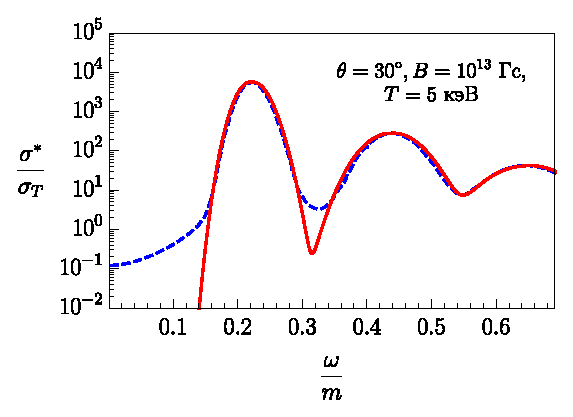
\includegraphics[width=0.32\linewidth,clip]{AliceDeltaAverageB023T001Deg30.eps}
	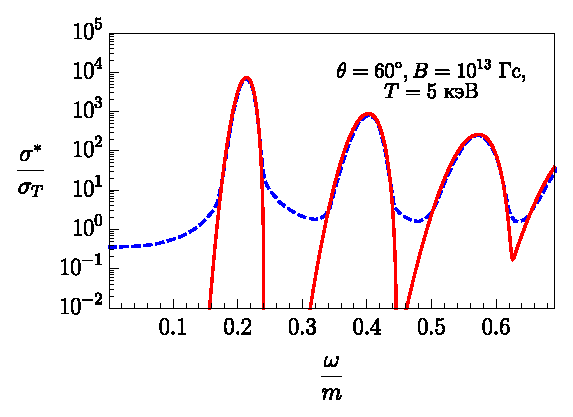
\includegraphics[width=0.32\linewidth,clip]{AliceDeltaAverageB023T001Deg60.eps}
	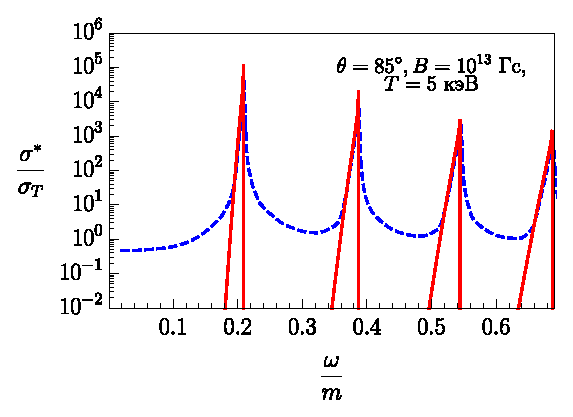
\includegraphics[width=0.32\linewidth,clip]{AliceDeltaAverageB023T001Deg85.eps}
	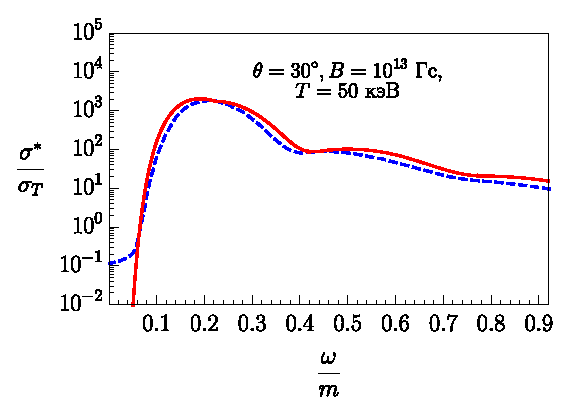
\includegraphics[width=0.32\linewidth,clip]{AliceDeltaAverageB023T01Deg30.eps}
	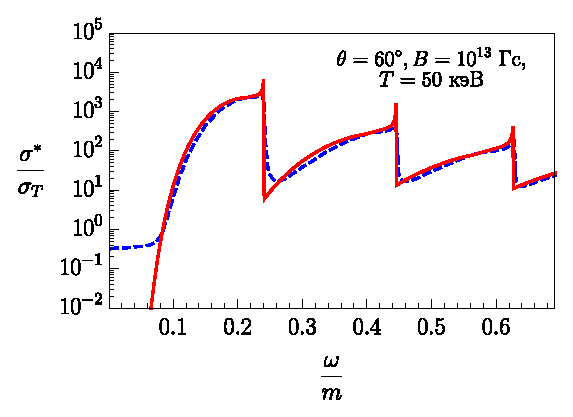
\includegraphics[width=0.32\linewidth,clip]{AliceDeltaAverageB023T01Deg60.eps}
	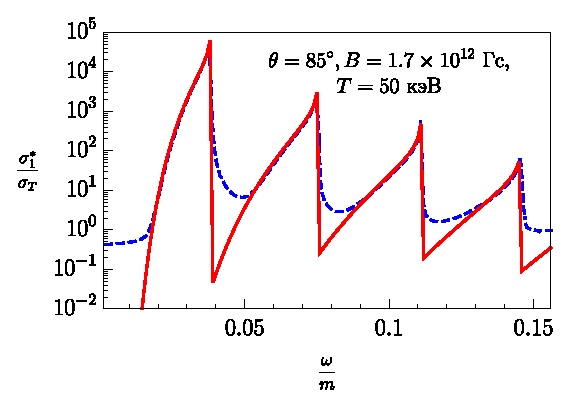
\includegraphics[width=0.32\linewidth,clip]{AliceDeltaAverageB023T01Deg85.eps}
	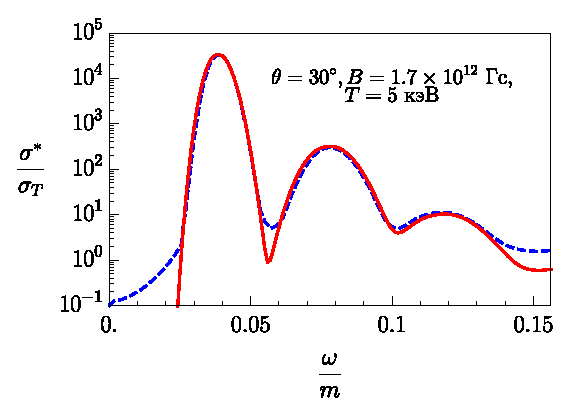
\includegraphics[width=0.32\linewidth,clip]{AliceDeltaAverageB0039T001Deg30.eps}
	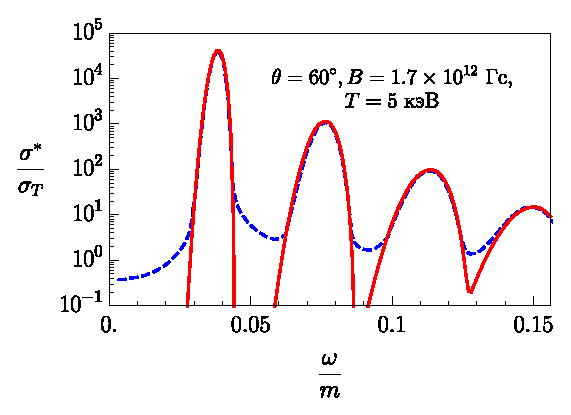
\includegraphics[width=0.32\linewidth,clip]{AliceDeltaAverageB0039T001Deg60.eps}
	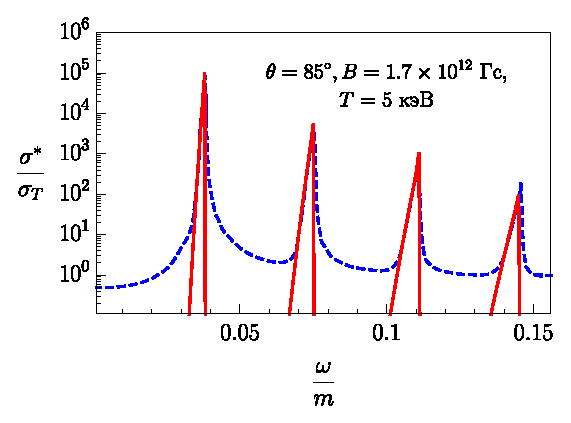
\includegraphics[width=0.32\linewidth,clip]{AliceDeltaAverageB0039T001Deg85.eps}
	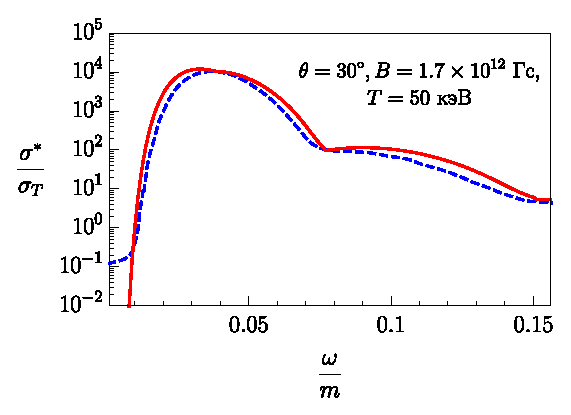
\includegraphics[width=0.32\linewidth,clip]{AliceDeltaAverageB0039T01Deg30.eps}
	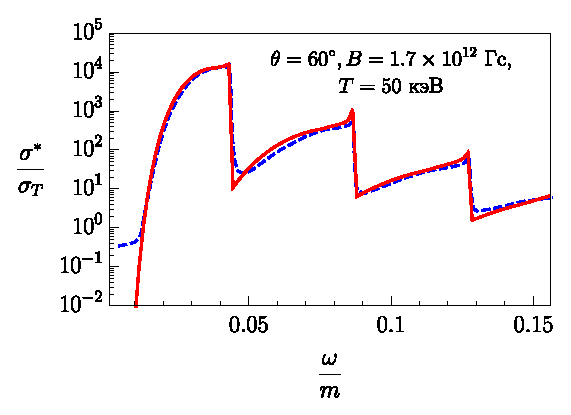
\includegraphics[width=0.32\linewidth,clip]{AliceDeltaAverageB0039T01Deg60.eps}
	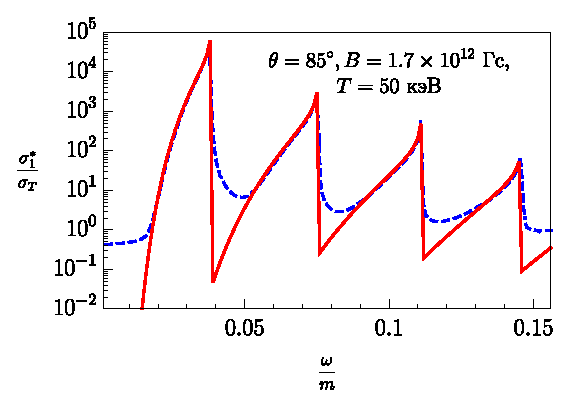
\includegraphics[width=0.32\linewidth,clip]{AliceDeltaAverageB0039T01Deg85.eps}	
	\caption{C������ (� �������� $\sigma_T$), ������������ �� ������������ ���������� ������, $e\gamma^{(2)}  \to e\gamma$, ���������� � ������~\cite{Harding:1991} (���������� �����) � $\delta$-�������������� ����������� (�������� �����) ��� ��������� ����� $\theta$ ����� ��������� ������ � ������������ ���������� ����. ��� ��������� � �������� ��������� ��������� �� �������� ������ ������.}
	\label{fig:CompAndHardO}
\end{figure}
\clearpage
\begin{figure}[t!]\centering
	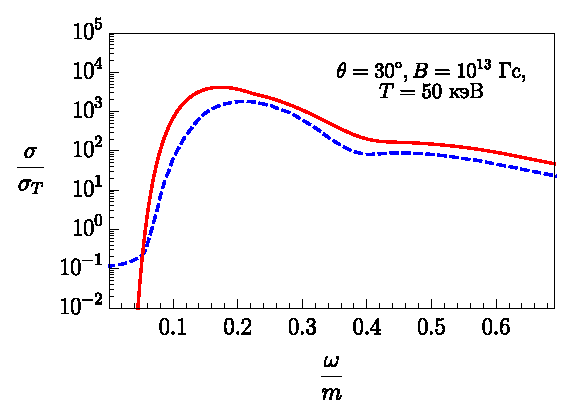
\includegraphics[width=0.55\linewidth,clip]{AliceDeltaManyLevelB023T01Deg30.eps}\\
	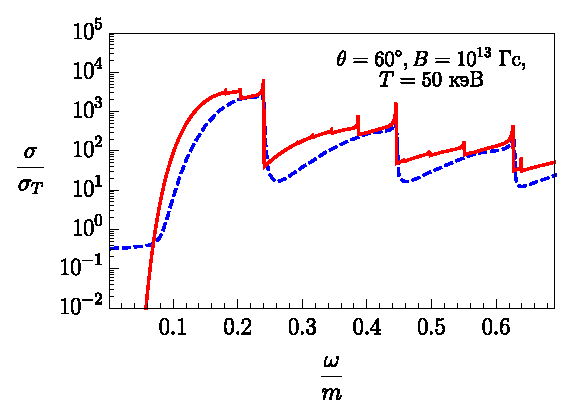
\includegraphics[width=0.55\linewidth,clip]{AliceDeltaManyLevelB023T01Deg60.eps}\\
	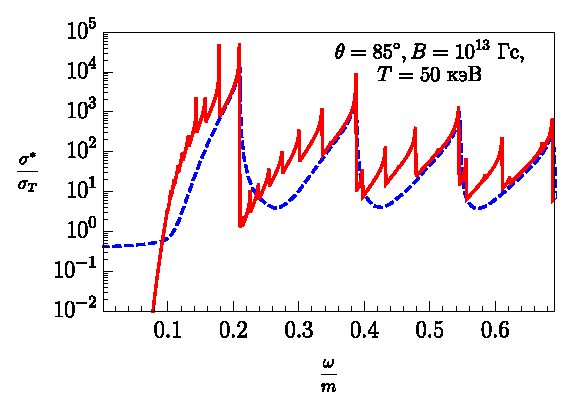
\includegraphics[width=0.55\linewidth,clip]{AliceDeltaManyLevelB023T01Deg85.eps}
	\caption{C������ (� �������� $\sigma_T$), ������������ �� ������������ ���������� ������ � �� ������������ ���������� ���������, $e\gamma^{(2)}  \to e\gamma$, ���������� � ������~\cite{Harding:1991} (���������� �����) � $\delta$-�������������� ����������� (�������� �����) ��� ��������� ����� $\theta$ ����� ��������� ������ � ������������ ���������� ����. �� ��������� ���������� ���. �������� ����������� $T=50$ ���, � ���������� ���� -- $B=10^{13}$ ��.\label{fig:HardingManyLevels}}
\end{figure}
\clearpage
��������� �������� ������� � ������ �������� ������, ������� ���� ����� �������� �� ����������� ������~\cite{Mushtukov:2016}, ����� ���������� �������� �� ���� ������� ������� ������� (��. ���.~\ref{fig:CompAndMushXGround}--\ref{fig:CompAndMushO}). ��������� ���������, ���������� � ���� ������, ������� �������������� ��������� ���� ��������� �~\cite{Schwarm:2017}, ��� ���� ���������� ��������� ���������� �~\cite{Schwarm:2017}  ��������� � ������������, ��������������� � ��������� �����������. ��� ����� ���� ������� � ���������� ������������ ��� ���������� �������� � ������~\cite{Mushtukov:2016}. \textcolor{red}{� ������� �� ������� ������ ������������ ��������.}


����� �������, ���������� 
�����������~(\ref{eq:delta_f}) ����������  � ������� ����� $B \sim 10^{12}-10^{15}$ ��, ����������� ��� ���������� � ��������������. � ������ �������, ���������� ������������ ���������� ������~(\ref{eq:wabs1}) �~(\ref{eq:wabs2}) ������������ ������ ��� ����� �������� ��������� (�� ����������� ��������� �����, ��������� �����), ��� �������� ������� ����� ������� � ����������� (��������, � ������� ������ �������� ���������), ��� ������ ���� �������� ������.
\clearpage
\begin{figure}[t!]\centering
	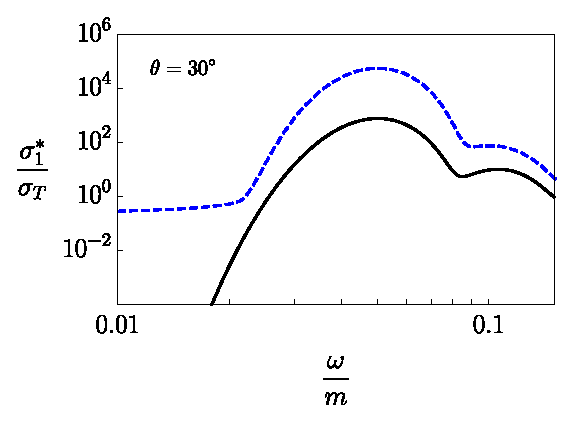
\includegraphics[width=0.5\linewidth,clip]{CompareMushOs005MushtukovX1Ground.eps}
	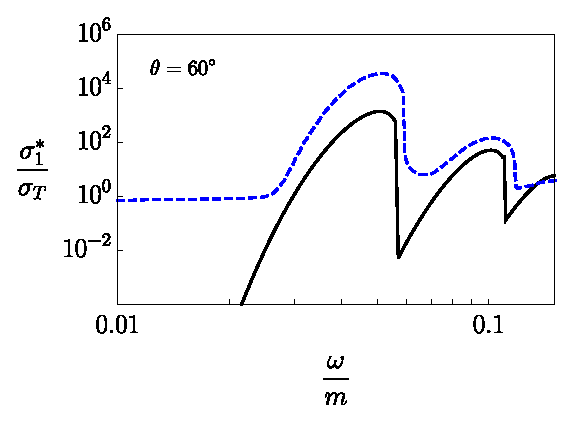
\includegraphics[width=0.5\linewidth,clip]{CompareMushOs005MushtukovX2Ground.eps}
	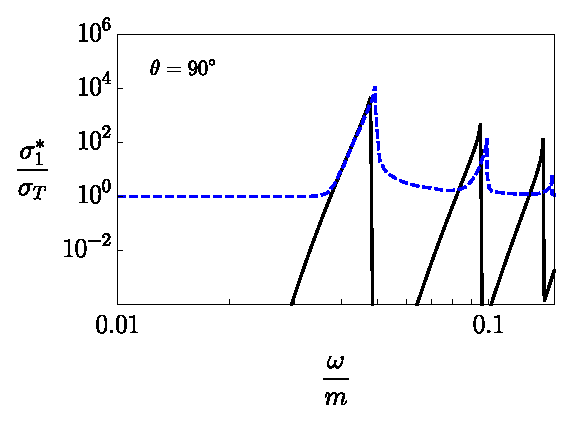
\includegraphics[width=0.5\linewidth,clip]{CompareMushOs005MushtukovX3Ground.eps}
	\caption{C������ (� �������� $\sigma_T$) ��������� ������ ���� 1, $e\gamma^{(1)}  \to e\gamma$, ���������� � ������~\cite{Mushtukov:2016} (���������� �����) � $\delta$-�������������� ����������� (�������� �����) ��� ��������� ����� $\theta$ ����� ��������� ���������� ������ � ������������ ���������� ���� (�������� ���������� �� ��������). $B=2.2\times 10^{12}$ ��, $T = 20$ ���, $\mu=0$. ��������� � �������� ��������� ��������� �� �������� ������ ������.}
	\label{fig:CompAndMushXGround}
\end{figure}
\begin{figure}[t!]\centering
	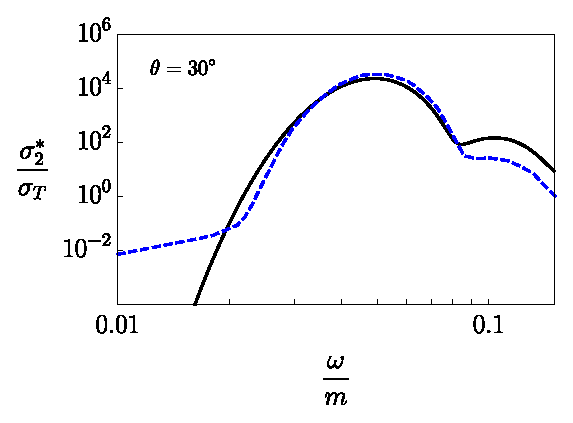
\includegraphics[width=0.5\linewidth,clip]{CompareMushOs005MushtukovO1Ground.eps}
	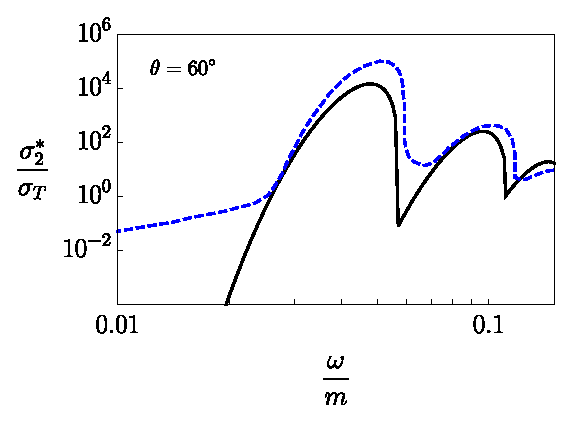
\includegraphics[width=0.5\linewidth,clip]{CompareMushOs005MushtukovO2Ground.eps}
	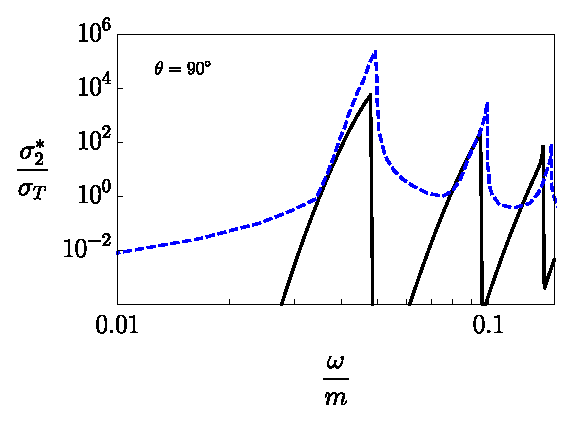
\includegraphics[width=0.5\linewidth,clip]{CompareMushOs005MushtukovO3Ground.eps}
	\caption{�� ��, ��� � �� ���.~\ref{fig:CompAndMushXGround} ��� ���������� ������ $B=2.2\times 10^{12}$ ��, $T = 20$ ���, $\mu=0$.}
	\label{fig:CompAndMushO}
\end{figure}
\clearpage



���������� ������ �������� ������������� ���������� ����, \linebreak\mbox{$B\sim 10^{15}-10^{16}$} �� � ������� ���������� $T=1$ ���, ������� ���������� ��� ���������� ������� SGR (���������� ������ ������������� �����-���������).  ������������ �������������� �������� � ��������� ����� ���������� �������� ���� ���������, ��������, � ������~\cite{Chistyakov:2009}. ������, ���������� � ���� ������������ ���������� ����� ������������� ������ ��� ������� ������� ������� ����� �� ����������. ������� ������������ ��������������� ������� ��������� ����������� ���������� ������ � ������� �������� ���� � ������ ���������� ��������� �� ����������� ��������� � �������� ������� ������������ ���� � �������� � ������������� ��������~\cite{Chistyakov:2009} � ������-�������������� ������������~\cite{RumShlenYar:2017}. ��������� � ������� �������� ���������� ���� ��������� � �������� ��������� ����� ��������������� �������� �������� ������� ������, � ����������� �������� -- ������ ������� ������, �� ����������� ���������� ������ � ������ �������� ������ ������������ ���� ������ ���������� ������� ��� ���������� ���. ��� ���� �������� � ������� 1.3, � ������� ��������� ���� ������� ������, �� ������� ����������� ��������, ����, ��� ����� �������� $e^+e^-$ ���� $q_{\mprl}^2=4m^2$ ��� ������ ���� 2 , �� ������������� ����������� ������ ������ ��������� $e\gamma^{(1)}\to e\gamma^{(1)}$ � $e\gamma^{(1)}\to e\gamma^{(2)}$. ������� ��������, ��� ��� ������ ����~1 ����� �������� $e^+e^-$ ���� $q_{\mprl}^2=(M_1+m)^2$ �������� ���� ��������������� ������� ��������� $q_{\mprl}^2=(M_1-m)^2$.

������ �� ����������� ������~\cite{Chistyakov:2009}, ���������� ����������� ��������� �������������� �������� � ������� �������� ���������� ���� � ����:
\begin{equation}\begin{gathered}\label{amplnonres}
		{\cal M}_{e\gamma^{(1)}\to e\gamma^{(1)}}=\frac{8i\pi\alpha m}{\beta}\frac{(q\varphi q')(q\tilde{\varphi}q')}{\sqrt{q^2_\perp q^{'2}_\perp (-Q^2_{\mprl})}}\, ,\\
		{\cal M}_{e\gamma^{(1)}\to e\gamma^{(2)}}=\frac{8i \pi\alpha m}{\beta}\frac{(q\Lambda q')(q\tilde{\Lambda} Q)}{\sqrt{q^2_\perp {q'}^2_{\mprl}(-Q^2_{\mprl})}}\, ,\hspace{2mm} 
\end{gathered}\end{equation}
���   
$Q^2_{\mprl} = (q - q')^2_{\mprl} <0$,
$q_{\alpha} = (\omega,{\bf k})$ � $q'_{\alpha} = (\omega',{\bf k'})$
-- 4-�������� ���������� � ��������� ������� ��������������.

����� ����������� (\ref{amplnonres}) �
(\ref{eq:WabsStrongB}) ������������ ���������� ������ ��� ������� $e\gamma^{(1)}\to e\gamma^{(1)}$ � $e\gamma^{(1)}\to e\gamma^{(2)}$ � ������������� ������� ��� �������, ������������������ ��� ����� $\theta=90^\circ$ �� ��������� � ����������� ���������� ����,  ����� ���� ������������ ��������� �������:
\begin{equation}\label{Wnonres}\begin{aligned}
		W_{e\gamma^{(1)}\to e\gamma^{(1)}}&=\frac{\omega \alpha^2m^2}{2 \beta \pi}\int dQ_0 dk_z' \frac{{k_z'}^2}{(-Q_{\mprl}^2)^2\varkappa}\theta(-Q_{\mprl}l^2)
		\theta({q'}_{\mprl}^2)\times\\&\times \sum_{\sigma} f(E_\sigma)(1-f(E_\sigma+\omega))(1+f_{\omega'})\, ,
\end{aligned}\end{equation}
\begin{equation}
	\begin{aligned}\label{Wnonres2}
		W_{e\gamma^{(1)}\to e\gamma^{(2)}}&=\frac{ \alpha^2m^2}{2 \beta \pi \omega}\int dQ_0 dk_z'\left(1-\frac{{\cal P}^{(2)}(q')}{{q'}_{\mprl}^2}\right) \frac{{q'}_{\mprl}^2-\omega\omega'}{(-Q_{\mprl}^2)^2\varkappa}\theta(-Q_{\mprl}^2)
		\theta({q'}_{\mprl}^2)\times\\ &\times\sum_{\sigma} f_{E_\sigma}(1-f_{E_\sigma+\omega})(1+f_{\omega'})\, ,
	\end{aligned}
\end{equation}
\noindent ��� $\theta(x)$ -- ������� ���������,
\mbox{$\varkappa = \sqrt{1 - 4m^2/Q^2_{\mprl}}$, $E_\sigma=\sqrt{p_{z\sigma}^2+m^2}$}, � \linebreak $p_{z\sigma}$ -- ����� ��������� $Q_0+E_\sigma-E'_\sigma=0$:
\begin{equation}\label{savelaw}
	p_{z\sigma}=-\frac{Q_z}{2}+ \sigma Q_0 \varkappa\, .
\end{equation} 

���������������� ������������ ������~\cite{Chistyakov:2009}, ��������� ${\cal M}_{e\gamma^{(1)}\to e\gamma^{(1)}}$, ${\cal M}_{e\gamma^{(1)}\to e\gamma^{(2)}}$ � ������� �������� ���������� ���� � � ������ �������� ������ ������������ ���� ����� ����������� ��������� �������:
\begin{equation}\label{Mres}
	\begin{aligned}
		{\cal M}_{e\gamma^{(1)}\to e\gamma^{(1)}}=& \frac{8m\pi\alpha}{\sqrt{(-Q^2_{\mprl})}} \exp\left[-\frac{q^2_\perp+q'^2_\perp-2i(q\varphi q')}{4\beta}\right]\cdot\frac{1}{\sqrt{q^2_\perp q'^2_\perp}}\times 
		\\ &\times \sum_{n=1}^{\infty}\frac{((q\Lambda
			q')-i(q\varphi
			q'))^{n}}{(n-1)!(2\beta)^{n-1}}
		\frac{(q\tilde{\varphi}q')}{(p+q)^2_{\mprl}-M_n^2+iE''_n\Gamma_n }+\\
		&+(q\leftrightarrow-q')\, ,
	\end{aligned}
\end{equation}
\begin{equation}\label{Mres12}
	\begin{aligned}
		{\cal M}_{e\gamma^{(1)}\to e\gamma^{(2)}}=& \frac{8m\pi\alpha}{\sqrt{(-Q^2_{\mprl})}} \exp\left[-\frac{q^2_\perp+q'^2_\perp-2i(q\varphi q')}{4\beta}\right]\cdot\frac{1}{\sqrt{q^2_\perp q'^2_{\mprl}}}\times 
		\\ &\times \sum_{n=1}^{\infty}\frac{((q\Lambda
			q')-i(q\varphi
			q'))^{n}}{(n-1)!(2\beta)^{n-1}}
		\frac{(Q\tilde{\Lambda}q')}{(p+q)^2_{\mprl}-M_n^2+iE''_n\Gamma_n }+\\
		&+(q\leftrightarrow-q')\, ,
	\end{aligned}
\end{equation}
��� ������ ������ ���������� ��������� $\Gamma_n$  �������� ����������~(\ref{eq:weldon}).� ������ �������, ��� ���������� ��������� ������, � ������ ������ �������������, �������, ��������-������������ ������ ������ ������ ���������� ��������� ���� ���������� �� ���������������� ��������� � ������� ��������� ���� � �������������������� ����������~\cite{KM_Book_2013}:
\begin{equation}\label{Shir}
	\begin{aligned}
		E''_n\Gamma_n=&\alpha \beta \sum_{n'=0}^{n-1}\int_{0}^{(\sqrt{n}-\sqrt{n'})^2}\frac{dx}{\sqrt{(n+n'-x)^2-4n n'}}\times\\
		&\times\{(n+n'-x)[{\cal I}^2_{n,n'-1}(x)+{\cal I}^2_{n-1,n'}(x)]-\\
		&-4\sqrt{nn'}{\cal I}_{n,n'}(x){\cal I}_{n-1,n'-1}(x)\}\, ,
	\end{aligned}
\end{equation}
��� $E''_n=E+\omega$ -- ������� ������������ ���������.

 ����������� ������������ ���������� ������ ��� �������\linebreak $e \gamma^{(1)} \to e\gamma^{(1)}$ � $e \gamma^{(1)} \to e\gamma^{(2)}$ � ������ �������� ������ ���������� ��������� ����� ���� �������� ������������ ��������~(\ref{Mres}) �~(\ref{Mres12}) �~(\ref{eq:WabsStrongB}) � � ������, ����� ��������� ����� ���������������� ������� ���������� ����, ������������ ���������� ����� ����������� ��������� �������:


\begin{equation}
	\begin{aligned}\label{Wres}
		&W_{e\gamma^{(1)}\to e\gamma^{(1)}}=\frac{\beta\alpha^2m^2}{\pi} \int dQ_0dk'_z \frac{{k_z'}^2\omega } {(-Q_{\mprl}^2)^2\varkappa}\exp\left[-\frac{\omega^2+{q'}_\perp^2}{2\beta}\right]\times\\ 
		&\times\sum_{n=1}^{\infty}\sum_{\sigma=\pm 1}\frac{1}{[(n-1)!]^2}\left(\frac{\omega \sqrt{q_\perp'^2}}{2\beta}\right)^{2(n-1)}\bigg\{
		\frac{1}{((p_\sigma+q)_{\mprl}^2-M_n^2)^2+(E''_n\Gamma_n)^2}  +\\
		&+\frac{1}{((p_\sigma-q')_{\mprl}^2-M_n^2)^2+(E''_n\Gamma_n)^2}-
		\\
		&-2
		\sum_{n'=1}^{\infty}\frac{(n-1)!}{(n'-1)!}\left(\frac{\omega \sqrt{q_\perp'^2}}{2\beta}\right)^{n'-n}J_{n+n'}\left(\frac{\omega \sqrt{q_\perp'^2}}{\beta}\right)\times\\
		&\times\frac{[(p_\sigma+q)^2_{\mprl}-M_n^2][(p_\sigma-q')^2_{\mprl}-M^2_{n'}]+E''_n\Gamma_nE''_{n'}\Gamma_{n'}}{[((p_\sigma-q')_{\mprl}^2-M_n^2)^2+(E''_n\Gamma_n)^2][((p_\sigma+q)_{\mprl}^2-M_{n'}^2)^2+(E''_n\Gamma_{n'})^2]}
		\bigg\}\times
		\\&\times f_{E_\sigma}(1-f_{E_\sigma+Q_0})(1+f_{\omega'}
		) \, ,
	\end{aligned}
\end{equation}

\begin{equation}
	\begin{aligned}\label{Wres2}
		&W_{e\gamma^{(1)}\to e\gamma^{(2)}}=\frac{\beta\alpha^2m^2}{\pi} \int dQ_0dk'_z \frac{q_\perp'^2\omega } {(-Q_{\mprl}^2)^2\varkappa}\exp\left[-\frac{q_\perp^2+{q'}_\perp^2}{2\beta}\right]\times\\ 
		&\times\sum_{n=1}^{\infty}\sum_{\sigma=\pm 1}\frac{1}{[(n-1)!]^2}\left(\frac{\omega \sqrt{q_\perp'^2}}{2\beta}\right)^{2(n-1)}\bigg\{
		\frac{Q_0/\omega}{((p_\sigma+q)_{\mprl}^2-M_n^2)^2+(E''_n\Gamma_n)^2}+
		\\
		&+\frac{Q_0^2/q'^2_{\mprl}}{((p_\sigma-q')_{\mprl}^2-M_n^2)^2+(E''_n\Gamma_n)^2}-
		\\
		&-2
		\sum_{n'=1}^{\infty}\frac{(n-1)!}{(n'-1)!}\left(\frac{\omega \sqrt{q_\perp'^2}}{2\beta}\right)^{n'-n} J_{n+n'}\left(\frac{\omega \sqrt{q_\perp'^2}}{\beta}\right)\times\\
		&\times\frac{[(p_\sigma+q)^2_{\mprl}-M_n^2][(p_\sigma-q')^2_{\mprl}-M^2_{n'}]+E''_n\Gamma_nE''_{n'}\Gamma_{n'}}{[((p_\sigma-q')_{\mprl}^2-M_n^2)^2+(E''_n\Gamma_n)^2][((p_\sigma+q)_{\mprl}^2-M_{n'}^2)^2+(E''_n\Gamma_{n'})^2]}
		\times\\&\times
		\frac{Q_0^2(\omega-Q_0)}{\omega q'^2_\perp}
		\bigg\}\times f_{E_\sigma}(1-f_{E_\sigma+Q_0})(1+f_{\omega'}
		) \, ,
	\end{aligned}
\end{equation}
\noindent ��� $J_n(x)$ -- ������� ������� ������ �������, $p^\alpha_{\sigma\mprl}=(E_\sigma,p_{z\sigma})$. ���������� ������������ �������� ��������� ������ ������������ �� ��������� ���������:
\begin{equation}
	q'^2_{\mprl}=q'^{2}_\perp + {\cal P}^{(\lambda)}(q') .
\end{equation}

����� ����� �������� ������������� ������ ����������� ������ \cite{Chistyakov:2009}  � ����������� ������� (\ref{Wres}) � (\ref{Wres2}) ��� ��������-������������ ������ � ����������� ����������� ��������������� �������� ������ �� ��������� � �������� ���������� ���� ��� ��������� �������� �������� ���������� ����, ����������� � ������� ���������� ������.



�� ���.~\ref{Graph11B200T1}--\ref{Graph11B20T1} �������  ����������� ���������� $W_{1\to1}$ ��������� ��� ����������� $T=1 $~��� � �������� ���������� ���� $B=200B_e$ � $B=20B_e$ ��������������. ��� ����� �� ���.~\ref{Graph11B200T1}--\ref{Graph11B20T1}, ����������� ���������� ��� ������ $\gamma^{(1)}e\to\gamma^{(1)}e$ ����������� � ���������������� ������������ ��� ������� �������� ���� � ���������� ���������, ����������� � ������ \cite{Chistyakov:2009} ������ �� ������� ���������� ������  $\omega\simeq3$~��� ��� ���� $B=200B_e$ �  $\omega\simeq0.3$~��� ��� ���� $B=20B_e$. ������ �������� ����������� �� ������������ ����������� ������ \cite{Chistyakov:2009} �� �������� ���������� ������. ����������� �������� ����������� � ��� ������ $\gamma^{(1)}e\to\gamma^{(2)}e$ (��. ���. \ref{Graph12B200T1}--\ref{Graph12B20T1}).  �� ���. \ref{Graph11B20T1} � \ref{Graph12B20T1} �������� ���� ����� ��������� ������������ ���������� ���� ��� ������������ ����� �������� ���������� ������. ���� ���� ������ � ���, ��� � ������� �������� ���������� ���� ���������� ��������� �������������� �������� �� �������� �������� ���� ��� �� ����� �����������.  

������� ��������   ��� ��� ������������ ����� ������������ $T\lesssim50$ ��� � ��� �� ��������� ����� $\delta$-������������� �������� ���� ��-�� ���������� ������� ���������. � ����� $\delta$-�������������� ����������� ���������� ������ ��������� ���� ������ ����������� ���.

������� ��������   ��� ��� ������������ ����� ������������ $T\lesssim50$ ��� � ��� �� ��������� ����� $\delta$-������������� �������� ���� ��-�� ���������� ������� ���������. � ����� $\delta$-�������������� ����������� ���������� ������ ��������� ���� ������ ����������� ���.
\clearpage
\begin{figure}[t!]\centering
	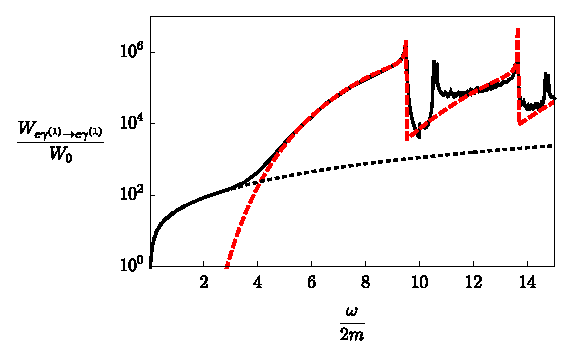
\includegraphics[width=0.8\linewidth]{Splot112001.eps}
	\caption{����������� ������������ ���������� �� ������� ���������� ������ ��� ������ $e\gamma^{(1)}\to e\gamma^{(1)}$ ��� ���� $B=200 B_e$ � ����������� T=1 ���: �������� ����� -- ����������� ���������� � ������ ���������; ��������� ����� -- ��� ����� ���������; ���������� ����� -- ������-�������������� �����������. ����� $W_0=(\alpha/\pi)^3m\simeq 3.25\cdot10^2$ ��$^{-1}$.}
	\label{Graph11B200T1}
\end{figure}

\begin{figure}[t!]\centering
	\includegraphics[width=0.8\linewidth]{Splot11201.eps}
	\caption{����������� ������������ ���������� �� ������� ���������� ������ ��� ������ $e\gamma^{(1)}\to e\gamma^{(1)}$ ��� ���� $B=20 B_e$ � ����������� T=1 ���. ����������� ��� ����� �� ��, ��� � ��� ���. \ref{Graph11B200T1}.}
	\label{Graph11B20T1}
\end{figure}

\begin{figure}[t!]\centering
	\includegraphics[width=0.8\linewidth]{Splot122001.eps}
	\caption{����������� ������������ ���������� �� ������� ���������� ������ ��� ������ $e\gamma^{(1)}\to e\gamma^{(2)}$ ��� ���� $B=200 B_e$ � ����������� T=1 ���. ����������� ��� ����� �� ��, ��� � ��� ���. \ref{Graph11B200T1}.}
	\label{Graph12B200T1}
\end{figure}

\begin{figure}[t!]\centering
	\includegraphics[width=0.8\linewidth]{Splot12201.eps}
	\caption{����������� ������������ ���������� �� ������� ���������� ������ ��� ������ $e\gamma^{(1)}\to e\gamma^{(2)}$ ��� ���� $B=20 B_e$ � ����������� T=1 ���. ����������� ��� ����� �� ��, ��� � ��� ���. \ref{Graph11B200T1}.}
	\label{Graph12B20T1}
\end{figure}
\clearpage

\subsection{Резонансное рождение аксионов в магнитосфере магнитара}

Как было отмечено во Введении к настоящей диссертации, аксион, предложенный Печчеи  и Куинн~\cite{Quinn:1977} для 
решения проблемы сохранения CP инвариантности 
сильных взаимодействий, остается в настоящее время не только самым привлекательным 
решением проблемы CP, но и наиболее вероятным кандидатом на роль холодной темной
материи Вселенной. Поскольку масштаб нарушения симметрии Печчеи-Куинн, $f_a$,
оказывается велик, аксионы очень слабо взаимодействуют с веществом
(константа взаимодействия $f_a^{-1} \lesssim 10^{-8}$\, ГэВ$^{-1}$~\cite{Raffelt:1996}). 
В этой связи возникают определенные трудности
на пути экспериментального обнаружения аксиона.

Как уже неоднократно отмечалось ранее, влияние внешней активной среды на реакции с 
участием элементарных частиц и, в частности,  аксионов,
в зависимости от значений параметров среды (температуры  $T$, 
химического потенциала  $\mu$ или индукции магнитного поля  $B$), может
 как катализировать эти реакции, так и оказывать дополнительное (к $f_a^{-1}$) 
их подавление.  

%
\begin{figure}
\centerline{\includegraphics[width=5cm]{fig5_1.eps}}
\caption{Диаграммы Фейнмана для процесса общего вида $i \to 
f+a$. Двойные линии означают, что влияние внешнего поля на начальное и 
конечное состояния учтено точно.}
\label{fig:Diagaxion}
\end{figure}


В таких условиях представляет интерес рассмотреть процесс рождения аксионов   в 
реакции общего вида $i \to f + a$ (диаграмма на рис.~\ref{fig:Diagaxion}), 
где в начальном ($i$) и конечном ($f$) состояниях могут присутствовать 
заряженные компоненты среды. 
На рис.~\ref{fig:Diagaxion} зачерненный
кружок обозначает эффективную вершину $\gamma a$ взаимодействия
(диаграммы на рис.~\ref{fig:vertexaxion}). Нетрудно видеть, что из-за наличия виртуального 
фотона рассматриваемый процесс может иметь резонансный характер. Похожая ситуация
для области, близкой к резонансу, была рассмотрена в работе~\cite{Skobelev:2007} 
на примере
комптоновского рассеяния реликтовых фотонов на электронах и позитронах магнитосферы
магнитара. Однако, как будет показано ниже,  результаты, полученные 
в~\cite{Skobelev:2007}, являются неточными. 

\begin{figure}
\centerline{\includegraphics[width=15cm]{fig5_2.eps}}
\caption{ Диаграммы Фейнмана для эффективной вершины $\gamma a$ 
взаимодействия.}
\label{fig:vertexaxion}
\end{figure}



 В существующих аксионных моделях и в присутствии 
внешнего магнитного поля процесс  $i \to f+a$ 
можно описать эффективным лагранжианом вида~\cite{Raffelt:1996} 
(см. также формулы~(\ref{eq:Lel}) и~(\ref{eq:Laxion}) главы~\ref{Sec:1}):
%
\begin{eqnarray}
\label{eq:L1}
&&{\cal L}_{a\gamma}(x) = g_{a\gamma}\tilde F^{\mu \nu} [\partial_{\nu}A_{\mu}(x)] a(x) + 
\\
\nonumber
&& + \frac{g_{af}}{2m_f} 
[\bar \psi_f(x) \gamma^{\mu} \gamma_5 \psi_f(x)] \partial_{\mu} a(x) - 
%\\
%\nonumber
%&+&
 e_f[\bar \psi_f(x) \gamma^{\mu} \psi_f(x)]A_{\mu}(x) \, .
\end{eqnarray}
%
\noindent Напомним, что  $A_{\mu}$ -- четырехмерный потенциал квантованного электромагнитного
поля, $\tilde F^{\mu \nu}$ --  дуальный тензор внешнего поля,  $\psi_f(x)$  и $a(x)$ --  
квантованные фермионное и аксионное поля, 
  $g_{a\gamma} = \alpha \zeta/2\pi f_a$, $\zeta$ --  модельно зависимый 
параметр порядка единицы, 
$g_{af} = C_f m_f/f_a$ -- безразмерная Юкавская константа связи аксионов с 
фермионами с модельно зависимым фактором $C_f$, $e_f$ -- электрический заряд 
фермиона (для электрона $e_f = - e$). 

Исходя из лагранжиана~(\ref{eq:L1}) амплитуда процесса $i \to f + a$ может быть
представлена в следующем виде 
%
\begin{equation}
{\cal M}^a_{i \to f} 
 = - \frac{{\cal M}^{\gamma}_{if} {\cal M}_{\gamma \to a}}
{q'^2 -\varkappa^{(\varepsilon)}(q')}\, , 
\label{eq:M1if}                                                       
\end{equation}
%
\noindent где ${\cal M}^{\gamma}_{if}$ -- амплитуда процесса $i \to f + \gamma$  с 
излучением фотона в конечном состоянии,
%
\begin{equation}
{\cal M}_{\gamma \to a} 
 = i \bar g_{a\gamma} (\varepsilon \tilde F q') 
\label{eq:M2}                                                       
\end{equation}
%
\noindent --  амплитуда перехода фотон $\to$ аксион,  $q'^{\mu} = (\omega',{\bf k}')$ --   
четырехмерный импульс аксиона, $\varkappa^{(\varepsilon)}(q')$ -- собственное значение 
 поляризационного  оператора
фотона, которому соответствует вектор поляризации $\varepsilon_{\alpha}$. Эффективную  
константу аксион-фотонного взаимодействия, $\bar g_{a\gamma}$, можно 
представить в виде трех слагаемых: $\bar g_{a\gamma} = g_{a\gamma} + 
\Delta g^{B}_{a\gamma} + \Delta g^{pl}_{a\gamma}$.    
 Первое слагаемое соответствует взаимодействию 
аксиона с электромагнитным полем, обусловленному аномалией 
Адлера (диаграмма (a) на рис.~\ref{fig:vertexaxion}), второе обусловлено 
взаимодействием аксиона  с фотоном через электронную петлю 
(диаграмма (b) на рис.~\ref{fig:vertexaxion}), а третье --   
рассеянием вперед на электронах и позитронах плазмы (диаграммы (c) и (d) 
на рис.2). Подробный расчет $\Delta g^{B}_{a\gamma}$ и
$\Delta g^{pl}_{a\gamma}$ был сделан ранее в работах~\cite{Mikheev:1999} 
и~\cite{Mikheev:2006} соответственно. 
 Здесь мы отметим только, что для корректного вычисления величины $\Delta g^{B}_{a\gamma}$  
в ней необходимо 
 произвести вычитание, соответствующее аномалии Адлера~\cite{Mikheev:1999}. 
Этот факт, в 
частности, не был учтен в работе~\cite{Skobelev:2007}, что является одной из причин  
ошибочности полученных там результатов.

Далее представим $\varkappa^{(\varepsilon)}(q')$ в виде    
$\varkappa^{(\varepsilon)} = \Re - i\Im$, 
где $\Re = Re (\varkappa)$  реальная, а $\Im =  Im (\varkappa)$  мнимая части 
поляризационного оператора. Последняя обусловлена процессами поглощения и 
излучения фотонов в плазме и,
согласно~\cite{Weldon:1983}, следующим образом выражается через полную 
ширину рождения фотона, $\Gamma_{cr}$: 
%
\begin{eqnarray}
\label{eq:I1}                                                       
\Im = \omega' \left (e^{\omega'/T} - 1 \right ) \Gamma_{cr} ,  \quad 
%\\
%\nonumber 
\Gamma_{cr} = \sum_{i,f} \int  |{\cal M}^{\gamma}_{if}|^2 d\Phi_{if} ,
\end{eqnarray}
%
\noindent где $d\Phi_{if}$ --  элемент фазового объема состояний $i$ и $f$ для процесса 
$i \to f + \gamma$ с учетом соответствующих функций распределения,  
и сумма берется по всем возможным начальным и конечным состояниям. 

С учетом вышесказанного, аксионная светимость за счет всевозможных реакций с участием 
частиц плазмы может быть представлена  в виде 
%
\begin{equation}
Q = \sum_{i,f} \int d\Phi_{if} \, d\Phi' \, \omega' 
|{\cal M}^{\gamma}_{if}|^2 \, ,
\label{eq:Qa0}                                                       
\end{equation}
%
\noindent где $d\Phi' = \frac{d^3 k'}{(2\pi)^3 2 \omega'}$  фазовый объем аксиона. 

С учетом~(\ref{eq:M1if}) и~(\ref{eq:I1}) $Q$ примет вид
%
\begin{equation}
Q = \int  \frac{d\Phi' \, |{\cal M}_{\gamma \to a}|^2}{e^{\omega'/T} - 1} \, 
\frac{\Im
} 
{(q'^2 -\Re)^2 + \Im^2} \, .
\label{eq:Qa1}                                                       
\end{equation}
%

Как видно из~(\ref{eq:Qa1}), наиболее существенный вклад в аксионную светимость будет
давать область резонанса, т.е. окрестность точки пересечения дисперсионных кривых
аксиона $q'^2 = m_a^2$ и фотона, $q'^2 = \Re$, так 
что фотон становится реальным. В окрестности резонанса часть подынтегрального выражения
в~(\ref{eq:Qa1}) можно интерполировать $\delta$-функцией:  
%
\begin{equation}
 \frac{\Im}
{(q'^2 -\Re)^2 + \Im^2} \simeq \pi \, \delta(q'^2 -\Re) \, .
\label{eq:Del1}
\end{equation}
%
\noindent Воспользовавшись свойствами $\delta$-функции, перепишем~(\ref{eq:Del1})
 в виде  
%
\begin{equation}
 \frac{\Im}
{(q'^2 -\Re)^2 + \Im^2} \simeq \pi \, 
\int \frac{d^3 k}{2 \omega} Z_{\varepsilon} \delta^4 (q-q') \, ,
\label{eq:Del2}
\end{equation}
%
\noindent где  $Z_{\varepsilon}^{-1} = 1-\frac{\partial \Re}{\partial \omega^2}$ 
соответствует перенормировке волновой функции фотона.


 С учетом~(\ref{eq:Del2}) cветимость~(\ref{eq:Qa1}) примет вид 
%
\begin{eqnarray}
\label{eq:Qa2}
Q &\simeq&  (2\pi)^4 \, 
\int \frac{d^3 k}{2 \omega (2\pi)^3} \,\frac{\omega}{e^{\omega/T} - 1} \times
\\
\nonumber 
&\times& \int \frac{d^3 k'}{2 \omega' (2\pi)^3}\, Z_{\varepsilon} 
|{\cal M}_{\gamma \to a}|^2 \delta^4 (q-q') \, .
\end{eqnarray}
%
\noindent Полученное выражение в точности соответствует формуле для аксионной светимости  
в процессе $\gamma \to a$. Таким образом, аксионная светимость в 
области резонанса за счет всевозможных  
реакций с участием частиц среды 
  однозначно выражается через светимость перехода фотон $\to$ 
аксион.


После интегрирования с $\delta$-функциями светимость приводится к виду
%
\begin{eqnarray}
Q =  \frac{\bar g_{a\gamma}^2 (\beta)^2}{32 \pi^2 \alpha} \, 
\int_{-1}^1 \frac{dx}{e^{\omega/T}-1} \, 
\frac{Z_{\varepsilon} k 
(\varepsilon \tilde \varphi q)^2}{\left |1-\frac{d\omega^2}{dk^2}\right |}\bigg |_{k=k^*}\, .
\label{eq:Qa3}
\end{eqnarray}
%

\noindent Здесь $x = \cos{\theta}$, $\theta$ --  угол 
между направлением импульса фотона и магнитным полем, $k^* = k^*(\theta)$ --  
 корень уравнения $\omega^2 (\vec k) = m_a^2+k^2$. 
% $\tilde \varphi_{\alpha \beta} = \tilde F_{\alpha \beta}/B$.


Дальнейшее вычисление светимости будет существенно зависеть от характеристик плазмы, 
определяющих, в конечном итоге, дисперсионные свойства фотонов. Здесь мы остановимся 
на двух частных случаях.

i) Слабо замагниченная плотная плазма,  $m_a^2 \ll \beta \ll T^2 , \mu^2$. В этом 
случае в качестве $\varepsilon_\alpha$ будет выступать вектор поляризации продольного 
плазмона
%
\begin{eqnarray}
\varepsilon_\alpha = \sqrt{\frac{q^2}{(uq)^2-q^2}}\, 
\left (u_\alpha - \frac{(uq)}{q^2}\, q_\alpha \right ) , 
\end{eqnarray}
%
где $u_\alpha$ -- 4-скорость плазмы. Светимость~(\ref{eq:Qa3}) примет простой вид
%
\begin{eqnarray}
Q =  \frac{\bar g_{a\gamma}^2 (\beta)^2}{48 \pi^2 \alpha} \, 
 \frac{(k^*)^3}{e^{k^*/T}-1} \, 
\label{eq:Qa4}
\end{eqnarray}
%

\noindent 
в полном согласии с результатом работы~\cite{MRV:1998}. Отметим, что в данном пределе 
 величина $k^*$ не зависит от $\theta$, а определяется только параметрами плазмы.


ii) Сильно замагниченная нерелятивистская холодная плазма  $\beta \gg m^2$, $\mu^2 \gg T^2$. Здесь %\newline   
$\varepsilon_\alpha = 
(q \tilde \varphi)_\alpha/\sqrt{q^2_{\mprl}}$, 
$\Re \simeq (q \tilde \varphi \tilde \varphi q) \left (\frac{\omega_p^2(1+\xi)}{\omega^2} -
\xi \right )$, и плазменная частота $\omega_p$   
следующим образом связана с концентрацией электронов:  $\omega^2_p = 4\pi \alpha n/m$; $\xi = (\alpha/3\pi)(B/B_e)$. 
Кроме того, в рассматриваемом пределе 
$\bar g_{a\gamma} \simeq g_{a\gamma}$. Однако,  
в отличие от случая слабо замагниченной плазмы, светимость до конца интегрируется
лишь в некоторых частных случаях:

\begin{itemize} 

\item масса аксиона --  наименьший параметр задачи, т.е. 
$\omega_p, \,T \gg m_a$ (например, рождение легких, с массой меньшей, чем 
$10^{-5}$\,эВ, аксионов в магнитосфере
магнитара).  % (см. формулу~(\ref{eq:n1}))). 
В этом случае 
$k^* \simeq \omega_p \sqrt{1+1/\xi}$ и светимость~(\ref{eq:Qa3}) примет вид
%
\begin{eqnarray}
\label{eq:Qa5a}
Q &\simeq&  \frac{g_{a\gamma}^2 (\beta)^2}{16 \pi^2 \alpha} \,
\omega_p^3 \frac{(1+\xi)^{3/2}}{\xi^{5/2}}\times
\\
\nonumber 
&\times& \left (\exp{\left [\frac{\omega_p}{T} 
\sqrt{1+\frac{1}{\xi}}\, \right ]}-1 \right )^{-1} \, .
\end{eqnarray}
%


\item $\omega_p \gg T \sim m_a$. Анализ показывает, что в этом 
случае интеграл в~(\ref{eq:Qa3}) набирает
свою величину в области $x\simeq 1$, и, следовательно, $k^* \simeq \omega_p $.
  Тогда светимость примет вид
%
\begin{eqnarray}
\label{eq:Qa5b}
Q &\simeq&  \frac{g_{a\gamma}^2 (\beta)^2}{16 \pi^2 \alpha} \, T m_a^2  \, 
e^{-\omega_p/T} \, .
\end{eqnarray}
%

\end{itemize}

Кроме светимости представляет самостоятельный интерес оценка количества аксионов,
рождаемых в магнитосфере магнитара в единице объема за единицу времени с 
помощью рассмотренного выше резонансного
механизма, поскольку аксион является одним из основных кандидатов в составляющие
холодной темной материи. Аналогично~(\ref{eq:Qa3}), (\ref{eq:Qa5a}) 
и~(\ref{eq:Qa5b}) получаем: 
%
\begin{eqnarray}
\frac{dN}{dt dV} =  \frac{g_{a\gamma}^2 (\beta)^2}{32 \pi^2 \alpha} \, 
\int_{-1}^1 \frac{dx}{e^{\omega/T}-1} \, 
%\frac{k}{\omega} \, 
\frac{k Z_{\varepsilon} 
(\varepsilon \tilde \varphi q)^2}{\omega 
\left |1-\frac{d\omega^2}{dk^2}\right |}\bigg |_{k=k^*}\, ,
\label{eq:Na0}
\end{eqnarray}
%

%
\begin{eqnarray}
\label{eq:Na1}
\frac{dN}{dt dV} &\simeq&  \frac{g_{a\gamma}^2 (\beta)^2}{16 \pi^2 \alpha} \,
\omega_p^2 \frac{1+\xi}{\xi^{2}}\times
\\
\nonumber 
&\times& \left (\exp{\left [\frac{\omega_p}{T} 
\sqrt{1+\frac{1}{\xi}}\, \right ]}-1 \right )^{-1} \, , \quad \omega_p,\, T \gg m_a,
\end{eqnarray}
%

%
\begin{eqnarray}
\label{eq:Na2}
\frac{dN}{dt dV} &\simeq&  \frac{g_{a\gamma}^2 (\beta)^2}{16 \pi^2 \alpha} \,
\frac{T m_a^2}{\omega_p}  \, e^{-\omega_p/T} \, , \quad \omega_p \gg T \sim m_a.
\end{eqnarray}
%



В частности, для числа аксионов, рождаемых реликтовым излучением 
($T \sim m_a \sim 10^{-3}$\,эВ), при  
 минимальной  концентрации плазмы ($\sim 10^{15}$\,см$^{-3}$), при которой все еще 
 реализуется  резонансный механизм $(\omega_p \gtrsim  m_a)$ и величине магнитного поля 
 $B=100B_e$, получаем из~(\ref{eq:Na0})  
следующую максимальную оценку $dN/(dV dt)\sim 10^{10}$ штук в см$^{-3}$ за секунду. 
 Таким образом, в объеме магнитосферы магнитара 
 ($\sim 10^{19}$\,см$^3$), заполненной сильным магнитным полем,  рождается за секунду 
 $10^{29}$ аксионов. Оценивая в самом оптимистичном варианте 
 число магнитаров в Галактике $\sim 10^6$, получаем, 
 что за $\sim 10^9$ лет они произведут $\sim 10^{51}$ аксионов, и, следовательно, 
 концентрация  аксионов в Галактике должна быть  $n_a \sim 10^{-21}$\,см$^{-3}$. Это число
 можно сравнить, например, с концентрацией барионов $n_b \sim 10^{-7}$\,см$^{-3}$ $\gg n_a$.  
 Следовательно, утверждение автора~\cite{Skobelev:2007} о том, что <<окрестности 
 магнитных нейтронных 
 звезд с полями $B \gg B_e$ могут являться мощными генераторами по преобразованию 
 реликтового излучения в аксионную составляющую холодной скрытой массы>> не является 
 верным.
 
 %%%%%%%%%%%%%%%%%%%
 %                                                   %
 %                                                   %
 %%%%%%%%%%%%%%%%%%%
 
 
 \subsection{Резонансный механизм рождения $e^+e^-$ пар  в полярной шапке магнитара}
Наконец, рассмотрим   реакцию $\gamma e \to e e^+e^-$, в которой могут иметь место одновременно два резонанса: 
на виртуальном фотоне и на виртуальном электроне, что особенно важно для актуальной в настоящее время  
проблемы  описания особенностей 
радиоизлучения некоторых магнитаров~\cite{Malofeev:2005r, Malofeev:2005,
Duncan:1995,Duncan:1996,Lyutikov:2002}.  

Согласно общепринятой модели, для 
формирования радиоизлучения  в радиопульсаре необходима эффективная генерация 
электрон-позитронной плазмы в его магнитосфере~\cite{Ruderman:1975}, 
причем механизмы рождения $e^+e^-$-пар 
в радиопульсарах хорошо известны (см., например,~\cite{Klepikov:1954,Erber:1966}).  

%
\begin{figure}
\centerline{
\includegraphics[width=12cm]{fig5_3.eps}}
\caption{ Закон дисперсии фотона в сильном магнитном поле. 
Точкой на дисперсионной кривой 
показано положение фотона, рождающегося в реакции  $e \gamma \to e \gamma$.
 Цифры 1 и 2 обозначают дисперсионные кривые в областях ниже и выше 
порога рождения $e^+e^-$-пар.}
\label{fig:dispersion}
\end{figure}

В модели магнитосферы магнитара рождение $e^+e^-$-пар происходит в два 
этапа~\cite{Beloborodov:2007}. Ускоренная вдоль магнитного поля 
заряженная частица (электрон или позитрон)  
резонансно конвертирует мягкий рентгеновский 
фотон в жесткий, который впоследствии, как предполагается, 
после набора угла между импульсом фотона и направлением 
магнитного поля (так называемый питч-угол), 
должен распадаться на электрон-позитронную пару.  Однако в действительности этого не происходит, так как 
в сильном магнитном поле существенными становятся 
дисперсионные свойства фотона (см. раздел~\ref{Sec:2.2}  и рис.~\ref{fig:dispersion}). Такой фотон, рожденный 
в реакции $e\gamma \to e \gamma$ с энергией и импульсом, удовлетворяющими соотношению 
$\omega^2-k_z^2 < 4m^2$ (магнитное поле направлено по оси $z$), в процессе распространения 
в магнитном поле будет все время оставаться на дисперсионной ветви 1 и не сможет преодолеть 
зазор между ветвями 1 и 2 с рождением $e^+e^-$-пары, если 
величина магнитного поля $B \gtrsim 0.1 B_e$~\cite{Shabad:1975,ShabUsov:1982,ShabUsov:1985}, 
что заведомо выполняется в магнитарах. 
При достаточно больших $q^2_{\mprp}$ 
такой фотон может лишь перейти на асимптотически больших расстояниях 
в позитроний -- связанное состояние $e^+e^-$-пары. 



В связи с этим представляет интерес рассмотреть альтернативный механизм  рождения 
$e^+e^-$-пар в магнитосфере магнитара. В качестве такого механизма может выступать 
комптоноподобный процесс $\gamma e \to e e^+e^-$, где 
под $e$ в дальнейшем понимается электрон или позитрон. 
Основное преимущество такой реакции по сравнению с принятой 
моделью состоит в том, что рождение пары происходит практически мгновенно в точке взаимодействия 
начальных фотона и электрона 
(в действительности этот масштаб имеет порядок комптоновской длины волны электрона). При таком 
подходе эффект захвата фотона полем становится несущественным. 
Вместе с тем, с помощью 
реакции $\gamma e \to e e^+e^-$ возможно за короткие времена заполнить ограниченную область 
 достаточно плотной 
$e^+e^-$-плазмой, как, например, 
в процессе гигантской вспышки источника мягких повторяющихся 
гамма всплесков (SGR).

%
\begin{figure}
\centerline{\includegraphics[width=17cm]{fig5_4.eps}}
\caption{Диаграммы Фейнмана для процесса $\gamma + e^{-} \to e^{-} + e^{+}e^{-}$. 
Двойные линии означают, что влияние внешнего поля на начальное и 
конечное состояния учтено точно.}
\label{fig:Diag}
\end{figure}

%\section{Амплитуда перехода $\gamma e \to e e^+ e^-$}



Процесс рождения электрон-позитронных пар в реакции $\gamma e \to e e^+ e^-$  
описывается восемью диаграммами Фейнмана (см. рис.~\ref{fig:Diag}). Нетрудно 
видеть, что резонанс на виртуальном электроне имеет место только в $s$-канальных 
диаграммах  (рис.~\ref{fig:Diag} $a$ 
и соответствующая диаграмма с перестановкой 
$p^{\, \prime} \leftrightarrow p_2$). Тем  не менее, даже с учетом резонанса 
поставленная 
задача будет иметь достаточно громоздкий вид, поскольку заряженные фермионы могут занимать 
произвольные уровни Ландау. Однако в приложении к магнитарам данную проблему можно 
значительно упростить. Действительно, рассмотрим ситуацию, когда  
электрон, ускоренный в электрическом зазоре полярной шапки 
магнитара, сталкивается с гамма-квантом из равновесной термальной бани, образованной излучением 
рентгеновских фотонов с поверхности нейтронной 
звезды. В такой постановке задачи мы будем иметь следующую иерархию параметров:   
$T^2 \ll m^2 \ll \beta \ll E^2$. Кроме того, электрон, до ускорения находившийся на основном 
уровне Ландау $(\ell = 0)$, двигаясь вдоль силовой линии 
магнитного поля, остается все время на основном уровне. 
(Мы рассматриваем небольшую окрестность полярной шапки, где электрическое, 
$\vec {\cal E}$, и магнитное $\vec B$ поля 
коллинеарны и при этом $|\vec {\cal E}| \ll |\vec B|$~\cite{Beloborodov:2007}.) 
 Не нарушая общности будем считать, что  рассеянный
электрон и электрон и позитрон пары также будут находиться на основном уровне Ландау 
 с $\ell^{\, \prime} = n_1 = n_2 = 0$.  Действительно,  как было показано в разделе~\ref{Sec:5.3.1},  
полученный результат для коэффициента поглощения электрона не будет зависеть от состояния конечных частиц, 
а будет определяться только начальными состояниями электрона и фотона.

С учетом этого замечания  
$S$ -- матричный элемент  процесса $\gamma e \to e e^+ e^-$  может быть записан 
в виде:   
%
\beq
\label{eq:S1}
&&{\cal S}_{\gamma e \to e e^+ e^-} = 
(\ii e)^3 \int d^4 X d^4 Y d^4 Z 
\times 
\\[3mm]
\nonumber
&&\times
\big \{ \bar \Psi^{-}_{p',0}(Y) \gamma_{\beta} 
\hat S(X,Y) \hat A(X) \Psi^{-}_{p,0}(X) \bar \Psi^{-}_{p_2,0}(Z) \gamma_{\mu} \Psi^{+}_{p_1,0}(Z) -  
\\[3mm]
\nonumber
&&-\bar \Psi^{-}_{p_2,0}(Y) \gamma_{\beta} 
\hat S(X,Y) \hat A(X) \Psi^{-}_{p,0}(X)  
\bar \Psi^{-}_{p',0}(Z) \gamma_{\mu} \Psi^{+}_{p_1,0}(Z) \big \}
G_{\beta \mu} (Z-Y) \, ,
\eeq

\noindent где  $p^{\mu} = (E,{\bf p})$ -- 4-импульс начального электрона, 
$p'^{\mu} =(E^{\, \prime}, {\bf p}^{\, \prime})$ -- 4-импульс конечного электрона,  
$p_2^{\mu} =(E_2, {\bf p}_2)$  и  $p_1^{\mu} =(E_1, {\bf p}_1)$ -- 4-импульсы 
электрона и позитрона пары соответственно, 
$X^{\mu} = (X_0, X_1, X_2, X_3)$, $Y^{\mu} = (Y_0, Y_1, Y_2, Y_3)$, $Z^{\mu} = (Z_0, Z_1, Z_2, Z_3)$,
%
\beq
A_\mu (X) = \frac{\varepsilon_\mu (q) e^{-\ii(qX)}}{\sqrt{2\omega V}} \, ,  
\eeq
%
\noindent -- квантованное поле начального фотона, 
несущего 4-импульс $q^{\mu} =(\omega, {\bf k})$.   
%
\beq
\label{eq:phot_prop}
&&G_{\beta \mu} (Z) = \int \frac{\dd^4 q^{\, \prime}}{(2 \pi)^4} \eee^{-\ii(q^{\, \prime}Z)} 
{\cal G}_{\beta \mu} (q^{\, \prime})\, , %\quad   
\\
\nonumber
&&{\cal G}_{\beta \mu} (q^{\, \prime}) = 
\sum_{\lambda = 1}^3 \,
\frac{b_{\beta}^{(\lambda)} b_{\mu}^{(\lambda)}}{(b^{(\lambda)})^2} 
\,\frac{ - i}
{q^{\, \prime 2} - \varkappa^{(\lambda)}(q^{\, \prime})},
\eeq
% 
\noindent -- фурье-образ пропагатора виртуального фотона в базисе из 4-векторов $b_{\alpha}^{(\lambda)}$, 
определяемых согласно~(\ref{eq:basis}),  
%$b_{\alpha}^{(\lambda)}$: $b_\alpha^{(1)} = (q^{\, \prime} \varphi)_\alpha$, 
% $b_\alpha^{(2)} = (q^{\, \prime} \tilde \varphi)_\alpha$,  
% $b_\alpha^{(3)} = q^{\, \prime 2}(q^{\, \prime} \varphi \varphi)_\alpha - 
%(q^{\, \prime}\varphi \varphi q^{\, \prime}) q^{\, \prime}_\alpha$, 
 $\varkappa^{(\lambda)}(q^{\, \prime})$ -- собственные значения поляризационного оператора 
фотона, соответствующие векторам  $b_{\alpha}^{(\lambda)}$ (см., 
например,~\cite{Shabad:1975} и раздел~\ref{Sec:2.2}), 
$\Psi^{\mp}_{p,0}(X)$ 
-- волновые функции электрона (позитрона) во внешнем магнитном поле,  находящихся на основном уровне Ландау 
и определяемые формулами~(\ref{eq:psip1}) и~(\ref{eq:psim1})  приложения~\ref{Sec:app_d}, $\hat S(X,Y)$ -- 
пропагатор электрона, определяемый формулами~(\ref{eq:propagator_sum_n}) -- (\ref{eq:propagator_ns}). 
%Поле позитронов описывается с помощью  отрицательно частотного решения, волновая функция которого получается 
%сменой знака у величин $E, p_y, p_z$. 
 
%Используя  пропагатор электрона в 
%следующей форме~\cite{KuznOkrug:2011} (см. приложение):  
%

                                                      
После интегрирования~(\ref{eq:S1}) по $d^4X$, $d^4Y$ и $d^4Z$ мы получим 
%
\beq
\label{eq:SV2}                                  
{\cal S}_{\gamma e \to e e^+ e^-} =   
\frac{\ii (2\pi)^3 \delta^3 (\ldots) {\cal M}_{\gamma e \to e e^+ e^-}}
{\sqrt{2\omega V 2 E L_y L_z 2 E^{\, \prime} L_y L_z 2 E_1 L_y L_z 2 E_2 L_y L_z}}\, 
 \, , 
\eeq
\noindent где    $\delta^3 (\ldots) \equiv \delta (P_0 - E^{\, \prime}-E_1-E_2) 
\delta (P_y - p^{\, \prime}_y - p_{1y}-p_{2y}) 
\delta (P_z - p^{\, \prime}_z -p_{1z}-p_{2z})$, $P_\alpha \equiv (p+q)_\alpha , 
\,\, \alpha =0,2,3$.
%


Амплитуда процесса $\gamma e\to e e^+e^-$, 
таким образом, может быть представлена в виде
%
\beq
\nonumber
&&{\cal M}_{\gamma e\to e e^+e^-} \simeq - \ii \frac{2 \sqrt{2}e^3 m^2}{\pi}  
\sum \limits_{n=0}^{\infty}
\; \int \limits^{\infty}_{-\infty} 
\frac{d q^{\, \prime}_x}{q^{\, \prime 2} - \varkappa^{(2)}(q^{\, \prime})} \; 
\exp \left [-\frac{\ii (q \varphi q^{\, \prime})}{2e B} \right ] \times
\\[3mm]
\label{eq:M11}
&&\times
\exp \left [-\frac{\ii(q_x-q^{\, \prime}_x) (p_y+p^{\, \prime}_y)}{2e B} \right ] 
\exp \left [\frac{\ii q^{\, \prime}_x(p_{1y}-p_{2y})}{2e B} \right ] \times 
\\[3mm]
\nonumber
&&\times 
\exp \left [- \frac{2q^{\, \prime 2}_{\mprp}+
q^2_{\mprp}}{4\beta} \right] \; \frac{1}{n!} \left (\frac{(q\Lambda q^{\, \prime})-\ii 
(q\varphi q^{\, \prime})}
{2\beta} \right )^n  
 \times 
\\[3mm]
\nonumber
&&\times \frac{(pq^{\, \prime})_{\mprl} [(pq)_{\mprl} + (p^{\, \prime}q)_{\mprl}]}
{\left (P^2_{\mprl} - m^2 - 2e Bn + \ii P_0 \Gamma_n \right ) 
\sqrt{q^2_{\mprl}q^{\, \prime 2}_{\mprl} 
[(pp^{\, \prime})_{\mprl} + m^2]}}_{\bigg |\substack{
q^{\, \prime \alpha}_{\mprl} = p^{\alpha}_{1 \mprl} + p^{\alpha}_{2 \mprl}\\ 
 q^{\, \prime}_y = p_{1y}+p_{2y}}} -   
\\[3mm]
\nonumber
&&-(p^{\, \prime} \leftrightarrow p_2)\, .
\eeq

Здесь необходимо сделать следующее замечание. Мнимая часть пропагатора электрона, связанная с 
полной шириной поглощения электрона соотношением~(\ref{eq:I_Sigma}), вообще говоря,  зависит 
от поляризационного состояния электрона,  
и только в пределе сильного поля, $B \gg B_e$, эта зависимость становится несущественной, что 
позволяет провести суммирование по поляризациям электрона и представить амплитуду в виде~(\ref{eq:M11}).


Для корректного описания рассматриваемого процесса вблизи резонанса необходимо также  
учесть полную ширину процесса поглощения электрона, $\Gamma_{n}$, основной вклад в которую  
будет давать переход $e_n \to \gamma + e_{n'}$. Исходя из результатов 
работ~\cite{Latal:86,KM_Book_2003}, величина $P_0\Gamma_{n}$ в пределе сильного поля и ультрарелятивистских 
электронов может быть представлена в следующем виде:
%
\beq
\label{eq:width}
&&P_0 \Gamma_n \simeq \alpha \beta \sum^{n-1}_{n'=0} 
\int \limits^{(\sqrt{n}-\sqrt{n'})^2}_0 
\frac{d x}{\sqrt{(n+n'-x)^2 - 4 n n'}}\, \times
\\
\nonumber 
&&\times \{(n+n'-x)[{\cal I}^2_{n, n'-1} (x) +
{\cal I}^2_{n-1, n'} (x)] -
4 \sqrt{n n'} {\cal I}_{n, n'} (x){\cal I}_{n-1, n'-1} (x) \}\, . 
\eeq


Определяя стандартным путем коэффициент поглощения электрона в 
равновесном фотонном газе, имеющем температуру $T$, получим
%
\beq
\label{eq:w1}
W = \int \frac{\delta^3 (\ldots) |{\cal M}|^2}
{2^5 (2 \pi)^6 \omega E E^{\, \prime} E_{1} E_{2}}\, 
\frac{d^3q}{e^{\omega/T}-1} 
d p^{\, \prime}_y d p^{\, \prime}_z d p_{1y} d p_{1z} d p_{2y} d p_{2z}\, . 
\eeq

Как уже отмечалось, основной вклад в амплитуду будут давать области резонанса, так что 
мы можем заменить часть подынтегрального выражения в~(\ref{eq:w1}) 
$\delta$-функцией
%
\beq
\label{eq:delta1}
\frac{1}{(P^2_{\mprl} - m^2 - 2e Bn)^2 + P_0^2 \Gamma_n^2} \simeq 
\frac{\pi}{P_0 \Gamma_n}
\delta (P^2_{\mprl} - m^2 - 2e Bn) \, .
\eeq


Вводя новые переменные $y = q^{\, \prime 2}_{\mprp}/{\beta}$ и $z = q^{\, \prime}_z/E$, получим 
в нашем приближении  
$q^{\, \prime 2}_{\mprl} \simeq 2 \beta z$, $(q-q^{\, \prime})^2_{\mprl} \simeq - m^2 z^2/(1-z)$. 
Кроме того, лидирующий вклад от уровней Ландау виртуального электрона будет определяться только уровнем с 
$n=1$, вклады высших уровней оказываются подавлены температурой.  В этом случае ширина 
поглощения электрона принимает особенно 
простой вид: $P_0\Gamma_1 \simeq \alpha \beta (1-e^{-1})$.
После интегрирования с $\delta$-функциями  выражения~(\ref{eq:w1}), с учетом вышесказанного, 
получим
%
\beq
\label{eq:W18}
W &\simeq& \frac{\alpha^2 T}{2 \pi (1-e^{-1})}\, \left (\frac{m}{E} \right )^2 
\ln{\left (1- e^{-\frac{\beta}{2ET}} \right )^{-1}} 
\int \limits_{2B_e/B}^{1} d z
\times
\\
[3mm] \nonumber
&\times&\int \limits_{0}^{\infty} 
\frac{d y y e^{-y} }{z^2(2z-y)^2 + 4 \alpha^2 (B_e/B)^2 e^{-y}}\, .
\eeq


Нетрудно видеть, что и здесь часть подынтегрального выражения можно приближенно заменить  
$\delta$-функцией: 
%
\beq
\label{eq:photres}
\frac{1}{z^2(2z-y)^2 + 4 \alpha^2 (B_e/B)^2 e^{-y}} 
\simeq \frac{\pi e^{y/2}}{2\alpha} \, 
\frac{B}{B_e}\, \delta(2z^2-yz) \, , 
\eeq

\noindent т.е. в процессе $e \gamma \to e e^+e^-$ в пределе сильного магнитного 
поля и ультрарелятивистских электронов, кроме резонанса на виртуальном электроне становится 
возможным резонанс на виртуальном фотоне. После подстановки~(\ref{eq:photres}) 
в~(\ref{eq:W18}) и несложного интегрирования 
получим
%
\beq
\label{eq:Wfin}
W \simeq \frac{\alpha}{2} T \frac{B}{B_e} \,\left (\frac{m}{E} \right )^2 
\ln{\left (1- e^{-\frac{\beta}{2ET}} \right )^{-1}} \, .
\eeq


Вероятность рождения $e^+e^-$-пар в единицу времени как функция 
энергии начального  электрона 
представлена на рис.~\ref{fig:prob}. 


%
\begin{figure}[h]
\centerline{\includegraphics[width=14cm]{fig5_5.eps}}
\caption{Зависимость вероятности рождения электрон-позитронных пар в единицу времени от энергии 
начального электрона  при $B=100B_e$ и $T=1$ кэВ.}
\label{fig:prob}
\end{figure}

Оценивая минимальную длину свободного пробега электрона 
с энергией $E \sim 10^{4} m$ при величинах  
магнитного поля и температуры таких же, как на рис.~\ref{fig:prob}, получим 
$\ell \simeq 57$ см, что 
оказывается много меньше величины зазора $(\sim 100)$ м.  
Вместе с тем изменение числа электронов в потоке за счет рождения пар может быть 
выражено через оптическую толщу $\tau$ следующим образом: 
%
\beq
\label{eq:tau}
N = N_0 \exp{[-\tau]} \simeq N_0 \exp{\left [- \int \limits_0^h d x W \right ]} \, , 
\eeq
\noindent где  $h$ -- ширина электрического зазора, 
$N_0$ -- начальное число электронов в потоке.

Оценивая отношение $N/N_0$ при $h \sim 10^4$ см, $E \sim 10^{7} m$, 
получим $N/N_0 \simeq 0.99$. Таким образом, рассматриваемый 
процесс дает возможность  увеличивать количество $e^+e^-$-плазмы в области 
полярной шапки. Однако детальный количественный анализ 
развития каскада  $e^+e^-$-пар требует 
решения кинетического уравнения, что выходит за рамки нашей задачи.

Наконец, необходимо сделать еще одно замечание.  Резонансы 
на виртуальных электроне и 
фотоне соответствуют тому факту, что указанные частицы становятся 
реальными. Таким образом,  
рассматриваемый процесс схематично можно представить в виде совокупности трех 
подпроцессов: 
\begin{itemize}
\item
поглощение фотона электроном с рождением электрона на первом уровне Ландау, $e_0+\gamma \to e_1$; 

\item
переход электрона с первого уровня на нулевой с испусканием жесткого $\gamma$-кванта, 
$e_1 \to e_0 + \gamma$;

\item
рождение $e^+e^-$-пары жестким фотоном, $\gamma \to e^+e^-$.

\end{itemize}

Парциальные вклады (branching fractions) последних двух 
реакций приближенно равны 1 и $1/2$ соответсвенно 
(множитель $1/2$ возникает от того, 
что в процессе $\gamma \to e^+e^-$ участвует фотон только одной поляризации из двух возможных). 
Поэтому коэффициент поглощения электрона в  процессе  
$\gamma e \to e e^+e^-$ может быть легко получен из 
вероятности перехода $\gamma + e_0  \to e_1$, как $W = W_{\gamma + e_0 \to e_1}/2$. 
При этом вероятность $W_{\gamma + e_0 \to e_1}$ может быть получена из результатов 
работы~\cite{Latal:86} и согласуется с нашим результатом~(\ref{eq:Wfin}).
 
 
%%%%%%%%%%%%%%%%%%%%%%%%%%%%%%%%%%%%%%%%%%%%%%%%%%%%%%%%%%%%%%%%%%%%

\section{Затухание фотона в замагниченной плазме}\label{Ch:DampPhot}
Как было подчеркнуто в первой главе, в присутствии сильно замагниченной среды 
возможны изменения дисперсионных и поляризационных свойств фотонов. Этот факт 
может приводить к существенным изменениям кинематики процессов, в результате 
которых, например, становятся возможными такие реакции, как однофотонное 
рождение электрон-позитронной пары $\gamma\to e^+e^-$ или поглощение фотона 
$e^{\pm}\gamma\to e^{\pm}$, которые кинематически запрещены или подавлены в 
вакууме. С другой стороны, анализ кинематики этих реакций говорит о том, что 
они будут давать определенный вклад в процессы изменения состояния фотона как 
затухающей квантованной электромагнитной волны. Поэтому представляет отдельный 
интерес рассмотреть сам процесс затухания фотона за счет реакций поглощения 
фотона электроном (позитроном)
$\gamma e^{\pm} \to e^{\pm}$ и рождения электрон-позитронных пар $\gamma \to e^+ e^-$, которые являются важными в астрофизике замагниченных нейтронных звезд~\cite{Kostenko:2018,Philippov_2020}. 

Процесс рождения электрон-позитронной пары  в магнитном поле в древесном приближении был рассмотрен в ряде работ~(см., например,~\cite{Klepikov:1954,Sturrock:1971,Tademaru:1973,Daugherty:1983,Shabad:1988}). Однако, как подчеркивается в работе~\cite{Shabad:1988}, факт наличия корневых сингулярностей в вероятности процесса $\gamma\to e^+e^-$ указывает на то, что эту величину, вообще говоря, нельзя интерпретировать как коэффициент затухания фотона вблизи их окрестности, соответствующих резонансным областям. Поэтому для решения этой задачи в работе~\cite{Shabad:1988} предлагалось определять коэффициент затухания фотона, решая уравнение дисперсии на втором римановом листе.  Как было отмечено в работе~\cite{MikhChist:2001}, такой метод имеет ряд недостатков. Во-первых, решения с комплексными энергиями фотона находятся на нефизических римановых листах, количество которых вообще говоря бесконечно. Это приводит к возникновению бесконечного числа решений уравнения дисперсии как с положительными, так и с отрицательными значениями мнимой части энергии. Во-вторых, в данном методе в околопороговой области предполагался экспоненциальный характер затухания электромагнитной волны, что, вообще говоря, согласно выводам авторов~\cite{MikhChist:2001}, не так. Поэтому в работе~\cite{MikhChist:2001} для исследования временного затухания электромагнитной волны во внешнем магнитном поле был рассмотрен метод, который заключается в нахождении запаздывающего решения уравнения электромагнитного поля в присутствии внешнего источника с учетом поляризации вакуума во внешнем магнитном поле. С другой стороны, в работе~\cite{MikhChist:2001} неэкспоненциальное затухание фотона рассматривалось в приближении сильного магнитного поля, когда все электроны и позитроны занимают основной уровень Ландау, однако в случае замагниченной плазмы таких исследований не проводилось, поскольку для астрофизических приложений наличие замагниченной среды является наиболее характерным фактором.

В данной главе рассматривается затухание фотона в сильно замагниченной плазме $\beta \gg T^2$
 и нулевом химическом потенциале $\mu = 0$ посредством изменения его состояния за счет процессов $\gamma e^\pm\to e^\pm$, $\gamma \to e^+e^-$. Будет использоваться метод, применяемый в теории поля при конечных температурах и в физике плазмы~\cite{Boyan}, развитый на случай сильного магнитного поля в~\cite{MikhChist:2001} и адаптированный к ситуации сильно замагниченной плазмы.

\section{Распространение фотона в замагниченной плазме}

Для описания эволюции электромагнитной волны ${\cal A}_{\alpha}(x)$, где $x_\mu = (t, {\bf x})$, 
во времени воспользуемся методикой, подробно изложенной в~\cite{MikhChist:2001} для случая магнитного поля. Данная методика заключается в определении реакции системы 
(${\cal A}_{\alpha}(x)$ и замагниченной плазмы) на внешний источник~\cite{Kirzhnits:1987}, создающий начальное состояние, который адиабатически включается 
при $t = - \infty$ и в момент времени $t = 0$ выключается. При $t > 0$
электромагнитная волна в плазме будет эволюционировать самостоятельно. Для простоты будем рассматривать эволюцию монохроматической волны, поэтому 
функцию источника удобно выбрать в том же виде, что и для сильного магнитного поля:
%
\beq
{\cal J}_{\alpha}(x) = j_{\alpha}\,e^{i \,{\bf k} {\bf x}}\,
e^{ \varepsilon t}\, \theta(- t), \,\,\, \varepsilon \to 0^+,
\label{eq:1}
\eeq
где $j_{\alpha} = (0, {\bf j}),\,\,{\bf j} \cdot {\bf k} = 0$ – закон сохранения тока. Вообще говоря, в замагниченной плазме из-за наличия анизотропии решение задачи о распространении фотона под произвольным углом к магнитному полю представляет значительные трудности. Поэтому в качестве упрощения рассмотрим частный случай, когда фотоны распространяются поперек магнитного поля так, что $k_z=0$. Зависимость ${\cal A}_{\alpha}(x)$ от времени  определяется уравнением
%
\begin{eqnarray}\label{eq:WaveEq}
%\nonumber
%&& 
(g_{\alpha \beta} \, \partial_{\mu}^2  -
\partial_{\alpha}\partial_{\beta}) \, {\cal A}_{\beta}(x) + 
%\nonumber \\
%&&+ 
\int d^4 x'\, {\cal P}_{\alpha \beta} (x - x') \, {\cal A}_{\beta}(x')
= {\cal J}_{\alpha}(x),
\label{eq:2}
\end{eqnarray}
%                                                                                         \frac{(\varphi q)_\mu}{\sqrt{q^2_\perp}}
где ${\cal P}_{\alpha \beta} (x - x')$ -- поляризационный оператор фотона в магнитном поле и плазме. $q^{\mu} = (q_0,\, {\bf k})$ -- 4-вектор импульса фотона.

% Следует отметить, что в общем случае поляризационный оператор зависит от каждой координаты $x$ и $x'$ в отдельности. Однако, если рассматриваются процессы на достаточно малых расстояниях и временах, то среду в таком случае можно считать однородной. Тогда поляризационный оператор будет зависеть от разности $x-x'$.

Запаздывающее решение уравнения~(\ref{eq:WaveEq}) можно представить в следующем виде:

\begin{equation}\label{eq:RetSol}
	{\cal A}_\alpha(x)=\int \dd^4 x' G^R_{\alpha \beta}(x-x'){\cal J}_\beta(x')\, ,
\end{equation}
где $G^R_{\alpha \beta}(x-x')$ -- запаздывающая функция Грина (см., например~\cite{Landau:2001}).

Следуя работе~\cite{MikhChist:2001}, аналогично процессу затухания в магнитном поле воспользуемся следующим соотношением между запаздывающей $G^R_{\alpha\beta}(x-x')$ и причинной $G^C_{\alpha\beta}(x-x')$ функциями Грина:

\begin{equation}\label{eq:RetCasualGreen}
G^R_{\alpha\beta}(x-x')= 2 \mathrm{Re} \left[G^C_{\alpha\beta}(x-x')\right]\theta(t-t')\, .
\end{equation}

\begin{center}
	\begin{figure}[t!]\centering
		\includegraphics[scale=1.5]{PathIntegrateMode1.eps}
		\caption{Контур интегрирования по $q_0$ в~(\ref{eq:FullIntegrate}) для моды 1. Штрихами показана область нестабильности фотона. Крестиком обозначен полюс, соответствующий $q_0=\omega$ -- вещественному собственному значению поляризационного оператора, точками обозначены полюса.} \label{fig:FullPathIntegrMode1}
	\end{figure}
\end{center}

Аналогично магнитному полю разложим функцию Грина по собственным векторам $r_\alpha^{(\lambda)}$ поляризационного оператора в замагниченной плазме (см. приложение~\ref{app3}):
\begin{equation}\label{eq:InvGcFourier}
	G^C_{\alpha\beta}(x)=\int \frac{\dd^4q}{(2\pi)^4}G^C_{\alpha \beta}(q) e^{-\ii qx}\, ,
\end{equation}
\begin{equation}\label{eq:GcFourier}
	G^C_{\alpha\beta}(q)=\sum_{\lambda=1}^{3}\frac{r_\alpha^{(\lambda)}r^{(\lambda)}_\beta}{(r^{(\lambda)})^2}\cdot \frac{1}{q^2-{\cal P}^{(\lambda)}(q)}\, ,
\end{equation}
где ${\cal P}^{(\lambda)}(q)$ -- собственные значения поляризационного оператора в замагниченной плазме.

Далее, подставляя выражение~(\ref{eq:RetSol}) в (\ref{eq:WaveEq}) с учетом~(\ref{eq:RetCasualGreen})--(\ref{eq:GcFourier}), получим следующий результат:
\begin{equation}\label{eq:ASolvePlasma}
	{\cal A}_\alpha(x) = 2 e^{i \mathbf{kx}} \mathrm{Re} \sum_{\lambda=1}^3 \int\frac{\dd q_0}{2\pi i}\frac{r_\alpha^{(\lambda)}(r^{(\lambda)} j)}{(r^{(\lambda)})^2}\frac{e^{-i q_0 t}}{(q_0-i\varepsilon)(q_0^2-\mathbf{k}^2-{\cal P}^{(\lambda)}(q))}\, .
\end{equation}

Как было отмечено в главе 1 и показано в приложении~\ref{app3}, в случае сильно замагниченной плазмы $\beta\gg T^2$ и $\mu=0$ собственные вектора поляризационного оператора фотона приближенно будут такими же, как и в чистом магнитном поле, поэтому перепишем~(\ref{eq:ASolve}) в виде:

\begin{equation}\label{eq:ASolve}
	{\cal A}_\alpha(x) = 2 e^{i \mathbf{kx}} \mathrm{Re} \sum_{\lambda=1}^3 \int\frac{\dd q_0}{2\pi i}\frac{\varepsilon_\alpha^{(\lambda)}(\varepsilon^{(\lambda)} j)}{(\varepsilon^{(\lambda)})^2}\frac{e^{-i q_0 t}}{(q_0-i\varepsilon)(q_0^2-\mathbf{k}^2-{\cal P}^{(\lambda)}(q))}\, .
\end{equation}

В силу линейного характера уравнения~(\ref{eq:WaveEq}), решение~(\ref{eq:ASolve}) для двух возможных поляризаций можно представить в виде:
\begin{equation}\label{eq:ASoveDivide}
	{\cal A}_\alpha(x)={\cal A}^{(1)}_\alpha(x)+{\cal A}^{(2)}_\alpha(x)\, ,
\end{equation}
где 
%
\begin{eqnarray}                        		
{\cal A}^{(\lambda)}_{\alpha} (x) = V^{(\lambda)}_\alpha (0, {\bf x}) \, \text{Re} F^{(\lambda)} (t) \, ,
\label{eq:V}
\end{eqnarray}
\begin{eqnarray}
V^{(\lambda)}_\alpha (0, {\bf x}) = 2\, e^{ i\, {\bf k x}} \, 
\varepsilon^{(\lambda)}_\alpha \, (\varepsilon^{(\lambda)} j)\, .
\label{eq:partialV}
\end{eqnarray}
%
%\beq
%V^{(2)}_\alpha (0, {\bf x}) = 2\, e^{ i\, {\bf k x}} \, \varepsilon^{(2)}_\alpha \, \frac{(q \tilde \varphi j)}{\sqrt{q^2_{\mprl}}} \, .
%\label{eq:partialV2}
%\eeq
%Для дальнейшего анализа, контур интегрирования удобно
%преобразовать в контур, изображенный на рис.11. 

Как следует из~(\ref{eq:ASoveDivide}) и~(\ref{eq:ASolve}) характер распространения фотона в сильно замагниченной плазме будет полностью определяться функцией $F^{(\lambda)} (t)$, которую удобно представить в виде Фурье-интеграла

\begin{equation}\label{eq:FullIntegrate}
	F^{(\lambda)}(t)=\int_C\frac{dq_0}{2\pi \ii}\frac{e^{-\ii q_0 t}}{(q_0-\ii \varepsilon)(q_0^2-\vec{k}^2-{\cal P}^{(\lambda)}(q))}.
\end{equation}

	\begin{figure}[t]\centering
		\includegraphics[scale=1.5]{PathIntegrateMode2.eps}
		\caption{Контур интегрирования по $q_0$ в~(\ref{eq:FullIntegrate}) для моды 2. Штрихами показана область нестабильности фотона. Крестиком обозначен полюс, соответствующий $q_0=\omega$ -- вещественному собственному значению поляризационного оператора.}\label{fig:FullPathIntegr}.
	\end{figure}

Контур интегрирования $C$ определяется согласно аналитическим свойствам подынтегрального выражения. В частности, в точке $q_0=\omega$ подынтегральное выражение~(\ref{eq:FullIntegrate}) имеет полюс, который соответствует уравнению дисперсии:

\begin{equation}
	\omega^2 - \vec{k}^2 - {\cal P^{(\lambda)}}(q)=0.
\end{equation}

С другой стороны, как было показано в работе~\cite{MikhChist:2001}, собственные значения поляризационного оператора как в магнитном поле, так и в замагниченной плазме помимо полюсов $q_{\mprl}^2=(M_n\pm M_\ell)^2$, отмеченных в главе 1 настоящей диссертации, также имеют разрезы, которые связаны с распадом фотона на $e^+e^-$-пару и переходом электрона на другие уровни Ландау, т. е. соответствуют областям нестабильности фотона (см. рис.~\ref{fig:FullPathIntegrMode1} и~\ref{fig:FullPathIntegr}). С учетом этих особенностей  контур интегрирования может быть определен, как показано на~рис.~\ref{fig:FullPathIntegrMode1}~и~\ref{fig:FullPathIntegr}.

Следует отметить, что в сильно замагниченной плазме в кинематической области $q_0<2m$ мнимая часть поляризационного оператора для обеих мод пренебрежимо мала по сравнению с реальной частью (влияние резонансов отсутствует), поэтому для удобства контур интегрирования как для фотона моды~1, так и для фотона моды 2 можно преобразовать согласно рис.~\ref{fig:PathIntegr}. Таким образом, интеграл~(\ref{eq:FullIntegrate}) можно представить в виде двух слагаемых
\begin{eqnarray}
F^{(\lambda)}(t) = F^{(\lambda)}_{pole}(t) + F^{(\lambda)}_{cut}(t),
\label{eq:19}
\end{eqnarray}
%
первое из которых определяется вычетом в точке $q_0 = \omega$, являющейся
решением уравнения дисперсии $q^2 - {\cal P}^{(\lambda)}(q) = 0$ в кинематической области, где собственное 
значение поляризационного оператора фотона ${\cal P}^{(\lambda)}(q)$ -- вещественно. 

%Оно соответствует незатухающему
%решению в области $\omega < 2 m$~\cite{Shab}.
Второе слагаемое определяет зависимость потенциалов ${\cal A}^{(\lambda)}_\alpha(x)$ от времени
в области $q_0>2m$ и имеет вид
фурье-интеграла:
%
\begin{eqnarray}
F^{(\lambda)}_{cut}(t) &=& \int \limits_{- \infty}^{\infty} \frac{dq_0}{2 \pi}\,
F^{(\lambda)}_{cut}(q_0)e^{- i q_0 t},
\label{eq:20} 
\\
F^{(\lambda)}_{cut}(q_0) &\simeq& 
\frac{2 \,\theta (q_0  -  2 m)\,I^{(\lambda)}}
{q_0\,([ q_0^2 - {\bf k}^2 - R^{(\lambda)}]^2 + [I^{(\lambda)}]^2)},
\label{eq:21}
\end{eqnarray}
%
где $R \equiv \text{Re} {\cal P}^{(\lambda)}(q_0)$  – реальная, $I \equiv  - \text{Im} {\cal P}^{(\lambda)}(q_0 + i \varepsilon)$ – мнимая 
части поляризационного оператора фотона в замагниченной плазме.
\newpage
Мнимая часть поляризационного оператора может быть получена из коэффициента  
поглощения фотона и представлена в следующем виде:
\begin{eqnarray}
W^{(\lambda)}_{abs} = W_{\gamma^{(\lambda)} \to e^+ e^-} + W_{\gamma^{(\lambda)} e^{\pm} \to e^{\pm}} \, .
\label{eq:Wabs}
\end{eqnarray}
где $W_{\gamma^{(\lambda)} \to e^+ e^-}$ -- коэффициент поглощения фотона в процессе однофотонного рождения электрон-позитронной пары, $W_{\gamma^{(\lambda)} e^{\pm} \to e^{\pm}}$ -- коэффициент поглощения фотона в процессе поглощения фотона электроном.

\begin{figure}[t]\centering
	\includegraphics[scale=1.5]{PathIntegrate2Gl.eps}
	\caption{Контур интегрирования по $q_0$ в~(\ref{eq:20}) для мод $\lambda = 1,2$. Штриховой линией показана область, где мнимая часть поляризационного оператора двух возможных мод $\lambda = 1,2$ существенна. Остальные обозначения аналогичны~рис.~\ref{fig:FullPathIntegr}.}\label{fig:PathIntegr}
\end{figure}

С учетом процессов излучения фотонов, (\ref{eq:Wabs}) может быть представлена в следующей форме (см., например,~\cite{Shabad:1988, Rumyantsev:2017,Weldon:1983}): 
\begin{eqnarray}\label{eq:Ilambda}
I^{(\lambda)}=\text{Im} {\cal P}^{(\lambda)} =  -2 q_0 [1-\exp (-q_0/T)] W^{(\lambda)}_{abs} \, . 
\label{eq:ImP}
\end{eqnarray}

Значения $W_{\gamma^{(1)} \to e^+ e^-}$ могут быть получены из~(\ref{eq:wabs1})
с использованием перекрестной симметрии:
\begin{equation}\label{eq:Wgamma1epem}
	\begin{gathered}
		W_{\gamma^{(1)}\to e^+e^-}= \frac{\alpha\beta }{q_0}\sum_{\ell, \ell'=0}^{\infty}\frac{[1-f_{E_{\ell}}][1-f_{q_0-E_\ell}]}{\sqrt{\left( M_{\ell'}^2-M_\ell^2-q_0^2\right)^2-4q_0^2 M_\ell^2}}\times
		\\
		\times \left\{\left(2\beta  ({\ell'}+\ell)-q_0^2\right)\left({\cal I}_{{\ell'},\ell-1}^2+{\cal I}_{{\ell'}-1,\ell}^2\right)-
		8 \beta  \sqrt{l n} {\cal I}_{{\ell'},\ell} {\cal I}_{{\ell'}-1,\ell-1}
		\right\}\, ,
	\end{gathered}
\end{equation}
где ${\cal I}_{n, \ell}\equiv{\cal I}_{n, \ell}(\frac{q_\perp^2}{2\beta})$.

\newpage
Из~(\ref{eq:Wgamma1epem}) следует, что для фотона моды 1 коэффициент поглощения для процесса рождения электрон-позитронной пары на уровнях Ландау $\ell=\ell'=0$ равен нулю. Для фотона моды 2 из~(\ref{eq:wabs2}) получим:
\begin{equation}
\begin{gathered}
%W_{\gamma^{(2)}\to e^+e^-}=\frac{\alpha\beta}{2}\frac{1}{M_{\ell'}q_0^2}\frac{1}{q_0\sqrt{(q_0^2-(M_\ell^2+M_{\ell'}^2))^2-4M_\ell^2M_{\ell'}^2}}\frac{1}{q_0^2-(M_\ell+M_{\ell'})^2}\times
%\\
%\times\bigg(
%(q_0^2+(M_\ell^2-M_{\ell'}^2))^2 M_{\ell'}(M_\ell^2+M_{\ell'}^2+2m^2)
%-
%2M_\ell (M_\ell+M_{\ell'})^2(m^2+3M_\ell M_{\ell'})q_0^2\bigg)\times
%\\
%\times[{\cal I}_{\ell,\ell'}^2+{\cal I}_{\ell-1,\ell'-1}^2] - 4M_{\ell'} q_0^2 (q_0^2-(M_\ell+M_{\ell'})^2)2\beta \sqrt{\ell \ell'} {\cal I}_{\ell\ell'} I_{\ell-1,\ell'-1}\\
W_{\gamma^{(2)}\to e^+e^-}= \frac{\alpha\beta }{q_0}\sum_{\ell, \ell'=0}^{\infty}\frac{[1-f_{E_\ell}][1-f_{q_0-E_\ell}]}{\sqrt{\left( M_{\ell'}^2-M_\ell^2-q_0^2\right)^2-4q_0^2 M_\ell^2}}\times
\\
\times \left\{\left(\frac{\left[2\beta  ({\ell'}-{\ell'})\right]^2}{q_0^2}-2 \beta  (\ell+{\ell'})-4m^2\right)\left({\cal I}_{{\ell'},\ell}^2+{\cal I}_{{\ell'}-1,\ell-1}^2\right)-
8 \beta  \sqrt{\ell {\ell'}} {\cal I}_{{\ell'},\ell} {\cal I}_{{\ell'}-1,\ell-1}
\right\}\, .
\end{gathered}
\end{equation}


Реальная часть 
поляризационного оператора может быть восстановлена по его мнимой части с помощью дисперсионного соотношения с одним 
вычитанием:
%
\beq 
R^{(\lambda)}=\textrm{Re}{\cal P}^{(\lambda)} (t) = \int \limits_0^\infty \frac{\textrm{Im}({\cal P}^{(\lambda)} (t'))\,dt'}{t'-t-i o} - \textrm{Re}{\cal P}^{(\lambda)} (0)\,, \qquad  t = q^2_0 \, .
\label{eq:Disp}
\eeq

В общем случае произвольных уровней Ландау $\ell$ и $\ell'$ задача о вычислении $\textrm{Re} {\cal P}^{(\lambda)}(t)$ выглядит очень громоздко, поэтому в сильно замагниченной плазме можно ограничиться вкладом только первых двух уровней Ландау, которые для области $q_0>2m$ будут выглядеть следующим образом:
\beq
&&W_{\gamma^{(1)} e \to e} \simeq \frac{\alpha \beta}{q_0}
%\times 
%\\
%\nonumber
%&&\times 
\frac{f_{E_{0}} (1 - f_{E_{0} + q_0})}{\sqrt{(2\beta-q^{2}_{0})^2-4 q^{2}_{0}m^2}} (2 \beta - q^{2}_{0}) e^{-\frac{q_0^2}{2\beta}}   \, ,
\eeq
%

\beq
\label{eq:wabs2} 
&&W_{\gamma^{(2)} e \to e} \simeq
\frac{\alpha \beta}{q_0} 
%\times 
%\\
%\nonumber
%&&\times 
\frac{f_{E_{0}} (1 - f_{E_{1} + q_0})}{\sqrt{(2\beta-q^{2}_{0})^2-4 q^{2}_{0}m^2}}
\left (\frac{4\beta^2}{q^{2}_{0}} - 2 \beta - 4 m^2 \right )
\frac{q_0^2}{2\beta} e^{\frac{q_0^2}{2\beta}}\, ,
\eeq
\begin{equation}\label{eq:Wgam2ee}
	\begin{aligned}
			&W_{\gamma^{(2)} \to e^+e^-} \simeq\frac{\alpha \beta}{q_0}e^{\frac{q_0^2}{2\beta}} \bigg\{
		\frac{(1-f_{E_{0}}) (1 - f_{q_0 - E_{0}})}{q_0\sqrt{q^{2}_{0}-4 m^2}}
		\left (- 4 m^2 \right )+
		\\
		& 
		+
		\frac{q_0^2}{\beta}
		%\times 
		%\\
		%\nonumber
		%&&\times 
		\frac{(1-f_{E_{0}}) (1 - f_{q_0 - E_{1}})}{\sqrt{(2\beta-q^{2}_{0})^2-4 q^{2}_{0}m^2}} 
		\left (\frac{4\beta^2}{q^{2}_{0}} - 2 \beta - 4 m^2 \right ) 
		%\times 
		%\\
		%\nonumber
		%&& \times 
		 \bigg\} \, ,
	\end{aligned}
\end{equation}
где
\beq
\nonumber
&&E_{n} = \frac{1}{2 q_{0}} \,\left|2\beta n - q^2_{0}\right |\, .
\eeq

В результате выражения для мнимой и действительной частей поляризационного оператора для фотонов моды 1 и моды 2 с учетом~(\ref{eq:Ilambda}--\ref{eq:Wgam2ee}) и магнитного поля при условии $q_0^2>4m^2$ удобно представить следующим образом:

\begin{equation}
I^{(1)}=2\alpha\beta\exp \left[-\frac{q_\perp^2}{2\beta }\right]\frac{\left(2\beta -q_0^2\right) f_{E_0}\left(1-f_{E_0+q_0}\right)\left(1-\exp[q_0/T]\right)}{ \sqrt{\left((M_1-m)^2-q_0^2\right) \left((M_1+m)^2-q_0^2\right)}}
\end{equation}

\begin{equation}\begin{aligned}
R^{(1)}&= -\frac{\alpha \beta}{2\pi}\exp\left[\frac{-q_\perp^2}{2\beta}\right]\bigg(\frac{M_1^2-m^2-q_0^2}{\sqrt{((M_1+m)^2-q_0^2)((M_1-m)^2-q_0^2)}}
\times
\\
&\times
\ln\left[\frac{\sqrt{(M_1+m)^2-q_0^2}+\sqrt{(M_1-m)^2-q_0^2}}{2\sqrt{M_1 m}}\right]-\ln\left[\frac{M_1^2}{m^2}\right]\bigg)
-
\\
&-\frac{\alpha \beta q_0^2 m^2}{2\pi} \exp\left[-\frac{q_\perp^2}{2\beta}\right]\int_{0}^{\infty}\frac{\dd z}{\exp \left[\frac{m}{T}\sqrt{z^2+1}\,\right]+1}\times
\\
&\times\frac{\sqrt{z^2+1}}{ \left(M_1^2-m^2-q_0^2\right)^2-4m^2q_0^2 \left(z^2+1\right)}\, ,
\end{aligned}
\end{equation}

\begin{equation}\begin{aligned}
I^{(2)}=&-2\alpha\beta\left(1-\exp\left[{\frac{-q_0}{T}}\right]\right)\exp\left[{\frac{-q^2_\perp}{2\beta}}\right] \bigg\{
\frac{(1-f_{E_{0}}) (1 - f_{q_0 - E_{0}})}{q_0\sqrt{q^{2}_{0}-4 m^2}}
\left (- 4 m^2 \right )+
\\
& 
+
\frac{q_0^2}{\beta}
%\times 
%\\
%\nonumber
%&&\times 
\frac{4\beta^2/q^{2}_{0} - 2 \beta - 4 m^2}{\sqrt{((M_1+m)^2-q_0^2)((M_1-m)^2-q_0^2)}}\times
\\
&\times\bigg[(1-f_{E_{0}}) (1 - f_{q_0 - E_{1}})+
\frac{1}{2}f_{E_{0}} (1 - f_{E_{1} + q_0})
\bigg]
\bigg\}\, ,
\end{aligned}\end{equation}

\begin{equation}\begin{aligned}
	R^{(2)}&= \frac{\alpha\beta}{2\pi}\exp\left[-\frac{q_\perp^2}{2\beta}\right]\left(\frac{4m^2}{\sqrt{q_0^2(q_0^2-4m^2)}}\ln\left[\frac{\sqrt{q_0^2}+\sqrt{q_0^2-4m^2}}{4m^2}\right]+1\right)+ 
	\\
	&+\frac{\alpha}{16\pi}q^2_\perp \exp\left[-\frac{q_\perp^2}{2\beta}\right] \bigg( \frac{4m^2+2\beta+\frac{4\beta^2}{ q_0^2}}{\sqrt{((M_1-m)^2-q^2_0)((M_1-m)^2-q^2_0)}}
	\times
	\\
	&\times
	\ln\left[\frac{\sqrt{(M_1+m)^2-q_0^2}+\sqrt{(M_1-m)^2-q_0^2}}{2(m^4+2\beta m^2)^{1/4}}\right]+
	\\
	&+\frac{1}{2}\left(\frac{m^2}{\beta}-\frac{2\beta}{q_0^2}\right)\ln\left[\frac{m^2+2\beta}{m^2}\right]+1\bigg)- \frac{4\alpha\beta m^2}{\pi}\exp\left[-\frac{q_\perp^2}{2\beta}\right]\times
	\\
	&\times
	\int_{0}^{\infty}\frac{1}{\sqrt{1+z^2}}\frac{1}{\exp[\frac{m}{T}\sqrt{(1+z^2)}\,]+1}\bigg(\frac{1}{q_0^2-4m^2(1+z^2)}+
	\\
	&+\frac{q_0^2}{\beta}\frac{2\beta z^2 + q_0^2}{(2\beta - q_0^2)^2-m^2(1+z^2)q_0^2}\bigg)\dd z\, .
\end{aligned}\end{equation}

Следует отметить, что в поставленной задаче рассматриваются процессы только до второго циклотронного резонанса $q_0=M_1-m$, поэтому те же процессы с другими уровнями Ландау вклада не дают.

Выражения (\ref{eq:20})-(\ref{eq:Wabs}) с учетом (\ref{eq:Disp}) решают задачу 
о нахождении временной зависимости волновой функции фотона  в присутствии сильно 
замагниченной плазмы. 

\begin{figure}[t!]\centering
	\includegraphics[scale=1.2]{DisperseMode2.eps}
	\caption{Дисперсия фотона моды 2 в области нестабильности, связанной с процессами распада на $e^+e^-$ пару и поглощения $e_0 \gamma^{(2)}\to e_1$, представлена сплошной линией при магнитном поле $B=200B_e$ и $T=1$~МэВ. Штриховая линия соответствует вакуумному закону дисперсии. Пунктирные линии обозначают пороги $\omega^{(2)}=2m$ и $\omega^{(2)}=M_1-m$. \label{fig:DisperseMode2}}
\end{figure}

Временную часть волновой функции фотона $F(t)$ можно представить в виде затухающих колебаний для мод $\lambda=1,2$:
\begin{equation}\label{eq:Fm}
	F^{(\lambda)}(t)\sim F^{(\lambda)}_A(t) \cos(\omega^{(\lambda)} t+\phi_0)
\end{equation}
где $F^{(\lambda)}_A(t)$ -- амплитуда колебаний,
временная зависимость которой определяет
характер затухания волновой функции,
$\omega^{(\lambda)}$ -- эффективная
частота. В работе~\cite{Shabad:1988}
предполагался экспоненциальный характер затухания с декрементом затухания, равным мнимой части энергии фотона, полученным из решения уравнения дисперсии на втором римановом листе. Анализ  аналитических свойств фурье-образа $F^{(\lambda)}_{cut}(q_0)$ показывает, что характер временного затухания волновой функции в общем случае является неэкспоненциальным. Тем не менее на протяжении некоторого характерного отрезка времени $(\sim [W^{(\lambda)}_{abs}]^{-1})$
зависимость волновой функции от времени можно приближенно описать как 
экспоненциально затухающие гармонические колебания:
%
\begin{equation}\label{eq:ApproxA}
{\cal A}^{(\lambda)}_\mu(t) \sim e^{- \gamma^{(\lambda)}_\text{eff} \, t/2} \cos 
(\omega^{(\lambda)} t + \phi_0).
\end{equation}
%
Здесь $\omega^{(\lambda)}$ и $\gamma^{(\lambda)}_\text{eff}$ -- эффективная 
частота и коэффициент  
поглощения фотона моды $\lambda$ соответственно, которые должны быть найдены с использованием 
(\ref{eq:20})--(\ref{eq:Wabs}) для каждого значения импульса ${\bf k}$, что определяет эффективный 
закон дисперсии фотона в области его нестабильности~(см. рис.~\ref{fig:DisperseMode1} и \ref{fig:DisperseMode2}).


\section{Численный анализ}



\begin{figure}[t]\centering
	\includegraphics[scale=1.2]{DisperseMode1.eps}
	\caption{Дисперсия фотона моды 1 в области нестабильности, связанной с процессом поглощения $e_0 \gamma^{(1)}\to e_1$ представлена при магнитном поле $B=200B_e$ и $T=1$~МэВ. Пунктирная линия обозначает порог $\omega^{(1)}=M_1-m$ \label{fig:DisperseMode1}}
\end{figure}

Рис.~\ref{fig:DisperseMode1} и ~\ref{fig:DisperseMode2} демонстрируют законы дисперсии фотонов моды 1 и моды~2 в сильно замагниченной плазме при температуре $T = 1$ МэВ и магнитном поле $B = 200B_e$ в области их нестабильности. Из представленных результатов следует, что закон дисперсии для фотона моды 1 в области нестабильности незначительно отличается от вакуумного закона дисперсии~(см.~рис.~\ref{fig:DisperseMode1}). С другой стороны, дисперсионная кривая фотона моды 2 значительно отличается от вакуумной вблизи порога $\omega^{(2)}=4m$ и в малой окрестности порога~$\omega^{(2)}=M_1-m$. Для построения дисперсионной кривой до следующего резонанса необходимо учитывать следующие уровни Ландау. При этом полученная картина дисперсионных кривых согласуется с анализом уравнения дисперсии, выполненного в работе~\cite{Shabad:1988}.


\begin{figure}[t]\centering
	\includegraphics[scale=0.8]{mode2.eps}
	\caption{\label{fig:fig2}Зависимость ширины распада фотона моды 2 от частоты в припороговых областях при $B=200 B_e$, $T=1$ МэВ и $ \mu=0 $. Линия $ {\it 1} $ - коэффициент поглощения фотона $ W ^ {(1)}_{abs} $,
		% в процессах $ \ gamma \ to e ^ + e ^ - $ и $ \ gamma e ^ { \ pm} \ to e ^ {\ pm} $,
		вычисленный в древесном приближении и содержащий корневые особенности; линия $ {\it 2} $ - ширина распада, полученная из комплексного решения дисперсионного уравнения на втором римановом листе [6]; линия $ {\it 3} $ соответствует ширине затухания $ \gamma^{(1)}$, вычисленной на основе приближения~(\ref{eq:ApproxA}).}\label{fig:DampMode2}
\end{figure}

Для астрофизических приложений полезно вычислить величину $\gamma_\text{eff}$, которая определяет интенсивность поглощения 
$\gamma$-квантов в замагниченной плазме за счет  процессов $\gamma \to e^+ e^-$  и $\gamma e^{\pm} \to e^{\pm}$.
Обычно в астрофизике  используют выражение для коэффициента поглощения,
полученное на основе  вероятности распада  $ \gamma \to e^+ e^-$. Однако в околопороговой области эти выражения
содержат корневые сингулярности (см. например~\cite{HBG:1997}), которые были отмечены во введении к данной главе. 

\newpage
Наш анализ показывает, (см. рис.~\ref{fig:DampMode1} и~\ref{fig:DampMode2}),
что вычисление коэффициента  поглощения с учетом неэкспоненциального характера 
затухания приводит к конечному выражению для коэффициента  поглощения фотона в окрестности резонансов 
$q_0 = (\sqrt{m^2+2 \beta} - m )$ как для фотона моды 2, так и для фотона моды 1. Исходя из рис. \ref{fig:DampMode1} можно сделать вывод, что фотон моды 1 является квазистабильным в областях $q_0<7$ МэВ и $q_0>(\sqrt{m^2+2 \beta} - m)\simeq 9.5$~МэВ. С другой стороны, фотон неустойчив в области, близкой в окрестности резонансов $q_0 = (\sqrt{m^2+2 \beta} - m )$. Фотон моды 2 можно считать квазиустойчивым в области $q_0<4m$ и $q_0>(\sqrt{m^2+2 \beta} - m)$. Коэффициент затухания фотона, полученный из результатов работы~\cite{Shabad:1988}, является завышенным в околопороговой области по сравнению с результатами, полученными с помощью аппроксимации~(\ref{eq:ApproxA}). Однако существует область энергий фотона ($2.5\lesssim q_0\lesssim 8.5$ МэВ для фотона моды 2 и $q_0\lesssim8.7$ МэВ для фотона моды 1), где коэффициенты поглощения, полученные из результатов работы~\cite{Shabad:1988} и с помощью аппроксимации~(\ref{eq:ApproxA}) совпадают.


\begin{figure}[t]\centering
	\includegraphics[scale=0.8]{mode1.eps}
	\caption{\label{fig:fig1}Зависимость ширины распада фотона моды 1 от частоты в припороговых областях при $B=200 B_e$, $T=1$ МэВ и $ \mu=0 $. Линия $ {\it 1} $ - коэффициент поглощения фотона $ W ^ {(1)}_{abs} $,
		% в процессах $ \ gamma \ to e ^ + e ^ - $ и $ \ gamma e ^ { \ pm} \ to e ^ {\ pm} $,
		вычисленный в древесном приближении и содержащий корневые особенности; линия $ {\it 2} $ - ширина распада, полученная из комплексного решения дисперсионного уравнения на втором римановом листе [6]; линия $ {\it 3} $ соответствует ширине затухания $ \gamma^{(1)}$, вычисленной на основе приближения~(\ref{eq:ApproxA}).}\label{fig:DampMode1}
\end{figure}

\begin{figure}[t!]\centering
	\includegraphics[scale=1.3]{CompareDampAndCompton.eps}
	\caption{\label{fig:ComptonandDamp} Отношение коэффициента затухания фотона $\gamma_{eff}^{(1)}$ к коэффициенту поглощения фотона в процессе $e\gamma^{(1)}\to e\gamma$ при $B=200B_e$ и $T=1$ МэВ}
\end{figure}
\begin{figure}[t!]\centering
	\includegraphics[scale=1.3]{CompareDampAndCompton2.eps}
	\caption{\label{fig:ComptonandDamp2} Отношение коэффициента затухания фотона $\gamma_\text{eff}^{(2)}$ к коэффициенту поглощения фотона в процессе $e\gamma^{(2)}\to e\gamma$ при $B=200B_e$ и $T=1$ МэВ}
\end{figure}
\clearpage

На основе полученных результатов представляет интерес рассмотреть задачу о возможности формировании комптоновского процесса при условии затухания фотона. Для этого удобно вычислить отношение коэффициента затухания фотона к коэффициенту поглощения фотона $e\gamma^{(1)}\to e\gamma$  (см. рис. \ref{fig:ComptonandDamp}), полученном в главе 2 и который определяет время его формирования. Как видно из рисунка~\ref{fig:ComptonandDamp}, комптоновский процесс, несмотря на малый фактор $\alpha$, успевает формироваться при энергиях фотона $\omega\lesssim3$ МэВ. Для фотона моды 2 комптоновский процесс формируется только в области энергий фотона $\omega\lesssim1$ МэВ. В области энергий $\omega>3$ МэВ для моды 1 и $\omega>1$ МэВ фотоны будут эффективно затухать, и комптоновский процесс, по-видимому, не успевает сформироваться. Для моды 2 (см. рис.~\ref{fig:ComptonandDamp2}) даже с учетом области квазистабильности (вдали от порогов), комптоновский процесс будет формироваться только при энергиях фотона~$\omega<1$~МэВ.

Таким образом, коэффициенты поглощения фотона в комптоновском процессе для двух возможных каналов рассеяния $e\gamma^{(1)}  \to e\gamma^{(1)}$ и $e\gamma^{(1)}  \to e\gamma^{(2)}$, несмотря на резонансный характер, целесообразно рассматривать лишь вдали от циклотронных резонансах, поэтому для анализа комптоновского процесса при высоких температурах $T\simeq 1$ МэВ и магнитных полях $B=200 B_e$ достаточно использовать разложение по обратным степеням напряженности магнитного поля~\cite{Chistyakov:2009}. Каналы же рассеяния $e\gamma^{(2)}  \to e\gamma^{(1)}$  и $e\gamma^{(2)}  \to e\gamma^{(2)}$ в области резонанса рассматривать нецелесообразно, так как комптоновский процесс не успевает сформироваться для энергий фотона $\omega\gtrsim 2m$.

\newpage

\section{Выводы}
Исследован процесс распространения квантованной электромагнитной волны в сильно замагниченной, зарядово-симметричной плазме. С учетом изменения дисперсионных свойств фотона в магнитном поле и плазме было установлено, что, аналогично случаю чистого магнитного поля процесс затухания фотона
в замагниченной плазме имеет неэкспоненциальный характер. 

Для характерного отрезка времени $\sim [W^{{(\lambda)}}_{abs}]^{-1}$ была использована аппроксимация экспоненциально затухающими колебаниями. В этом случае было
показано, что коэффициент поглощения фотона в околопороговой области меньше по сравнению с известными в литературе результатами. Также, следуя данной аппроксимации, были построены дисперсионные кривые, которые и для моды 1, и для моды 2 близки к вакуумным кривым, за исключением околопороговых областей. Полученные результаты согласуются с выводами работы~\cite{Shabad:1988}.

Для определения характера затухания фотона необходимо выполнить более детальный анализ временной зависимости амплитуды $F_A(t)$ колебаний, входящей в уравнение~(\ref{eq:Fm}). Кроме того, был выполнен анализ возможности формирования комптоновского процесса в условиях нестабильности фотона за счет процесса поглощения электроном $e^\pm\gamma\to e^\pm$ и распада на электрон-позитронную пару $\gamma\to e^+e^-$. Несмотря на малый фактор $\alpha$, комптоновский процесс преобладает над процессами распада и поглощения в области низких энергий фотона ($\omega<3$ МэВ при $T=1$ МэВ и $B =200B_e$). С другой стороны, даже с учетом резонанса на виртуальном электроне, фотоны как моды 1, так и моды~2 в пределе сильного магнитного поля $B=200 B_e$ и температуре $T=1$ МэВ эффективно затухают в резонансной области.

%%%%%%%%%%%%%%%%%%%%%%%%%%%%%%%%%%%%%%%%%%%%%%%%%%%%%%%%%%%%%%%%%%%%
\section{Заключение}
\input{conclusion}
%%%%%%%%%%%%%%%%%%%%%%%%%%%%%%%%%%%%%%%%%%%%%%%%%%%%%%%%%%%%%%%%%%%%
\newpage
%\bibliography{mybib}
\bibliographystyle{gost705}
\bibliography{Bib}
\end{document}